\documentclass[a4paper,10pt]{article}
\usepackage{graphicx}
\usepackage{caption}
\usepackage{enumitem}
\usepackage{multicol}
\usepackage{mathtools}
\usepackage{amsmath,amsthm,amssymb,cancel,bm}
\usepackage{floatrow}
\setcounter{tocdepth}{2}
\usepackage{geometry}
\geometry{total={210mm,297mm},
left=25mm,right=25mm,%
bindingoffset=0mm, top=20mm,bottom=20mm}
\newcommand{\linia}{\rule{\linewidth}{0.5pt}}
\AtBeginDocument{%
   \setlength\abovedisplayskip{-3pt}
   \setlength\belowdisplayskip{5pt}}

\usepackage{hyperref}
\hypersetup{colorlinks=true,linkcolor=blue,citecolor=green,filecolor=cyan,urlcolor=magenta}

% my own titles
\makeatletter
\renewcommand{\maketitle}{
\begin{center}
\vspace{2ex}
{\huge \textsc{\@title}}
\vspace{1ex}
\\
\linia\\
\@author
\vspace{4ex}
\end{center}
}
\makeatother

% custom footers and headers
\usepackage{fancyhdr,lastpage}
\pagestyle{fancy}
\lhead{}
\chead{}
\rhead{}
\renewcommand{\headrulewidth}{0pt}
\lfoot{General Qualifying Exam Solutions}
\cfoot{}
\rfoot{Page \thepage\ /\ \pageref*{LastPage}}

% --------------------------------------------------------------
%
%                           TITLE PAGE
%
% --------------------------------------------------------------

\begin{document}
\hfill{\textit{Last modified \today}}
\title{General Qualifying Exam Solutions: Extragalactic Astronomy}
\author{Jessica Campbell, Dunlap Institute for Astronomy \& Astrophysics (UofT)}
\date{\today}
\maketitle

\tableofcontents


% --------------------------------------------------------------
%
%
%                              EXTRAGALACTIC 
%
%
% --------------------------------------------------------------

\newpage
\section{Extragalactic Astronomy}

% --------------------------------------------------------------
%               1. 
% --------------------------------------------------------------

\subsection{Question 1}

Sketch out the Hubble sequence. What physical trends are captured by the classification system?

\subsubsection{Short answer}

\begin{figure}[h]
    \centering
    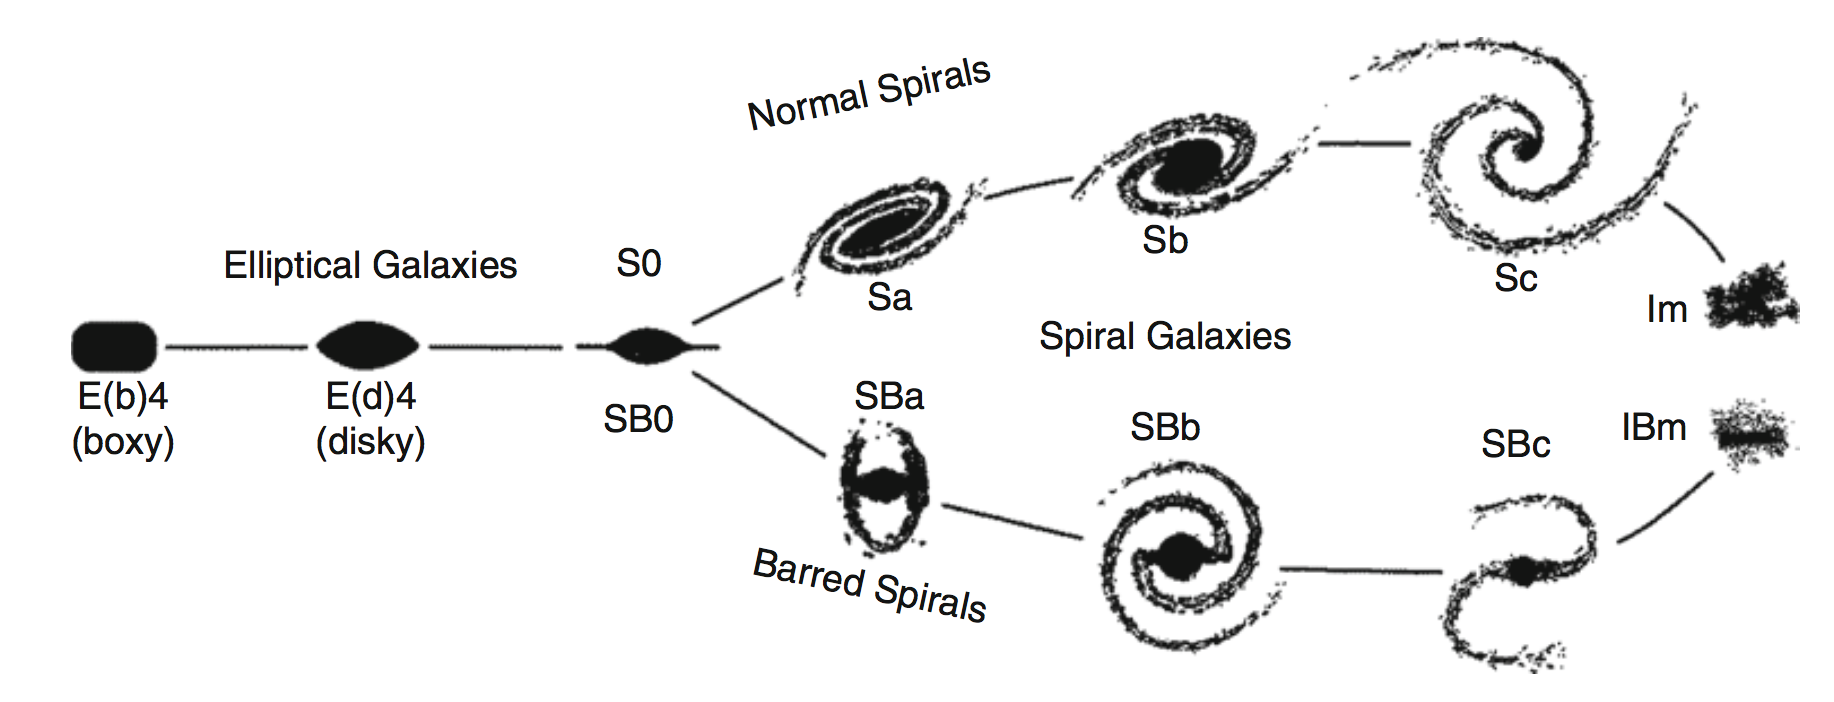
\includegraphics[width=16cm]{figures/HubbleSequence.png}
    \caption{\footnotesize{Hubble’s `tuning fork' for galaxy classification. Adapted from: J. Kormendy \& R. Bender 1996, A Proposed Revision of the Hubble Sequence for Elliptical Galaxies, ApJ 464, L119, Fig. 1. Image taken from Schneider (2006).}}
    \label{fig:hubblesequence}
\end{figure}

\begin{itemize}
    \item Most luminous galaxies in the local Universe fit onto the Hubble sequence; they are either ellipticals, spirals, or belong to the class of S0 galaxies, which shares some properties with the two other classes.
    \item Spiral galaxies consist of a disk with spiral arm structure and a central bulge. They are divided into two subclasses: normal spirals (S's) and barred spirals (SB's).
    \item Elliptical galaxies (E's) are galaxies that have nearly elliptical isophotes without any clearly defined structure.
    \item S0 galaxies are a transition between ellipticals and spirals which are also called lenticulars as they are lentil-shaped galaxies. They contain a bulge and a large enveloping region of relatively unstructured brightness which often appears like a disk without spiral arms.
    \item Irregular galaxies (Irr's) are galaxies with only weak (Irr I) or no (Irr II) regular structure.
    \item Spirals contain a sizable fraction of gas, whereas the gas-to-stellar mass ratio in ellipticals is much smaller. As a consequence, spirals have ongoing star formation, ellipticals not, or only very little. As a further consequence, the light of elliptical galaxies is substantially redder than that of spirals.
    \item The stars in spirals have a very ordered motion, moving around the galactic center on nearly circular orbits in a common orbital plane, having a velocity dispersion that is much smaller than the orbital velocity; the stars in the disk are called `dynamically cold'. In contrast, the motion of stars in ellipticals is largely random, with fairly little coherent velocity; they are `dynamically hot'.
\end{itemize}

\subsubsection{Additional context}

Historically, optical photometry was the method used to observe galaxies. Thus, the morphological classification defined by Hubble is still the best-known today. Besides morphological criteria, color indices, spectroscopic parameters (based on emission or absorption lines), the broad-band spectral distribution (galaxies with/without radio- and/or X-ray emission, or emission in the infrared), as well as other features may also be used.

{\noindent}Figure \ref{fig:hubblesequence} shows the classification scheme defined by Hubble. According to this, three main types of galaxies exist:

\begin{itemize}
    \item \textbf{Elliptical galaxies} (E's) are galaxies that have nearly elliptical isophotes without any clearly defined structure. They are subdivided according to their ellipticity $\epsilon\equiv1-b/a$, where $a$ and $b$ denote the semi-major and the semi-minor axes, respectively. Ellipticals are found over a relatively broad range in ellipticity, $0\leq\epsilon\leq0.7$. The notation E$n$ is commonly used to classify the ellipticals with respect to $\epsilon$, with $n=10\epsilon$; i.e., an E4 galaxy has an axis ratio of $b/a=0.6$, and E0's have circular isophotes.
    \item \textbf{Spiral galaxies} consist of a disk with spiral arm structure and a central bulge. They are divided into two subclasses: normal spirals (S's) and barred spirals (SB's). In each of these subclasses, a sequence is defined that is ordered according to the brightness ratio of bulge and disk, and that is denoted by a, ab, b, bc, c, cd, d. Objects along this sequence are often referred to as being either an early- type or a late-type; hence, an Sa galaxy is an early-type spiral, and an SBc galaxy is a late-type barred spiral. It's stressed explicitly that this nomenclature is not a statement of the evolutionary stage of the objects but is merely a nomenclature of purely historical origin.
    \item \textbf{Irregular galaxies} (Irr's) are galaxies with only weak (Irr I) or no (Irr II) regular structure. The classification of Irr's is often refined. In particular, the sequence of spirals is extended to the classes Sdm, Sm, Im, and Ir (m stands for Magellanic; the Large Magellanic Cloud is of type SBm).
    \item \textbf{S0 galaxies} are a transition between ellipticals and spirals which are also called lenticulars as they are lentil-shaped galaxies. They contain a bulge and a large enveloping region of relatively unstructured brightness which often appears like a disk without spiral arms. Ellipticals and S0 galaxies are referred to as early-type galaxies, spirals as late-type galaxies. As before, these names are only historical and are not meant to describe an evolutionary track!
\end{itemize}

{\noindent}The morphological classification is at least partially affected by projection effects. If, for instance, the spatial shape of an elliptical galaxy is a triaxial ellipsoid, then the observed ellipticity will depend on its orientation with respect to the line-of-sight. Also, it will be difficult to identify a bar in a spiral that is observed from its side (`edge-on').

{\noindent}Besides the aforementioned main types of galaxy morphologies, others exist which do not fit into the Hubble scheme. Many of these are presumably caused by interaction between galaxies. Furthermore, we observe galaxies with radiation characteristics that differ significantly from the spectral behavior of `normal' galaxies.

{\noindent}In summary:

\begin{itemize}
    \item Most luminous galaxies in the local Universe fit onto the Hubble sequence; they are either ellipticals, spirals, or belong to the class of S0 galaxies, which shares some properties with the two other classes.
    \item Ellipticals and spirals differ not only in their morphology, but in several other respects, for example: (1) Spirals contain a sizable fraction of gas, whereas the gas-to- stellar mass ratio in ellipticals is much smaller. As a consequence, (2) spirals have ongoing star formation, ellipticals not, or only very little. As a further consequence, (3) the light of elliptical galaxies is substantially redder than that of spirals. Obviously, the morphology of galaxies and the properties of their stellar populations are strongly correlated.
    \item The stars in spirals have a very ordered motion, moving around the galactic center on nearly circular orbits in a common orbital plane, having a velocity dispersion that is much smaller than the orbital velocity; the stars in the disk are called `dynamically cold'. In contrast, the motion of stars in ellipticals is largely random, with fairly little coherent velocity; they are dynamically hot.
    \item Some elliptical galaxies show clear signs of complex structure, which are interpreted as indications of past interaction with other galaxies. In contrast, the disks of spirals are very thin, which means that they have been largely unperturbed for a long while in the past.
    \item The rotation curves of spiral galaxies are almost flat for large radii, in contrast to what would be expected from the visible mass distribution that declines exponentially outwards. This implies that there is more matter than seen in stars and gas -- the galaxies are embedded in a halo of dark matter. Whereas for elliptical galaxies the radial density distribution is more difficult to probe, the presence of dark matter has been verified also for ellipticals.
    \item Both spirals and ellipticals follow scaling relations which connect their luminous properties (luminosity or surface brightness) with their dynamical properties (rotational velocity or velocity dispersion). Hence, the formation and evolution of galaxies and their stellar populations must proceed in a way as to place them onto these scaling relations.
\end{itemize}

{\noindent}The light from `normal' galaxies is emitted mainly by stars. Therefore, the spectral distribution of the radiation from such galaxies is in principle a superposition of the spectra of their stellar population. The spectrum of stars is, to a first approximation, described by a Planck function that depends only on the star's surface temperature. A typical stellar population covers a temperature range from a few thousand Kelvin up to a few tens of thousand Kelvin. Since the Planck function has a well-localized maximum and from there steeply declines to both sides, most of the energy of such `normal' galaxies is emitted in a relatively narrow frequency interval that is located in the optical and NIR sections of the spectrum.

\begin{figure}[t]
    \centering
    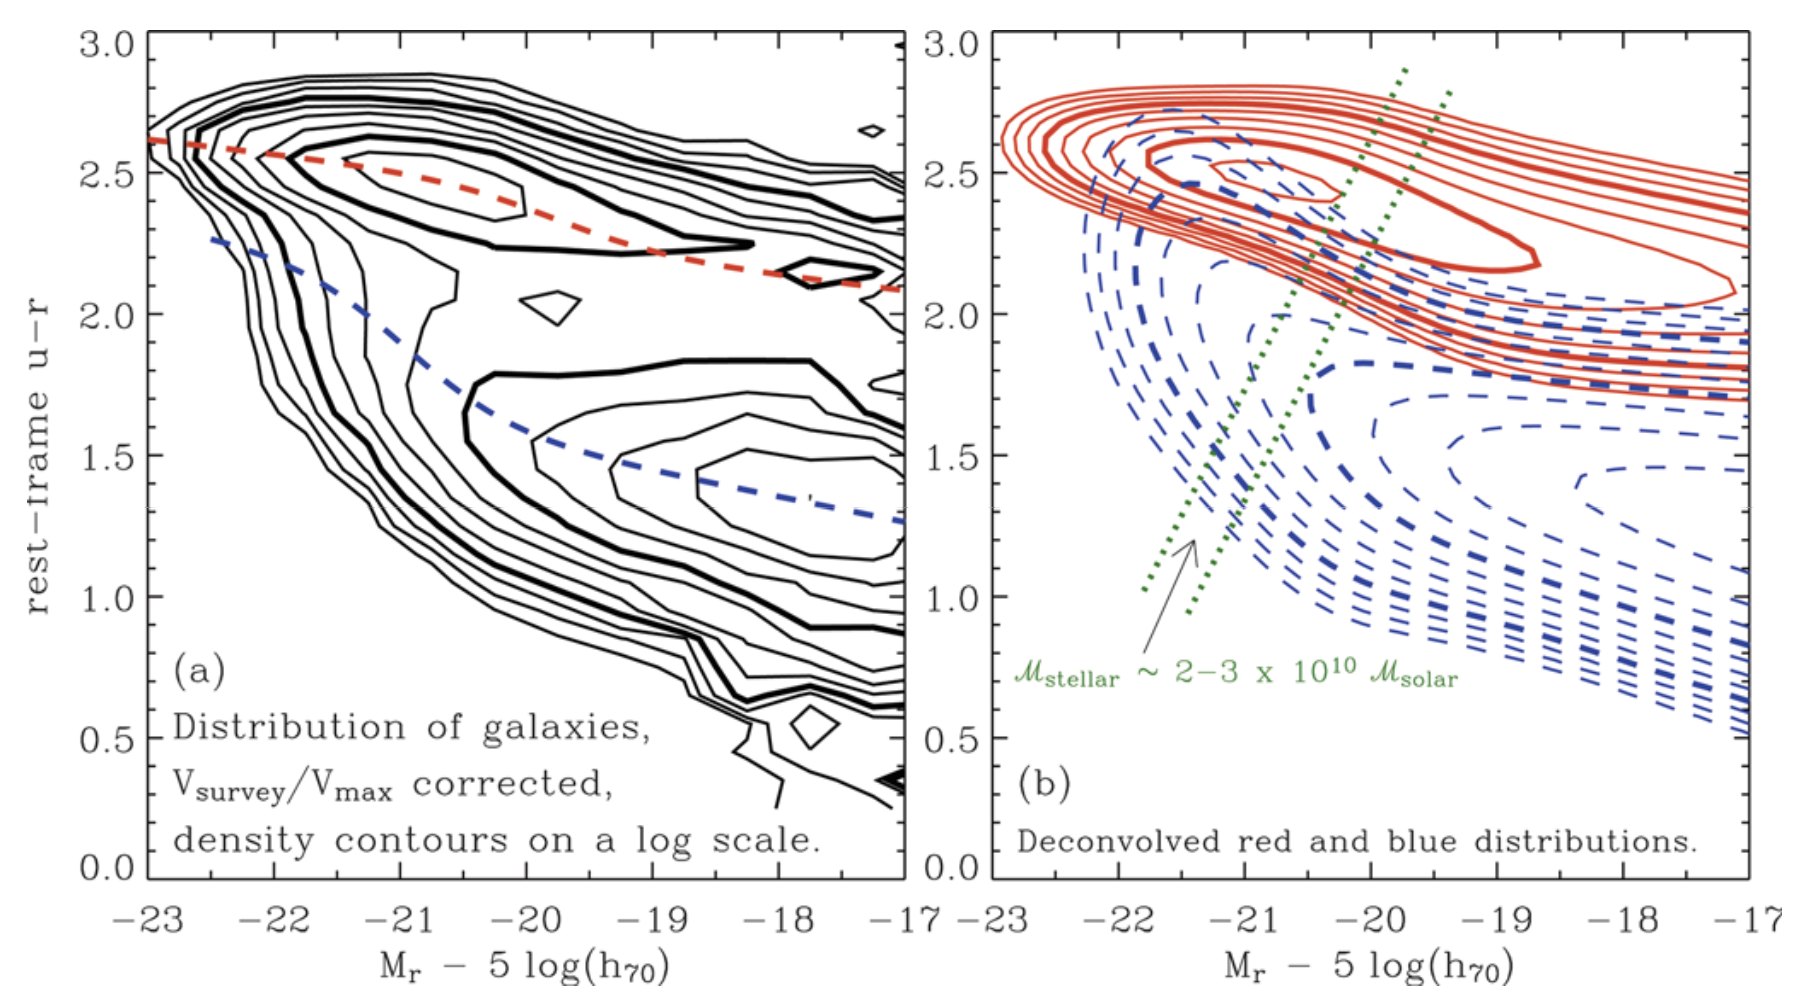
\includegraphics[width=16cm]{figures/SDSSCMD.png}
    \caption{\footnotesize{The density of galaxies in color-magnitude space. The color of $\sim70000$ galaxies with redshifts $0.01\leq z\leq0.08$ from the SDSS is measured by the rest-frame $u-r$, i.e., after a (small) correction for their redshift was applied. The density contours, which were corrected for selection effects, are logarithmically spaced, with a factor of $\sqrt{2}$ between consecutive contours. (a) The measured distribution is shown. Obviously, two peaks of the galaxy density are clearly visible, one at a red color of $u-r\sim2.5$ and an absolute magnitude of $M_r\sim21$,the other at a bluer colour of $u-r\sim1.3$ and significantly fainter magnitudes. (b) Corresponds to the modeled galaxy density. Reused with permission from I.K. Baldry, M.L. Balogh, R. Bower, K. Glazebrook \& R.C. Nichols 2004, Color bimodality: Implications for galaxy evolution, in: THE NEW COSMOLOGY: Conference on Strings and Cosmology, R. Allen (ed.), Conference Proceeding 743, p. 106, Fig. 1 (2004). Figure taken from Schneider (2006).}}
    \label{fig:sdsscmd}
\end{figure}

{\noindent}The classification of galaxies by morphology, given by the Hubble classification scheme (Figure \ref{fig:hubblesequence}), has the disadvantage that morphologies of galaxies are not easy to quantify. Traditionally, this was done by visual inspection but of course this method bears some subjectivity of the researcher doing it and requires a lot of experience. Furthermore, this visual inspection is time consuming and cannot be performed on large samples of galaxies. Various techniques and related software were developed to perform such a classification automatically, in many cases with significant success, including the reproducibility of galaxy classification between different methods. Nevertheless, quite a number of problems remain, such as the inclination dependence of the morphological appearance of a galaxy.

{\noindent}Even automatic classifications cannot be applied to galaxies for which the angular resolution of the imaging is not much better than the angular size of galaxies, that is, for distant objects. An alternative to morphological classification is provided by the colours of galaxies, which can be obtained from broad-band multi-color imaging. Colors are much easier to measure than morphology, in particular for very small galaxies. In addition, the physical properties of galaxies may be better characterized by their colors than by their morphology -- the colours yield information about the stellar population, whereas the morphology is determined by the dynamics of the galaxy.

{\noindent}Using photometric measurements and spectroscopy from the SDSS, the colours and absolute magnitudes of low-redshift galaxies have been studied; their density distribution in a color-magnitude diagram is plotted in the left-hand side of Figure \ref{fig:sdsscmd}. We see immediately that there are two density peaks of the galaxy distribution in this diagram: one at high luminosities and red color, the other at significantly fainter absolute magnitudes and much bluer color. It appears that the galaxies are distributed at and around these two density peaks, hence galaxies tend to be either luminous and red, or less luminous and blue. We can also easily see from this diagram that the distribution of red and blue galaxies with respect to their luminosity is different, the former one being more shifted towards larger luminosity.

{\noindent}We can next consider the color distribution of galaxies at a fixed absolute magnitude $M_r$. This is obtained by plotting the galaxy number density along vertical cuts through the left-hand side of Figure \ref{fig:sdsscmd}. When this is done for different $M_r$, it turns out that the colour distribution of galaxies is bimodal: over a broad range in absolute magnitude, the color distribution has two peaks, one at red, the other at blue $u-r$. Again, this fact can be seen directly from Figure \ref{fig:sdsscmd}. For each value of $M_r$, the colour distribution of galaxies can be very well fitted by the sum of two Gaussian functions. The central colors of the two Gaussians are shown by the two dashed curves in the left panel of Figure \ref{fig:sdsscmd}. They become redder the more luminous the galaxies are. This luminosity-dependent reddening is considerably more pronounced for the blue population than for the red galaxies.

{\noindent}To see how good this fit indeed is, the right-hand side of Figure \ref{fig:sdsscmd} shows the galaxy density as obtained from the two-Gaussian fits, with solid contours corresponding to the red galaxies and dashed contours to the blue ones. We thus conclude that the local galaxy population can be described as a bimodal distribution in $u-r$ color, where the characteristic color depends slightly on absolute magnitude. The galaxy distribution at bright absolute magnitudes is dominated by red galaxies, whereas for less luminous galaxies the blue population dominates.

{\noindent}The mass-to-light ratio of a red stellar population is larger than that of a blue population, since the former no longer contains massive luminous stars. The difference in the peak absolute magnitude between the red and blue galaxies therefore corresponds to an even larger difference in the stellar mass of these two populations. Red galaxies in the local Universe have on average a much higher stellar mass than blue galaxies. This fact is illustrated by the two dotted lines in the right-hand panel of Figure \ref{fig:sdsscmd} which correspond to lines of constant stellar mass of $\sim2-3\times10^{10}\,{\rm M}$. This seems to indicate a very characteristic mass scale for the galaxy distribution: most galaxies with a stellar mass larger than this characteristic mass scale are red, whereas most of those with a lower stellar mass are blue.

\begin{table}[t]
    \centering
    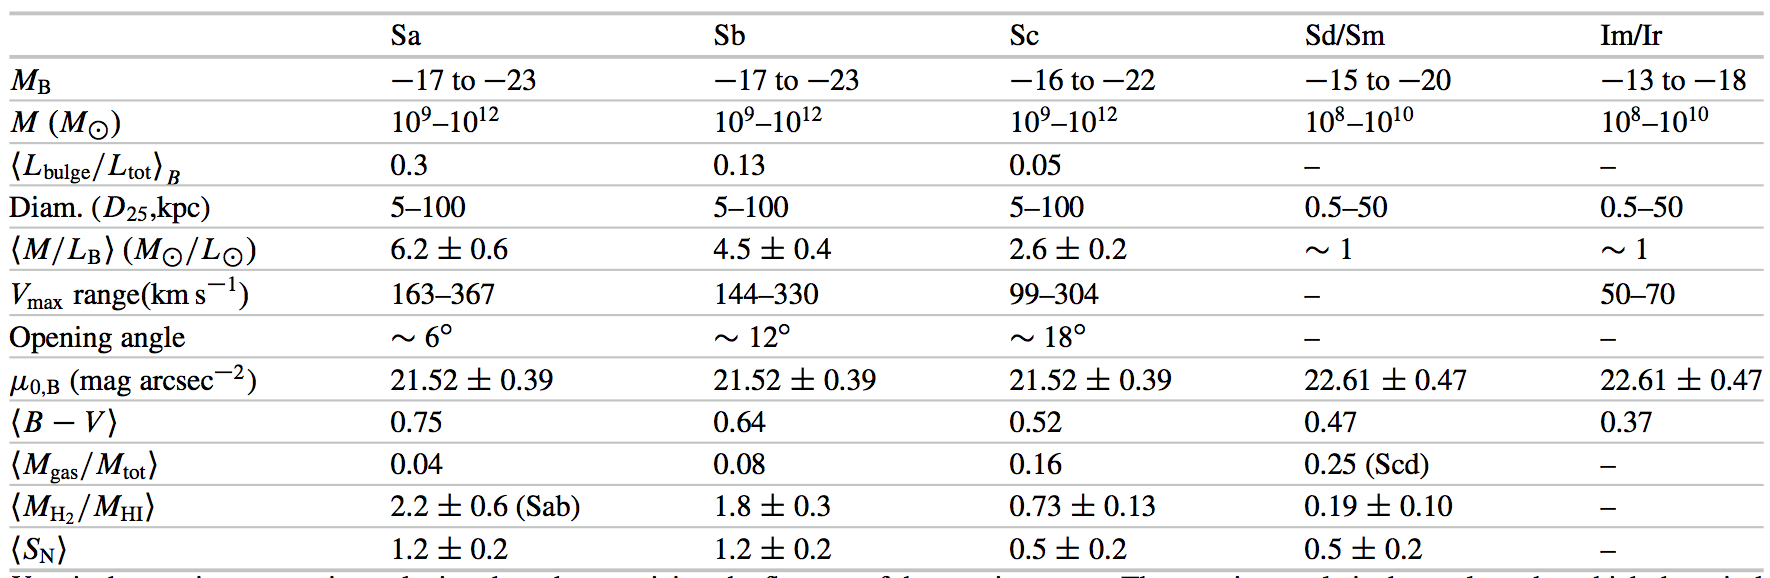
\includegraphics[width=16cm]{figures/LateGalaxies.png}
    \caption{\footnotesize{Characteristic values for late-type (i.e., spiral) galaxies. $V_\mathrm{max}$ is the maximum rotation velocity, thus characterizing the flat part of the rotation curve. The opening angle is the angle under which the spiral arms branch off, i.e., the angle between the tangent to the spiral arms and the circle around the center of the galaxy running through this tangential point. $S_N$ is the specific abundance of globular clusters. The values in this table are taken from the book by Carroll \& Ostlie. Table taken from Schneider (2006).}}
    \label{table:lategalaxies}
\end{table}

{\noindent}Looking at the sequence of early-type spirals (i.e., Sa's or SBa's) to late-type spirals, we find a number of differences that can be used for classification:

\begin{itemize}
    \item A decreasing luminosity ratio of bulge and disk, with $L_\mathrm{bulge}/L_\mathrm{disk}\sim0.3$ for Sa’s and $\sim0.05$ for Sc’s
    \item An increasing opening angle of the spiral arms, from   $6^\circ$ for Sa's to $18^\circ$ for Sc's.
    \item An increasing brightness structure along the spiral arms: Sa's have a `smooth' distribution of stars along the spiral arms, whereas the light distribution in the spiral arms of Sc's is resolved into bright knots of stars and HII regions.
\end{itemize}

{\noindent}Bars are common in spiral galaxies, with $\sim70\%$ of all disk galaxies containing a large-scale stellar bar. Such a bar perturbs the axial symmetry of the gravitational potential in a galaxy, which may have a number of consequences. One of them is that this perturbation can lead to a redistribution of angular momentum of the stars, gas, and dark matter. In addition, by perturbing the orbits, gas can be driven towards the center of the galaxy which may have important consequences for triggering nuclear activity and enhanced star formation.

{\noindent}The light profile of the bulge of spirals is described by a \textbf{de Vaucouleurs profile} to a first approximation, while the disk follows an exponential brightness profile, as is the case for our MW. Expressing these distributions of the surface brightness in $\mu\propto-2.5\log(I)$, measured in ${\rm mag\,arcsec^{-2}}$, we obtain

\begin{align*}
    \mu_\mathrm{bulge} = \mu_e + 8.3268\left[\left(\frac{R}{R_e}\right)^{1/4}-1\right] ~ [{\rm mag\,arcsec^{-2}}]
\end{align*}

{\noindent}and

\begin{align*}
    \mu_\mathrm{disk} = \mu_0 + 1.09\left(\frac{R}{h_R}\right) ~ [{\rm mag\,arcsec^{-2}}].
\end{align*}

{\noindent}Here, $\mu_e$ is the surface brightness at the effective radius $R_e$ which is defined such that half of the bulge luminosity is emitted within $R_e$. The central surface brightness and the scale-length of the disk are denoted by $\mu_0$ and $h_R$, respectively. It has to be noted that $\mu_0$ is not directly measurable since $\mu_0$ is not the central surface brightness of the galaxy, only that of its disk component. To determine $\mu_0$, the exponential law is extrapolated from large $R$ inwards to $R=0$, or more precisely, by fitting the sum of an exponential and a bulge component to the total light profile of the galaxy.

{\noindent}The brightness profile of spiral disks perpendicular to the disk can be studied exclusively in edge-on spirals. From them, one finds that it is in general well described by an exponential law. The scale-height $h_z$ of the disk is almost independent of the galacto-centric radius $R$, and between galaxies scales roughly linearly with the rotational velocity of the disk. The typical value for the ratio of scale-height to scale-length is $h_z/h_R=0.07$ -- indeed, the disks of spiral galaxies are thin. The flattest galaxies are those of late Hubble type.

{\noindent}While the brightness profile of bulges follows approximately that of a de Vaucouleurs profile, some spiral galaxies bulges were found which behave differently than these `classical' bulges; one calls them \textbf{pseudobulges}. In contrast to classical bulges, they follow more an exponential profile, are typically flatter, and have significant rotational support. Furthermore, whereas classical bulges lie on the same sequence in the effective radius vs. absolute magnitude diagram as the ellipticals, pseudobulges do not. They have lower luminosity for a given size.

{\noindent}In many cases it is very difficult to distinguish between both types of bulges photometrically. However, spectroscopy aids a lot in this distinction. In fact, some bulges of spirals have two components, i.e., both a classical bulge and a pseudobulge.

{\noindent}The differences in the two types of bulges suggest that they should have a different origin. Classical bulges behave like a small elliptical galaxy. It is believed that ellipticals form through merging events of galaxies which `heats up' the stellar velocity distribution (i.e., turns ordered velocity fields of disk galaxies into random orbits which are characteristic for ellipticals). Therefore, in the current model of galaxy evolution, classical bulges are also formed as a result of merger events. In contrast, the ordered rotation of pseudobulges suggests that they have evolved from the disk population. For example, symmetry perturbations of the gravitational field caused by a bar can generate random velocity components of stars perpendicular to the plane of the disk, and thus thicken the disk population in the inner part of a galaxy.

{\noindent}Whereas pseudobulges may provide important insights into the evolution of galaxies, they are a sub-dominant component in the population of galaxies. It is estimated that classical bulges together contain about ten times more stars than pseudobulges. Therefore, whenever the term `bulge' is used, it's often implicitly meant to refer to the classical bulges.

{\noindent}Some late-type spiral galaxies seem to have no bulge component. Some of them show instead a nuclear stellar cluster at their center. These nuclear star clusters appear at first sight to be similar to globular clusters. However, their stellar population is quite different from that of the old globular clusters in our Galaxy, as their light is dominated by a relatively young stellar population, although their stellar mass is totally dominated by an old population. In some respect, these nuclear star clusters share properties with the peculiar Galactic globular $\omega$ Centauri, which also shows a broad range of stellar ages and an inhomogeneous chemical abundance. Therefore, it has been hypothesized that $\omega$ Centaurus is the remnant of a merger of a lower mass galaxy with the MW.

{\noindent}The general term `elliptical galaxies' (or ellipticals, for short) covers a broad class of galaxies which differ in their luminosities and sizes. A rough subdivision is as follows:

\begin{itemize}
    \item \textbf{Normal ellipticals}: This class includes giant ellipticals (gE's), those of intermediate luminosity (E's), and compact ellipticals (cE's), covering a range in absolute magnitudes from $M_B\sim23$ to $M_B\sim15$.
    \item \textbf{Dwarf ellipticals (dE's)}: These differ from the cE's in that they have a significantly smaller surface brightness and a lower metallicity.
    \item \textbf{cD galaxies}: These are extremely luminous (up to $M_B\sim25$) and large (up to $R\sim1{\rm Mpc}$) galaxies that are only found near the centers of dense clusters of galaxies. Their surface brightness is very high close to the center, they have an extended diffuse envelope, and they have a very high $M/L$ ratio. It is not clear whether the extended envelope actually `belongs' to the galaxy or is part of the galaxy cluster in which the cD is embedded, since such clusters are now known to have a population of stars located outside of the cluster galaxies.
    \item \textbf{Blue compact dwarf galaxies}: These `blue compact dwarfs' (BCD’s) are clearly bluer (with $(B-V)$ between $0.0$ and $0.3$) than the other ellipticals, and contain an appreciable amount of gas in comparison.
    \item \textbf{Dwarf spheroidals (dSph's)}: These exhibit a very low luminosity and surface brightness. They have been observed down to $M_B\sim8$. Due to these properties, they have thus far only been observed in the Local Group.
\end{itemize}

\begin{table}[t]
    \centering
    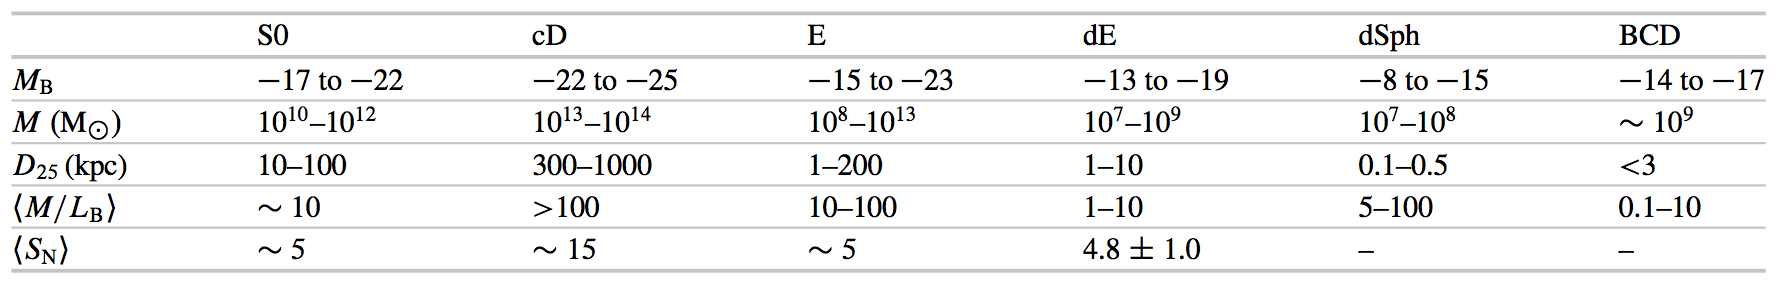
\includegraphics[width=16cm]{figures/EarlyGalaxies.png}
    \caption{\footnotesize{Characteristic values for early-type galaxies. $D_{25}$ denotes the diameter at which the surface brightness has decreased to $25\,{\rm B-mag\,arcsec^{-2}}$ , $S_N$ is the `specific frequency', a measure for the number of globular clusters in relation to the visual luminosity, and $M/L$ is the mass-to-light ratio in Solar units. The values of this table are taken from the book by Carroll \& Ostlie. Table taken from Schneider (2006).}}
    \label{table:earlygalaxies}
\end{table}

{\noindent}Analyzing the morphology of elliptical galaxies raises a simple question: Why are ellipticals not round? A simple explanation would be rotational flattening, i.e., as in a rotating self-gravitating gas ball, the stellar distribution bulges outwards at the equator due to centrifugal forces, as is also the case for the Earth. If this explanation was correct, the rotational velocity $v_\mathrm{rot}$, which is measurable in the relative Doppler shift of absorption lines, would have to be of about the same magnitude as the velocity dispersion of the stars $\sigma_v$ that is measurable through the Doppler broadening of lines. More precisely, by means of stellar dynamics one can show that for the rotational flattening of an axially symmetric, oblate galaxy, the relation

\begin{align*}
    \left(\frac{v_\mathrm{rot}}{\sigma_v}\right)_\mathrm{iso} = \sqrt{\frac{\epsilon}{1-\epsilon}} ~ [{\rm dimensionless}]
\end{align*}

{\noindent}has to be satisfied, where `iso' indicates the assumption of an isotropic velocity distribution of the stars. However, for very luminous ellipticals one finds that, in general, $v_\mathrm{rot}\ll \sigma_v$, so that rotation cannot be the major cause of their ellipticity. In addition, many ellipticals are presumably triaxial, so that no unambiguous rotation axis is defined. Thus, luminous ellipticals are in general not rotationally flattened. For less luminous ellipticals and for the bulges of disk galaxies, however, rotational flattening can play an important role. The question remains of how to explain a stable elliptical distribution of stars without bulk rotation.

{\noindent}The brightness profile of an elliptical galaxy is defined by the distribution of its stellar orbits. Let us assume that the gravitational potential is given. The stars are then placed into this potential, with the initial positions and velocities following a specified distribution. If this distribution is not isotropic in velocity space, the resulting light distribution will in general not be spherical. For instance, one could imagine that the orbital planes of the stars have a preferred direction, but that an equal number of stars exists with positive and negative angular momentum $L_z$, so that the total stellar distribution has no net angular momentum and therefore does not rotate. Each star moves along its orbit in the gravitational potential, where the orbits are in general not closed. If an initial distribution of stellar orbits is chosen such that the statistical properties of the distribution of the orbits are invariant in time, then one will obtain a stationary system. If, in addition, the distribution is chosen such that the respective mass distribution of the stars will generate exactly the originally chosen gravitational potential, one arrives at a self-gravitating equilibrium system. In general, it is a difficult mathematical problem to construct such self-gravitating equilibrium systems. Furthermore, elliptical galaxies also contain a dark matter component, whose gravitational potential adds to that of the stars.

{\noindent}The question now arises whether such an equilibrium system can also be stable in time. One might expect that close encounters of pairs of stars would cause a noticeable disturbance in the distribution of orbits. These pair-wise collisions could then lead to a `thermalization' of the stellar orbits. To examine this question we need to estimate the time-scale for such collisions and the changes in direction they cause.

{\noindent}For this purpose, we consider the relaxation time-scale by pair collisions in a system of $N$ stars of mass $m$, total mass $M=Nm$, extent $R$, and a mean stellar density of $n=3N/(4\pi R^3)$. We define the relaxation time $t_\mathrm{relax}$ as the characteristic time in which a star changes its velocity direction by $\sim90^\circ$ due to pair collisions with other stars. By simple calculation (see below), we find that

\begin{align*}
    t_\mathrm{relax} \approx \frac{R}{6v} \frac{N}{\ln(N/2)} ~ [{\rm yr}]
\end{align*}

{\noindent}or

\begin{align*}
    t_\mathrm{relax} = \frac{t_\mathrm{cross}}{6} \frac{N}{\ln(N/2)} ~ [{\rm yr}],
\end{align*}

{\noindent}where $t_\mathrm{cross}=R/v$ is the crossing time-scale, i.e. the time it takes a star to cross the stellar system. If we now consider a typical galaxy, with $t_\mathrm{cross}\sim10^8\,{\rm yr}$, $N\sim10^{12}$ (thus $ln(N/2)\sim30$), then we find that the relaxation time is much longer than the age of the Universe. This means that pair collisions do not play any role in the evolution of stellar orbits. The dynamics of the orbits are determined solely by the large-scale gravitational field of the galaxy. There is a process called violent relaxation which most likely plays a central role in the formation of galaxies and which is probably also responsible for the stellar orbits establishing an equilibrium configuration.

{\noindent}We thus conclude that the stars behave like a collisionless gas: elliptical galaxies are stabilized by (dynamical) pressure, and they are elliptical because the stellar distribution is anisotropic in velocity space. This corresponds to an anisotropic pressure -- where we recall that the pressure of a gas is nothing but the momentum transport of gas particles due to their thermal motion.


\subsubsection{Follow-up Questions}

\begin{itemize}
    \item What physical trends does the Hubble sequence show that were not explicitly encoded in it? (i.e., spiral arm tightness and bulge size are properties that Hubble based the sequence off of.)
    \item Are there any other physical properties that the Hubble sequence ended up telling us about (i.e., by `accident')?
    \item Do most observable galaxies fall somewhere on the Hubble sequence?
    \item Describe how galaxies form and evolve.
\end{itemize}


% --------------------------------------------------------------
%               2. 
% --------------------------------------------------------------

\newpage
\subsection{Question 2}

What is the total mass (in both dark matter and in stars) of the Milky Way galaxy? How does this compare to M31 and to the LMC? How is this mass determined?

\subsubsection{Short answer}

The MWG has a total mass of about $10^{12}\,{\rm M_\odot}$. This is about the same as M31 (Andromeda), and larger than the LMC which is roughly $10^{10}\,{\rm M_\odot}$. Assuming virial equlibrium, the mass can be determined from the flat part of the rotation curve via

\begin{align*}
    V_0 = \sqrt{\frac{GM(<R)}{R_0}} ~ [{\rm m\,s^{-1}}].
\end{align*}

{\noindent}If spiral galaxies are being observed, the Tully-Fisher relation $L\propto v_\mathrm{max}^4$ can be used to determine the maximum orbital velocity in replacement of the rotation curve. Similarly, if elliptical galaxies are being observed, the Faber-Jackson relation $L\propto\sigma_v^4$ can be used instead.

\subsubsection{Additional context}

The components of the Milky Way Galaxy (MWG) have total masses as follows: a disk mass of $4.5\times10^{10}\,{\rm M_\odot}$, bulge mass of $4.5\times10^9\,{\rm M_\odot}$, dark halo mass of $2\times10^{12}\,{\rm M_\odot}$, and BH mass of $4\times10^6\,{\rm M_\odot}$.

{\noindent}The Galactic disk rotates, with rotational velocity $V(R)$ depending on the distance $R$ from the center. We can estimate the mass of the Galaxy from the distribution of the stellar light and the mean mass-to-light ratio of the stellar population, since gas and dust represent less than $\sim10$\% of the mass of the stars. From this mass estimate we can predict the rotational velocity as a function of radius simply from Newtonian mechanics. However, the observed rotational velocity of the Sun around the Galactic center is significantly higher than would be expected from the observed mass distribution. If $M(<R_0)$ is the mass inside a sphere around the Galactic center with radius $R_0=8\,{\rm kpc}$, then the rotational velocity from Newtonian mechanics is

\begin{align*}
    V_0 = \sqrt{\frac{GM(<R)}{R_0}} ~ [{\rm m\,s^{-1}}].
\end{align*}

{\noindent}From the visible matter in stars we would expect a rotational velocity of $160\,{\rm km\,s}$, but we observe $V_0=220\,{\rm km\,s}$ (see Figure \ref{fig:rotationcurve}). This discrepancy, and the shape of the rotation curve $V(R)$ for larger distances $R$ from the Galactic center, indicates that our Galaxy contains significantly more mass than is visible in the form of stars. This additional mass is called dark matter. Its physical nature is still unknown. The main candidates are weakly interacting elementary particles like those postulated by some elementary particle theories, but they have yet not been detected in the laboratory. Macroscopic objects (i.e., celestial bodies) are also in principle viable candidates if they emit very little light.

\begin{figure}[h]
    \floatbox[{\capbeside\thisfloatsetup{capbesideposition={right,top},capbesidewidth=4cm}}]{figure}[\FBwidth]
    {\caption{\footnotesize{The upper curve is the observed rotation curve $V(R)$ of our Galaxy, i.e., the rotational velocity of stars and gas around the Galactic center as a function of their galacto-centric distance. The lower curve is the rotation curve that we would predict based solely on the observed stellar mass of the Galaxy. The difference between these two curves is ascribed to the presence of dark matter, in which the Milky Way disk is embedded. This image is adapted from Nick Strobel's webpage at \href{www.astronomynotes.com}{www.astronomynotes.com}. Image taken from Schneider (2006).}}
    \label{fig:rotationcurve}}
    {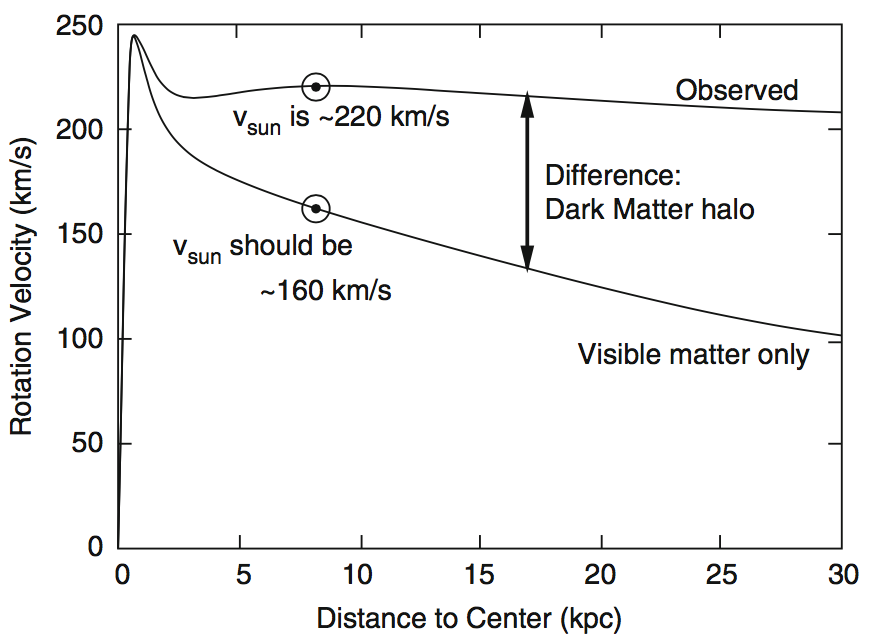
\includegraphics[width=10cm]{figures/RotationCurve.png}}
\end{figure}

\newpage
\subsubsection{Follow-up Questions}

\begin{itemize}
    \item If rotation curve/lensing measurements were instead due to modified gravity, how could we tell?
    \item What are $\Omega_m$ and $\Omega_b$ estimated to be? Why does the ratio of the two differ from the star/total mass ratio you have here? Where is all the extra baryonic mass?
    \item When you say we estimate stellar mass by ``counting stars'', what does that mean?
\end{itemize}

% --------------------------------------------------------------
%               3. 
% --------------------------------------------------------------

\newpage
\subsection{Question 3}

Describe as many steps of the distance ladder and the involved techniques as you can. What are the rough distances to the Magellanic Clouds, Andromeda, and the Virgo Cluster?

\subsubsection{Short answer}

The rough distances to the Magellanic Clouds, Andromeda, and the Virgo Cluster are as follows:

\begin{align*}
    d_\mathrm{LMC} \approx 50 ~ [{\rm kpc}] \\
    d_\mathrm{SMC} \approx 60 ~ [{\rm kpc}] \\
    d_\mathrm{M31} \approx 700 ~ [{\rm kpc}] \\
    d_\mathrm{Virgo} \approx 10 ~ [{\rm Mpc}].
\end{align*}

\subsubsection{Additional context}

{\noindent}\textbf{Trigonometric parallax ($<30\,{\rm pc}$)}: The most important method of distance determination is the trigonometric parallax, not only from a historical point-of-view. This method is based on a purely geometric effect and is therefore independent of any physical assumptions. Due to the motion of the Earth around the Sun the positions of nearby stars on the sphere change relative to those of very distant sources (e.g., extragalactic objects such as quasars). The latter therefore define a fixed reference frame on the sphere. In the course of a year the apparent position of a nearby star follows an ellipse on the sphere, the semi-major axis of which is called the parallax. The axis ratio of this ellipse depends on the direction of the star relative to the ecliptic (the plane that is defined by the orbits of the Earth and the other planets). The parallax depends on the radius $r$ of the Earth’s orbit, hence on the Earth-Sun distance which is, by definition, one astronomical unit (AU). Furthermore, the parallax depends on the distance $d$ of the star,

\begin{align*}
    \frac{r}{d} = \tan(p) \approx p ~ [{\rm rad}].
\end{align*}

{\noindent}where we used $p\ll1$ in the last step, and $p$ is measured in radians as usual. The trigonometric parallax is also used to define the common unit of distance in astronomy: one parsec (pc) is the distance of a hypothetical source for which the parallax is exactly $p=1''$. With the conversion of arcseconds to radians ($1''\approx4.848\times10^{-6}\,{\rm rad}$) one gets $p/1''=206265p$, which for a parsec yields

\begin{align*}
    1\,{\rm pc} = 206265\,{\rm AU} = 3.086\times10^{16}\,{\rm m}.
\end{align*}

{\noindent}The distance corresponding to a measured parallax is then
calculated as

\begin{align*}
    d = \left(\frac{p}{1''}\right)^{-1}\,{[\rm pc]}.
\end{align*}

{\noindent}o determine the parallax p, precise measurements of the position of an object at different times are needed, spread over a year, allowing us to measure the ellipse drawn on the sphere by the object’s apparent position. For ground-based observations the accuracy of this method is limited by the atmosphere. The seeing causes a blurring of the images of astronomical sources and thus limits the accuracy of position measurements. From the ground this method is therefore limited to parallaxes larger than $\approx0.1''$, implying that the trigonometric parallax yields distances to stars only within $\approx30\,{\rm pc}$.

{\noindent}\textbf{Proper motions}: Stars are moving relative to us or, more precisely, relative to the Sun. To study the kinematics of the Milky Way we need to be able to measure the velocities of stars. The radial component $v_r$ of the velocity is easily obtained from the Doppler shift of spectral lines,

\begin{align*}
    v_r = \left(\frac{\Delta\lambda}{\lambda_0}\right)c ~ [{\rm m\,s^{-1}}]
\end{align*}

{\noindent}where $\lambda_)$ is the rest-frame wavelength of an atomic transition and $\Delta\lambda=\lambda-\lambda_0$ is the Doppler shift of the wavelength due to the radial velocity of the source. The sign of the radial velocity is defined such that $v_r>0$ corresponds to a motion away from us, i.e., to a redshift of spectral lines.

{\noindent}In contrast, the determination of the other two velocity components is much more difficult. The tangential component, $v_t$, of the velocity can be obtained from the proper motion of an object. In addition to the motion caused by the parallax, stars also change their positions on the sphere as a function of time because of the transverse component of their velocity relative to the Sun. The proper motion $\mu$ is thus an angular velocity, e.g., measured in milliarcseconds per year (mas/yr or $''/{\rm year}$). This angular velocity is linked to the tangential velocity component via

\begin{align*}
    v_t = d\mu = 4.74\left(\frac{d}{1\,{\rm pc}}\right) \left(\frac{\mu}{1''\,{\rm year^{-1}}}\right) ~ [{\rm m\,s^{-1}}].
\end{align*}

{\noindent}Therefore, one can calculate the tangential velocity from the proper motion and the distance. If the latter is derived from the trigonometric parallax, these can be combined to yield

\begin{align*}
    v_t = d\mu = 4.74 \left(\frac{\mu}{1\,''\,{\rm year^{-1}}}\right) \left(\frac{p}{1''}\right)^{-1} ~ [{\rm m\,s^{-1}}].
\end{align*}

{\noindent}Of course, the proper motion has two components, corresponding to the absolute value of the angular velocity and its direction on the sphere. Together with $v_r$ this determines the three-dimensional velocity vector. Correcting for the known velocity of the Earth around the Sun, one can then compute the velocity vector v of the star relative to the Sun, called the heliocentric velocity.

{\noindent}\textbf{Moving cluster parallax ($<200\,{\rm pc}$)}: The stars in an (open) star cluster all have a very similar spatial velocity. This implies that their proper motion vectors should be similar. To what accuracy the proper motions are aligned depends on the angular extent of the star cluster on the sphere. Like two railway tracks that run parallel but do not appear parallel to us, the vectors of proper motions in a star cluster also do not appear parallel. They are directed towards a convergence point, as depicted in Figure \ref{fig:clusterparallax}.

\begin{figure}[h]
    \floatbox[{\capbeside\thisfloatsetup{capbesideposition={right,top},capbesidewidth=4cm}}]{figure}[\FBwidth]
    {\caption{\footnotesize{The moving cluster parallax is a projection effect, similar to that known from viewing railway tracks. The directions of velocity vectors pointing away from us seem to converge and intersect at the convergence point. The connecting line from the observer to the convergence point is parallel to the velocity vector of the star cluster. Image taken from Schneider (2006).}}
    \label{fig:clusterparallax}}
    {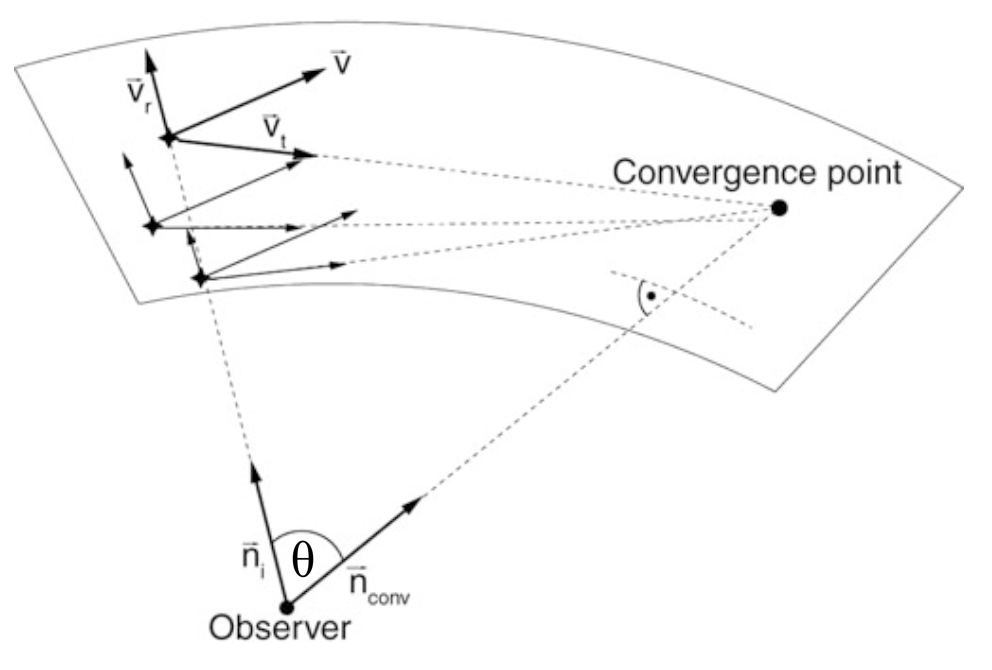
\includegraphics[width=10cm]{figures/ClusterParallax.png}}
\end{figure}

{\noindent}We consider a star cluster and assume that all stars have the same spatial velocity $v$. The position of the i-th star as a function of time is then described by

\begin{align*}
    \mathbf{r}_i(t) = \mathbf{r}_i(t) + \mathbf{v}t ~ [{\rm m}],
\end{align*}

{\noindent}where $\mathbf{r}_i$ is the current position if we identify the origin of time, $t=0$, with `today'. The direction of a star relative to us is described by the unit vector

\begin{align*}
    \mathbf{n}_i(t) \equiv \frac{\mathbf{r}_i}{\lvert\mathbf{r}_i\rvert} ~ [{\rm dimensionless}].
\end{align*}

{\noindent}From this, one infers that for large times, $t\rightarrow\infty$, the direction vectors of the convergence point are identical for all stars in the cluster,

\begin{align*}
    \mathbf{n}_i(t) \rightarrow \frac{\mathbf{v}}{\lvert\mathbf{v}\rvert} \equiv \mathbf{n}_\mathrm{conv} ~ [{\rm dimensionless}].
\end{align*}

{\noindent}Hence for large times all stars will appear at the same point $\mathbf{n}_\mathrm{conv}$: the convergence point. This only depends on the direction of the velocity vector of the star cluster. In other words, the direction vector of the stars is such that they are all moving towards the convergence point. Thus, $\mathbf{n}_\mathrm{conv}$ (and hence $\mathbf{v}/\lvert\mathbf{v}\rvert$) can be measured from the direction of the proper motions of the stars in the cluster. On the other hand, one component of $\mathbf{v}$ can be determined from the (easily measured) radial velocity $\mathbf{v}_r$. With these two observables the three-dimensional velocity vector $\mathbf{v}$ is completely determined, as is easily demonstrated: let $\theta$ be the angle between the line-of-sight $\mathbf{n}$ towards a star in the cluster and $\mathbf{v}$. The angle is directly read off from the direction vector $\mathbf{n}$ and the convergence point, $\cos\theta = \mathbf{n}\cdot\mathbf{v}/\lvert\mathbf{v}\rvert = \mathbf{}_\mathrm{conv}\cdot\mathbf{n}$. With $v\equiv\lvert\mathbf{v}\rvert$ one then obtains

\begin{align*}
    v_r = v\cos\theta ~ [{\rm m\,s^{-1}}], ~~~~~ v_t = v\sin\theta ~ [{\rm m\,s^{-1}}],
\end{align*}

{\noindent}and so

\begin{align*}
    v_t = v_r\tan\theta ~ [{\rm m\,s^{-1}}].
\end{align*}

{\noindent}This means that the tangential velocity $\mathbf{v}_t$ can be measured without determining the distance to the stars in the cluster. On the other hand, we have a relation between the proper motion, the distance, and $\mathbf{v}$. Hence, a distance determination for the star is now possible with

\begin{align*}
    \mu = \frac{v_t}{d} = \frac{v_r\tan\theta}{d} \rightarrow d = \frac{v_r\tan\theta}{\mu} ~ [{\rm pc}].
\end{align*}

{\noindent}This method yields accurate distance estimates of star clusters within $\sim200\,{\rm pc}$. The accuracy depends on the measurability of the proper motions. Furthermore, the cluster should cover a sufficiently large area on the sky for the convergence point to be well defined. For the distance estimate, one can then take the average over a large number of stars in the cluster if one assumes that the spatial extent of the cluster is much smaller than its distance to us.

{\noindent}\textbf{Main sequence fitting}: Most stars in the color-magnitude diagram (CMD) are located along the main sequence. This enables us to compile a calibrated main sequence of those stars whose trigonometric parallaxes are measured, thus with known distances. Utilizing photo- metric methods, it is then possible to derive the distance to a star cluster. 

{\noindent}The stars of a star cluster define their own main sequence; since they are all located at the same distance, their main sequence is already defined in a CMD in which only apparent magnitudes are plotted. This cluster main sequence can then be fitted to a calibrated main sequence by a suitable choice of the distance, i.e., by adjusting the \textbf{distance modulus} $m-M$,

\begin{align*}
    m-M = 5\log(d/{\rm pc}) - 5 ~ [{\rm mag}],
\end{align*}

{\noindent}where $m$ and $M$ denote the apparent and absolute magnitude, respectively.

{\noindent}In reality this method cannot be applied so easily since the position of a star on the main sequence does not only depend on its mass but also on its age and metallicity. Furthermore, only stars of luminosity class V (i.e., dwarf stars) define the main sequence, but without spectroscopic data it is not possible to determine the luminosity class.

{\noindent}\textbf{Extinction and reddening}: Another major problem is extinction. Absorption and scattering of light by dust affect the relation of absolute to apparent magnitude: for a given $M$, the apparent magnitude $m$ becomes larger (fainter) in the case of absorption, making the source appear dimmer. Also, since extinction depends on wavelength, the spectral energy distribution of the source is modified and the observed colour of the star changes. Because extinction by dust is always associated with such a change in colour, one can estimate the absorption -- provided one has sufficient information on the intrinsic colour of a source or of an ensemble of sources.

{\noindent}We consider the \textbf{equation of radiative transfer} for pure absorption or scattering:

\begin{align*}
    \frac{\mathrm{d}I_\nu}{\mathrm{d}s} = -\alpha_\nu I_\nu ~ [\rm erg\,s^{-1}\,cm^{-3}\,ster^{-1}\,Hz^{-1}],
\end{align*}

{\noindent}where $I_\nu$ is the specific intensity at frequency $\nu$, $\alpha_\nu$ is the absorption coefficient, and $s$ is the distance along the light beam.

{\noindent}This says that the amount by which the intensity of a light beam is diminished on a path of length $\mathrm{d}s$ is $\mathrm{d}s$. The absorption coefficient $\alpha_\nu$ is thus defined as the constant of proportionality. In other words, on the distance interval $\mathrm{d}s$, a fraction $\alpha_\nu\mathrm{d}s$ of all photons at frequency $\nu$ is absorbed or scattered out of the beam. The solution of the transport equation is obtained by writing it in the form $\mathrm{d}\ln I_\nu=\mathrm{d}I_\nu/I_\nu=-\alpha_\nu\mathrm{d}s$ and integrating from $0$ to $s$,

\begin{align*}
    \ln I_\nu(s)-\ln I_\nu(0) = -\int\limits_0^s \alpha_\nu(s')\mathrm{d}s \equiv \tau_\nu(s) ~ [\rm erg\,s^{-1}\,cm^{-2}\,ster^{-1}\,Hz^{-1}],
\end{align*}

{\noindent}where in the last step we defined the optical depth, $\tau_\nu$, which depends on frequency. This yields

\begin{align*}
    I_\nu(s) = I_\nu(0)e^{-\tau_\nu(s)} ~ [\rm erg\,s^{-1}\,cm^{-2}\,ster^{-1}\,Hz^{-1}].
\end{align*}

{\noindent}The specific intensity is thus reduced by a factor $e^{-\tau}$ compared to the case of no absorption taking place. Because of the relation between flux and magnitude $m=-2.5\log S+{\rm const}$ or $S\propto 10^{-0.4m}$, one has

\begin{align*}
    \frac{I_\nu}{I_{\nu,0}} = 10^{-0.4(m-m_0)} = e^{-\tau_\nu} = 10^{-\log(e)\tau_\nu} ~ [{\rm dimensionless}],
\end{align*}

{\noindent}or,

\begin{align*}
    A_\nu &\equiv m-m_0 = -2.5\log(I_\nu/I_{\nu,0}) ~ [{\rm mag}] \\
          &= 2.5\log(e)\tau_\nu ~ [{\rm mag}] \\
          &= 1.086\tau_\nu ~ [{\rm mag}].
\end{align*}

{\noindent}Here, $A_\nu$ is the \textbf{extinction coefficient} describing the change of apparent magnitude $m$ compared to that without absorption, $m_0$. Since the absorption coefficient $\alpha_\nu$ depends on frequency, absorption is always linked to a change in colour. This is described by the \textbf{colour excess} which is defined as follows:

\begin{align*}
    E(X-Y) \equiv A_X-A_Y = (X-X_0)-(Y-Y_0) = (X-Y)-(X_0-Y_0) ~ [{\rm mag}].
\end{align*}

{\noindent}The color excess describes the change of the color index $(X-Y)$, measured in two filters $X$ and $Y$ that define the corresponding spectral windows by their transmission curves. The ratio $A_X/A_Y=\tau_{\nu(X)/\tau_{\nu(Y)}}$ depends only on the optical properties of the dust or, more specifically, on the ratio of the absorption coefficients in the two frequency bands $X$ and $Y$ considered here. Thus, the color excess is proportional to the extinction coefficient,

\begin{align*}
    E(X-Y) = A_X-A_Y = A_X\left(1-\frac{A_Y}{A_X}\right) \equiv A_XR_X^{-1} ~ [{\rm mag}].
\end{align*}

{\noindent}where in the last step we introduced the factor of proportionality $R_X$ between the extinction coefficient and the colour excess, which depends only on the properties of the dust and the choice of the filters. Usually, one considers a blue and a visual filter and writes

\begin{align*}
    A_V = R_V E(B-V) ~ [{\rm mag}].
\end{align*}

{\noindent}For example, for dust in our Milky Way we have the characteristic relation

\begin{align*}
    A_{V,\mathrm{MWG}} = (3.1\pm0.1)E(B-V) ~ [{\rm mag}].
\end{align*}

{\noindent}This relation is not a universal law, but the factor of proportionality depends on the properties of the dust. They are determined, e.g., by the chemical composition and the size distribution of the dust grains. Figure \ref{fig:extinctioncurve} shows the wavelength dependence of the extinction coefficient for different kinds of dust, corresponding to different values of $R_V$ . In the optical part of the spectrum we have approximately $\tau_\nu\propto\nu$, i.e., blue light is absorbed (or scattered) more strongly than red light. The extinction therefore always causes a reddening.

\begin{figure}[h]
    \floatbox[{\capbeside\thisfloatsetup{capbesideposition={right,top},capbesidewidth=4cm}}]{figure}[\FBwidth]
    {\caption{\footnotesize{Wavelength dependence of the extinction coefficient $A_\nu$, normalized to the extinction coefficient $A_I$ at $\lambda=9000$\,\AA$ = 0.9\,\mu$m. Different kinds of clouds, characterized by the value of $R_V$, i.e., by the reddening law, are shown. The solid curve specifies the mean Galactic extinction curve. The extinction coefficient, as determined from the observation of an individual star, is also shown. The figure insert shows a detailed plot at relatively large wavelengths in the NIR range of the spectrum; at these wavelengths the extinction depends only weakly on the value of $R_V$. Source: B. Draine 2003, Interstellar Dust Grains, ARA\&A 41, 241. Image taken from Schneider (2006).}}
    \label{fig:extinctioncurve}}
    {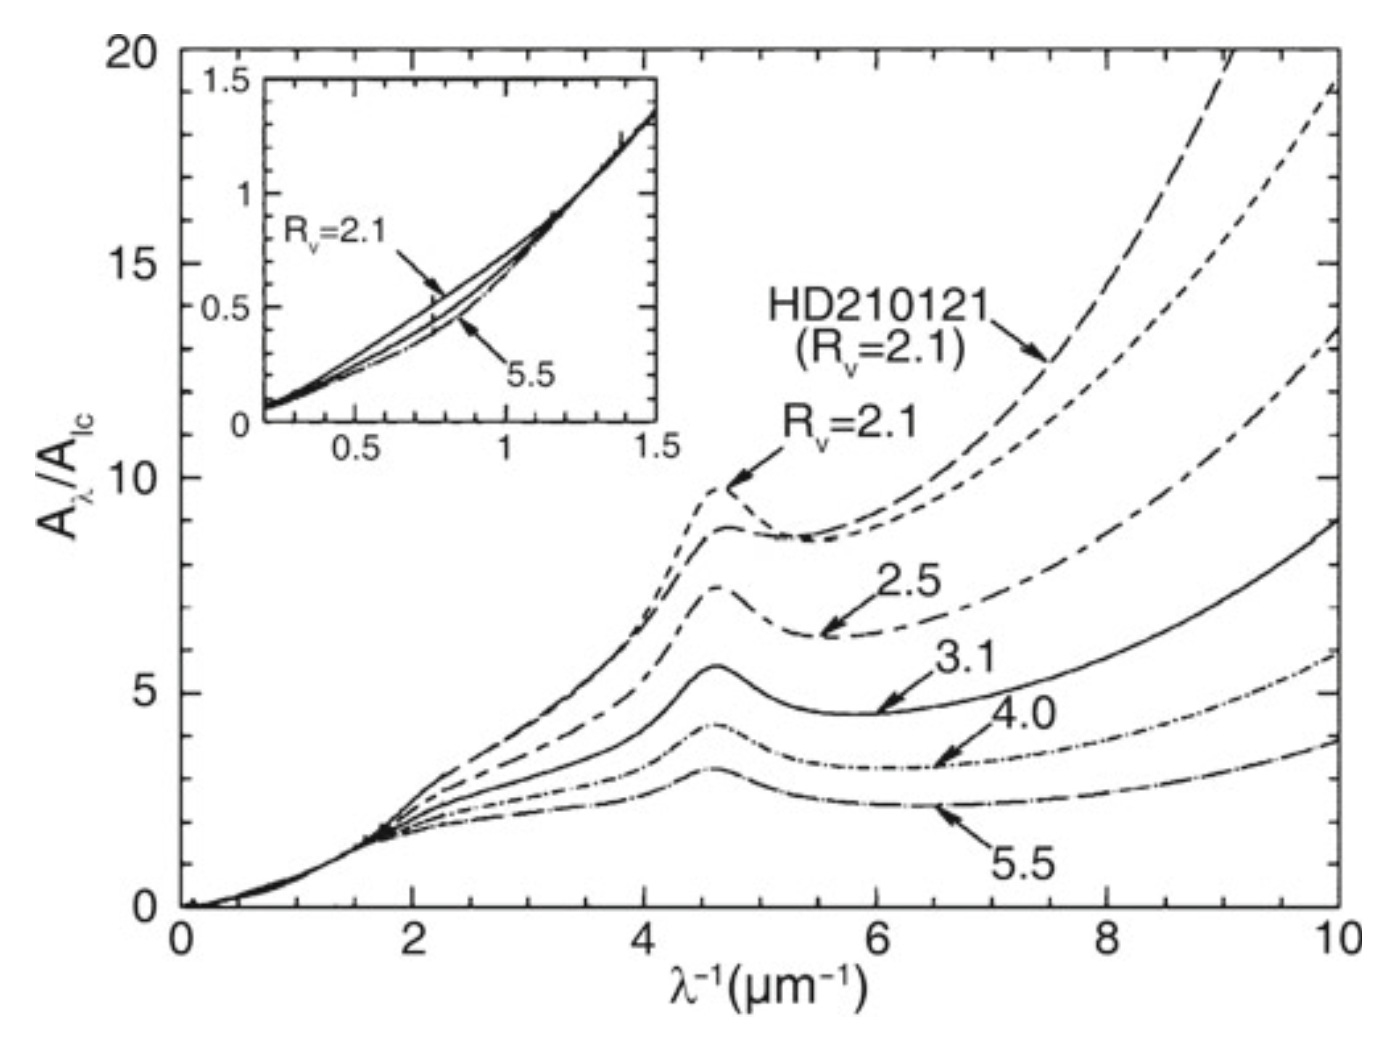
\includegraphics[width=12cm]{figures/ExtinctionCurve.png}}
\end{figure}

{\noindent}The extinction coefficient $A_V$ is proportional to the optical depth towards a source and so is the colour excess. Since the extinction is due to dust along the line-of-sight, the colour excess is proportional to the column density of dust towards the source. If we assume that the dust-to-gas ratio in the interstellar medium does not vary greatly, we expect that the column density of neutral hydrogen $N_\mathrm{H}$ is proportional to the colour excess. The former can be measured from the Lyman-$\alpha$ absorption in the spectra of stars, whereas the latter is obtained by comparing the observed colour of these stars with the colour expected for the type of star, given its spectrum (and thus, its spectral classification). One finds indeed that the color excess is proportional to the HI column density with

\begin{align*}
    E(B-V) = 1.7 \left(\frac{N_\mathrm{H}}{10^{22}\,{\rm atoms\,cm^{-2}}}\right) ~ [{\rm mag}],
\end{align*}

{\noindent}and a scatter of about 30\% around this relation. The fact that this scatter is so small indicates that the assumption of a constant dust-to-gas ratio is reasonable.

{\noindent}In the Solar neighborhood the extinction coefficient for sources in the disk is about

\begin{align*}
    A_V \approx \frac{d}{1\,{\rm kpc}} ~ [{\rm mag}],
\end{align*}

{\noindent}but this relation is at best a rough approximation, since the absorption coefficient can show strong local deviations from this law, for instance in the direction of molecular clouds.

{\noindent}\textbf{Colour-colour diagram}: As a first step in this measurement, it is necessary to determine the degree of extinction, which can only be done by analyzing the reddening. The stars of the cluster are plotted in a color-color diagram, for example by plotting the colors $(U-B)$ versus $(B-V)$. A colour-colour diagram also shows a main sequence along which the majority of the stars are aligned. The wavelength-dependent extinction causes a reddening in both colors. This shifts the positions of the stars in the diagram. The direction of the reddening vector depends only on the properties of the dust and is here assumed to be known, whereas the amplitude of the shift depends on the extinction coefficient. In a similar way to the CMD, this amplitude can now be determined if one has access to a calibrated, unreddened main sequence for the colour-colour diagram which can be obtained from the examination of nearby stars. From the relative shift of the main sequence in the two diagrams one can then derive the reddening and thus the extinction. The essential point here is the fact that the colour-colour diagram is \textit{independent of the distance}.

{\noindent}This then defines the procedure for the distance determination of a star cluster using photometry: in the first step we determine the reddening $E(B-V)$, and thus also $A_V$ via $A_V=(3.1\pm0.1)E(B-V)$ for the Galactic medium, by shifting the main sequence in a colour-colour diagram along the reddening vector until it matches a calibrated main sequence. In the second step the distance modulus is determined by vertically (i.e., in the direction of $M$) shifting the main sequence in the CMD until it matches a calibrated main sequence. From this, the distance is finally obtained according to

\begin{align*}
    m-M = 5\log\left(\frac{d}{1\,{\rm pc}}\right)-5+A ~ [{\rm mag}].
\end{align*}

{\noindent}\textbf{Spectroscopic distance}: From the spectrum of a star, the spectral type as well as its luminosity class can be obtained. The former is determined from the strength of various absorption lines in the spectrum, while the latter is obtained from the width of the lines. From the line width the surface gravity of the star can be derived, and from that its radius (more precisely, $M/R2^2$). The spectral type and the luminosity class specify the position of the star in the HRD unambiguously. By means of stellar evolution models, the absolute magnitude $M_V$ can then be determined. Furthermore, the comparison of the observed colour with that expected from theory yields the color excess $E(B-V)$, and from that we obtain $A_V$. With this information we are then able to determine the distance using

\begin{align*}
    m_V-A_V-M_V = 5\log\left(\frac{d}{1\,{\rm pc}}\right)-5 ~ [{\rm mag}].
\end{align*}

{\noindent}\textbf{Visual binaries}: Kepler’s third law for a two-body problem,

\begin{align*}
    P = \sqrt{\frac{4\pi^2}{G(m_1+m_2)}a^3} ~ [{\rm yr}]
\end{align*}

{\noindent}relates the orbital period $P$ of a binary star to the masses $m_i$ of the two components and the semi-major axis $a$ of the ellipse. The latter is defined by the separation vector between the two stars in the course of one period. This law can be used to determine the distance to a visual binary star. For such a system, the period $P$ and the angular diameter $2\theta$ of the orbit are direct observables. If one additionally knows the mass of the two stars, for instance from their spectral classification, $a$ can be determined according to Kepler's third law, and from this the distance follows with the small angle approximation $d=a/\theta$.

{\noindent}\textbf{Variable stars}: Several types of pulsating stars show periodic changes in their brightnesses, where the period of a star is related to its mass, and thus to its luminosity. This period-luminosity (PL) relation is ideally suited for distance measurements: since the determination of the period is independent of distance, one can obtain the luminosity directly from the period if the calibrated PL-relation is known. The distance is thus directly derived from the measured magnitude using the photometric distance, if the extinction can be determined from color measurements.

{\noindent}The existence of a relation between the luminosity and the pulsation period can be expected from simple physical considerations. Pulsations are essentially radial density waves inside a star that propagate with the speed of sound, $c_s$. Thus, one can expect that the period is comparable to the sound crossing time through the star, $P\sim R/c_s$. The speed of sound $c_s$ in a gas is of the same order of magnitude as the thermal velocity of the gas particles, so that $k_BT\sim m_pc_s^2$, where $m_p$ is the proton mass (and thus a characteristic mass of particles in the stellar plasma) and $k_B$ is Boltzmann's constant. According to the virial theorem, one expects that the gravitational binding energy of the star is about twice the kinetic (i.e., thermal) energy, so that for a proton,

\begin{align*}
    \frac{GMm_p}{R} \sim k_BT.
\end{align*}

{\noindent}Combining these relations, we obtain for the pulsation period

\begin{align*}
    P\sim\frac{R}{c_s}\sim\frac{R\sqrt{m_p}}{\sqrt{k_BT}} \sim\frac{R^{3/2}}{\sqrt{GM}} \propto \langle\rho\rangle^{-1/2},
\end{align*}

{\noindent}where $\langle\rho\rangle$ is the mean density of the star. This is a remarkable result -- the pulsation period depends only on the mean density. Furthermore, the stellar luminosity is related to its mass by approximately $L/M^3$. If we now consider stars of equal effective temperature $T_\mathrm{eff}$ (where $L\propto R^2T_\mathrm{eff}^4$), we find that

\begin{align*}
    P \propto \frac{R^{3/2}}{\sqrt{M}} \propto L^{7/12},
\end{align*}

{\noindent}which is the relation between period and luminosity that we were aiming for.

{\noindent}One finds that a well-defined period-luminosity relation exists for three types of pulsating stars:

\begin{itemize}
    \item $\boldsymbol{\delta}$ \textbf{Cepheid stars} (classical Cepheids): These are young stars found in the disk population (close to the Galactic plane) and in young star clusters.
    \item \textbf{W Virginis stars}: Also called population II Cepheids. These are low-mass, metal-poor stars located in the halo of the Galaxy, in globular clusters, and near the Galactic center.
    \item \textbf{RR Lyrae stars}: These are likewise population II stars and thus metal-poor. They are found in the halo, in globular clusters, and in the Galactic bulge.
\end{itemize}

{\noindent}\textbf{Globular clusters}: 

{\noindent}\textbf{Tully-Fisher relation}: Using $21\,{\rm cm}$ observations of spiral galaxies, in 1977 R. Brent Tully and J. Richard Fisher found that the maximum rotation velocity of spirals is closely related to their luminosity, following the relation

\begin{align*}
    L_\mathrm{TF} \propto v_\mathrm{max}^\alpha ~ [{\rm erg\,s^{-1}}],
\end{align*}

{\noindent}where the power-law index (i.e., the slope) of the Tully-Fisher relation is about $\alpha\sim4$. The larger the wavelength of the filter in which the luminosity is measured, the smaller the dispersion of the Tully-Fisher relation (see Figure \ref{fig:tullyfisher}). This is to be expected because radiation at larger wavelengths is less affected by dust absorption and by the current star formation rate, which may vary to some extent between individual spirals. Furthermore, it is found that the value of $\alpha$ increases with the wavelength of the filter: The Tully-Fisher relation is steeper in the red, which follows from the fact that more massive, or more luminous galaxies (i.e., those with larger $v_\mathrm{,ax}$) are redder. The dispersion of galaxies around this relation in the NIR (e.g., in the H-band) is about 10\%.

\begin{figure}[h]
\floatbox[{\capbeside\thisfloatsetup{capbesideposition={right,top},capbesidewidth=4cm}}]{figure}[\FBwidth]
{\caption{\footnotesize{The Tully-Fisher relation for galaxies in the Local Group (dots), in the Sculptor group (triangles), and in the M81 group (squares). The absolute magnitude is plotted as a function of the width of the $21\,{\rm cm}$ profile which indicates the maximum rotation velocity. Filled symbols represent galaxies for which independent distance estimates were obtained, either from RR Lyrae stars, Cepheids, or planetary nebulae. For galaxies represented by open symbols, the average distance of the respective group is used. The solid line is a fit to similar data for the Ursa-Major cluster, together with data of those galaxies for which individual distance estimates are available (filled symbols). The larger dispersion around the mean relation for the Sculptor group galaxies is due to the group’s extent along the line-of-sight. Source: M.J. Pierce \& R.B. Tully 1992, Luminosity-line width relations and the extragalactic distance scale. I-Absolute calibration, ApJ 387, 47, p. 51, Fig. 1. Image taken from Schneider (2006).}}
\label{fig:tullyfisher}}
{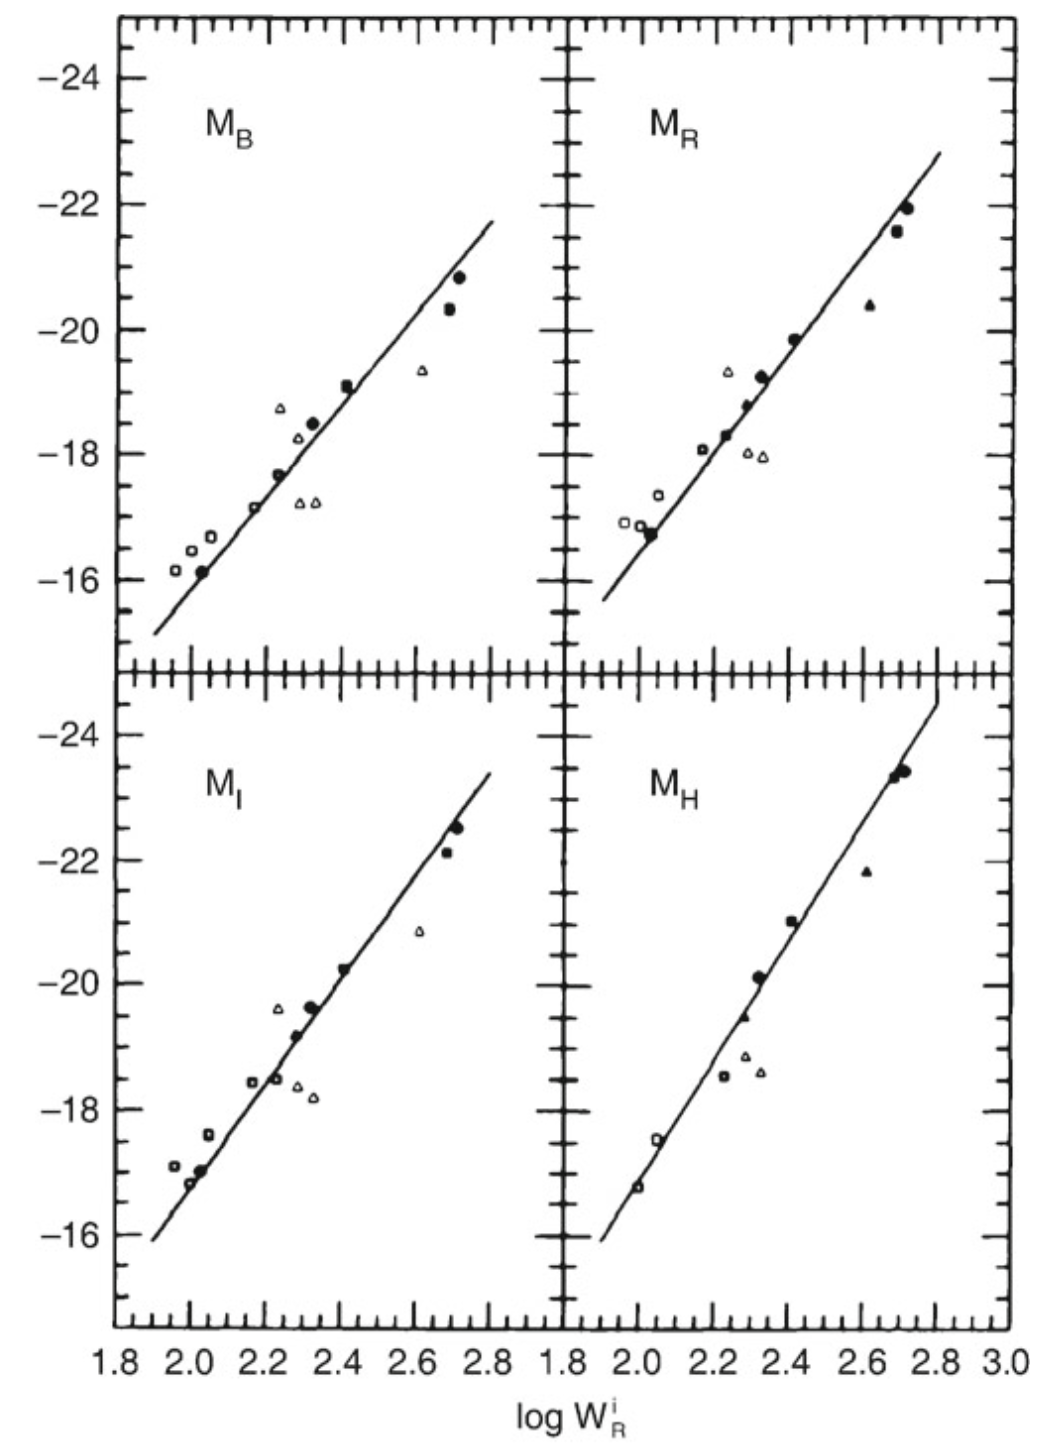
\includegraphics[width=10cm]{figures/TullyFisher.png}}
\end{figure}

{\noindent}Because of this close correlation, the luminosity of spirals can be estimated quite precisely by measuring the rotational velocity. The determination of the (maximum) rotational velocity is independent of the galaxy’s distance. By comparing the luminosity, as determined from the Tully-Fisher relation, with the measured flux, one can then estimate the distance of the galaxy -- without utilizing the Hubble relation!

{\noindent}The measurement of $v_\mathrm{max}$ is obtained either from a spatially resolved rotation curve, by measuring $v_\mathrm{rot}$, which can be done with optical spectroscopy or, for relatively nearby galaxies, also with spatially resolved $21\,{\rm cm}$ spectroscopy. Alternatively, one can observe an integrated spectrum of the $21\,{\rm cm}$ line of HI that has a Doppler width corresponding to about $2v_\mathrm{max}$ (see Fig.3.28). The Tully-Fisher relation shown in Figure \ref{fig:tullyfisher} was determined by measuring the width of the $21\,{\rm cm}$ line.

\begin{figure}[h]
    \floatbox[{\capbeside\thisfloatsetup{capbesideposition={right,top},capbesidewidth=4cm}}]{figure}[\FBwidth]
    {\caption{\footnotesize{$21\,{\rm cm}$ profile of the galaxy NGC7331. The bold dots indicate $20$ and $50$\% of the maximum flux; these are of relevance for the determination of the line width from which the rotational velocity is derived. Source: L.M. Macri et al. 2000, A Database of Tully-Fisher Calibrator Galaxies, ApJS 128, 461, p. 467, Fig. 5. Image taken from Schneider (2006).}}
    \label{fig:21cmvrot}}
    {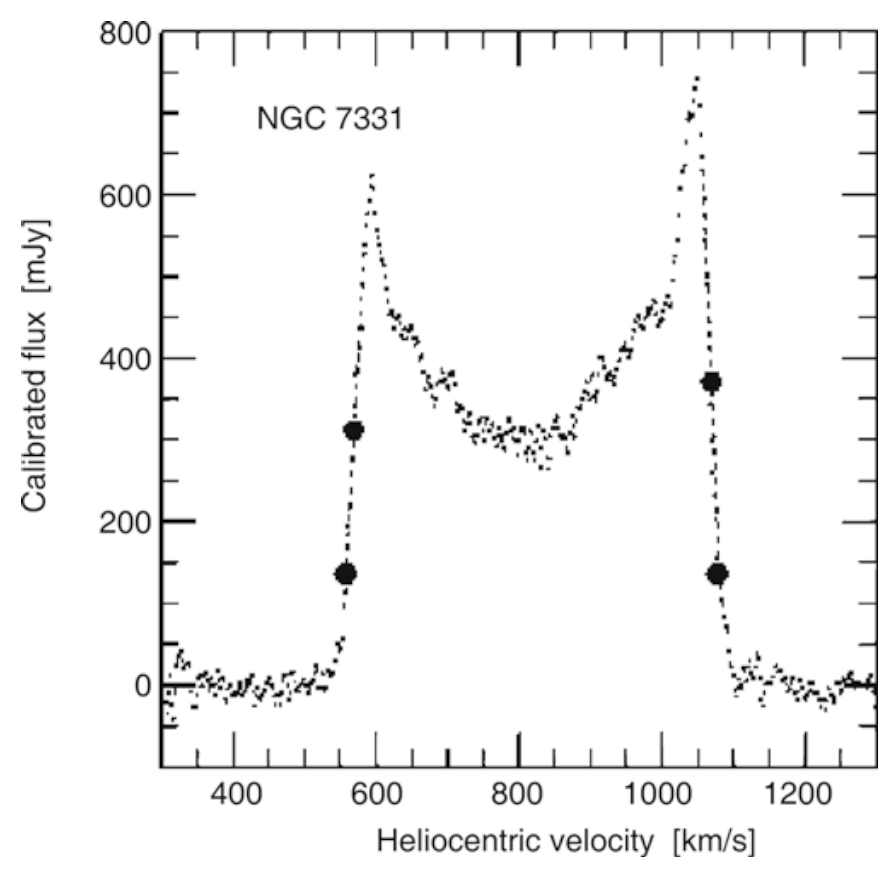
\includegraphics[width=8cm]{figures/21cm_vrot.png}}
\end{figure}

{\noindent}The shapes of the rotation curves of spirals are very similar to each other, in particular with regard to their flat behavior in the outer part. The flat rotation curve implies

\begin{align*}
    M = \frac{v_\mathrm{max}^2R}{G} ~ [{\rm M_\odot}],
\end{align*}

{\noindent}where the value of the distance $R$ from the center of the galaxy is chosen to be in the range of the flat part of the rotation curve (i.e., where $v_\mathrm{rot}(R)\approx v_\mathrm{max}$). We note that the exact value of $R$ is not important; of course, $M=M(R)$. By re-writing this,

\begin{align*}
    L = \left(\frac{M}{L}\right)^{-1} \frac{v_\mathrm{max}^2R}{G} ~ [{\rm erg\,s^{-1}}],
\end{align*}

{\noindent}and by replacing $R$ by the mean surface brightness $\langle I\rangle=L/R^2$, we obtain

\begin{align*}
    L = \left(\frac{M}{L}\right)^{-2} \left(\frac{1}{G^2\langle I\rangle}\right)v_\mathrm{max}^4 ~ [{\rm erg\,s^{-1}}].
\end{align*}

{\noindent}This is the Tully-Fisher relation if $M/L$ and $\langle I\rangle$ are the same for all spirals. The latter is in fact suggested by Freeman’s law. Since the shapes of rotation curves for spirals seem to be very similar, the radial dependence of the ratio of luminous to dark matter may also be quite similar among spirals. Furthermore, since the mass- to-light ratios of a stellar population as measured from the red or infrared emission do not depend strongly on its age, independently of their Hubble type. Within $R_{25}$ one finds $M/L_B=6.2$ for Sa's, $4.5$ for Sb's, and $2.6$ for Sc's. This trend does not come as a surprise because late types of spirals contain more young, blue and luminous stars.

{\noindent}\textbf{Faber-Jackson relation}: A relation for elliptical galaxies, analogous to the Tully-Fisher relation, was found by Sandra Faber and Roger Jackson. They discovered that the velocity dispersion in the center of ellipticals, $\sigma_v$, scales with luminosity,

\begin{align*}
    L_\mathrm{FJ} \propto \sigma_v^4 ~ [{\rm erg\,s^{-1}}]
\end{align*}

{\noindent}`Deriving' the Faber-Jackson scaling relation is possible under the same assumptions as for the Tully-Fisher relation. However, the dispersion of ellipticals about this relation is larger than that of spirals about the Tully-Fisher relation.

{\noindent}\textbf{$D_n-\sigma$ relation}: Another scaling relation for ellipticals which is of substantial importance in practical applications is the $D_n-\sigma$ relation. $D_n$ is defined as the mean diameter of an ellipse within which the average surface brightness. It corresponds to a value of $20.75\,{\rm mag\,arcsec^{-2}}$ in the B-band. If we now assume that all ellipticals have a self-similar brightness profile, $I(R)=I_ef(R/R_r)$, with $f(1)=1$, then the luminosity within $D_n$ can be written as

\begin{align*}
    I_n\left(\frac{D_n}{2}\right)^2\pi &= 2\pi I_e \int\limits_0^{D_n/2} Rf(R/R_e)\mathrm{d}R \\
    &= 2\pi I_eR_e^2 \int\limits_0^{D_n/(2R_e)} ~ [{\rm erg\,s^{-1}\,m^{-2}}] xf(x)\mathrm{d}x,
\end{align*}

{\noindent}where in the last step we changed the integration variable to $x=R/R_e$. For a de Vaucouleurs profile we have approximately $f(x)\propto x^{-1.2}$ in the relevant range of radius. Computing the integral with this expression, we obtain

\begin{align*}
    D_n \propto R_eI_e^{0.8}.
\end{align*}

{\noindent}Empirically, we find that ellipticals follow the normalized $D_n-\sigma$ relation

\begin{align*}
    D_n = 2.05\times\left(\frac{\sigma_v}{100\,{\rm km\,s^{-1}}}\right) ~ [{\rm kpc}]
\end{align*}

{\noindent}and they scatter around this relation with a relative width of about 15\%.

{\noindent}\textbf{Type Ia supernovae}: The \textbf{Phillips relation} is the empirical correlation between the peak luminosity of a Type Ia supernova and the speed of luminosity evolution after maximum light; the faster the supernova fades from maximum light, the fainter its peak magnitude was (i.e., slower-evolving light curves are found to have brighter maximum luminosities).


% --------------------------------------------------------------
%               4. 
% --------------------------------------------------------------

\newpage
\subsection{Question 4}

What evidence is there that most galaxies contain nuclear black holes? How do those black holes interact with their host galaxies?

\subsubsection{Short answer}

Evidence for most galaxies containing a SMBH includes: mass estimates using stellar orbital velocities in galaxy centers, strong non-thermal relativistic X-ray emission, and hypervelocity stars. Galaxies with a bulge component host a SMBH whose mass is tightly correlated with the properties of the stellar component suggesting that the SMBH evolves with its host galaxy. The BH directly affects their host galaxies through feedback processes. Accretion of material onto the SMBH powers a relativistic jet of material which can heat the surrounding gas and quench star formation. 

\subsubsection{Additional context}

The Milky Way harbors a black hole (BH) in its center. Furthermore, it is generally accepted that the energy for the activity of AGNs is generated by accretion onto a BH. Thus, the question arises as to whether all (or most) galaxies contain a super-massive black hole (SMBH) in their nuclei. Indeed, SMBHs are very abundant. This result then instigates further questions: what distinguishes a `normal' galaxy from an AGN if both have a SMBH in the nucleus? Is it the mass of the black hole, the rate at which matter is accreted onto it, or the efficiency of the mechanism which is generating the energy?

{\noindent}What is a BH? A technical answer is that a BH is the simplest solution of Einstein’s theory of general relativity which describes the gravitational field of a point mass. Less technically (though sufficient for our needs) we may say that a BH is a point mass, or a compact mass concentration, with an extent smaller than its Schwarzschild radius $r_S$.

{\noindent}The first discussion of BHs can be traced back to Laplace in 1795, who considered the following: if one reduces the radius $r$ of a celestial body of mass $M$, the \textbf{escape velocity} $v_\mathrm{esc}$ at its surface,

\begin{align*}
    v_\mathrm{esc} = \sqrt{\frac{2GM}{r}} ~ [{\rm km\,s^{-1}}],
\end{align*}

{\noindent}will increase. As a thought experiment, one can now see that for a sufficiently small radius, $v_\mathrm{esc}$ will be equal to the speed of light, $c$. This happens when the radius decreases to

\begin{align*}
    r_S \equiv \frac{2GM}{c^2} = 2.95\left(\frac{M}{{\rm M_\odot}}\right) ~ [{\rm km}].
\end{align*}

{\noindent}The radius $r_S$ is named the \textbf{Schwarzschild radius}, after Karl Schwarzschild who, in 1916, discovered the point-mass solution of Einstein's field equations. For our purpose we will define a BH as a mass concentration with a radius smaller than $r_S$. As we can see, $r_S$ is very small: about $3\,{\rm km}$ for the Sun, and $\sim10^{12}\,{\rm cm}$ for the SMBH in the Galactic center. At a distance of $R_0=8\,{\rm kpc}$, this corresponds to an angular radius of $\sim8\times10^{-6}\,{\rm arcsec}$. Current observing capabilities are still far from resolving scales of order $r_S$, except for the VLBI technique which currently comes close to it: the highest angular resolution currently achieved with millimeter-VLBI is a mere factor of $\sim10$ away from resolving the Schwarzschild radius for the Galactic BH that is supposed to coincide with the compact radio source Sgr A$^*$. By performing VLBI studies at sub-millimeter wavelengths in the near future, we may actually be able to `see' the Schwarzschild radius of a BH for the first time. The largest observed velocities of stars in the Galactic center,   $\sim5000\,{\rm km\,s^{-1}}\ll c$, indicate that they are still well away from the Schwarzschild radius. Relativistic effects are directly observed in AGNs and that velocities close to $c$ do in fact occur there -- which again is a very direct indication of the existence of a SMBH.

{\noindent}If even for the closest SMBH, the one in the GC, the Schwarzschild radius is significantly smaller than the achievable angular resolution, how can we hope to prove that SMBHs exist in other galaxies? Like in the GC, this proof has to be found indirectly by detecting a compact mass concentration incompatible with the mass concentration of the stars observed.

{\noindent}We consider a mass concentration of mass $M_\bullet$ in the center of a galaxy where the characteristic velocity dispersion of stars (or gas) is $\sigma_v$. We compare this velocity dispersion with the characteristic velocity (e.g., the Kepler rotational velocity) around a SMBH at a distance $r$, given by $\sqrt{GM_\bullet/r}$. From this it follows that, for distances smaller than

\begin{align*}
    r_\mathrm{BH} = \frac{GM_\bullet}{\sigma_v^2} \sim 0.4\left(\frac{M_\bullet}{10^6\,{\rm M_\odot}}\right)\left(\frac{\sigma_v}{100\,{\rm km\,s^{-1}}}\right)^{-2} ~ [{\rm pc}],
\end{align*}

{\noindent}the SMBH will significantly affect the kinematics of stars and gas in the galaxy. The corresponding angular scale is

\begin{align*}
    \theta_\mathrm{BH} = \frac{r_\mathrm{BH}}{d} \sim 0.1\left(\frac{M_\bullet}{10^6\,{\rm M_\odot}}\right) \left(\frac{\sigma_v}{100\,{\rm km\,s^{-1}}}\right)^{-2} \left(\frac{d}{1\,{\rm Mpc}}\right)^{-1} ~ [{\rm arcsec}],
\end{align*}

{\noindent}where $d$ is the distance of the galaxy. From this we immediately conclude that our success in finding SMBHs will depend heavily on the achievable angular resolution. The HST enabled scientists to make huge progress in this field. The search for SMBHs promises to be successful only in relatively nearby galaxies. In addition, we can see that for increasing distance $d$ the mass $M$  has to increase for a SMBH to be detectable at a given angular resolution.

{\noindent}The presence of a SMBH inside $r_\mathrm{BH}$ is revealed by an increase in the velocity dispersion for $r<r_\mathrm{BH}$, which should then behave as  $\sigma_v\propto r^{-1/2}$ for $r\lesssim r_\mathrm{BH}$. If the inner region of the galaxy rotates, one expects, in addition, that the rotational velocity $v_\mathrm{rot}$ should also increase inwards $\propto r^{-1/2}$.

\begin{figure}[t]
    \floatbox[{\capbeside\thisfloatsetup{capbesideposition={right,top},capbesidewidth=4cm}}]{figure}[\FBwidth]
    {\caption{\footnotesize{An HST image of the nucleus of the galaxy M84 is shown in the left-hand panel and the spectrum of the central region on the right. The position along the slit is plotted vertically with the relative wavelength change of the light horizontally. This shows the Kepler rotation in the central gravitational field of a SMBH, whose mass can be estimated as $M_\bullet \sim 3\times10^8\,{\rm M_\odot}$. Credit: Gary Bower, Richard Green (NOAO), the STIS Instrument Definition Team, and NASA/ESA. Image taken from Schneider (2006).}}
    \label{fig:m84hst}}
    {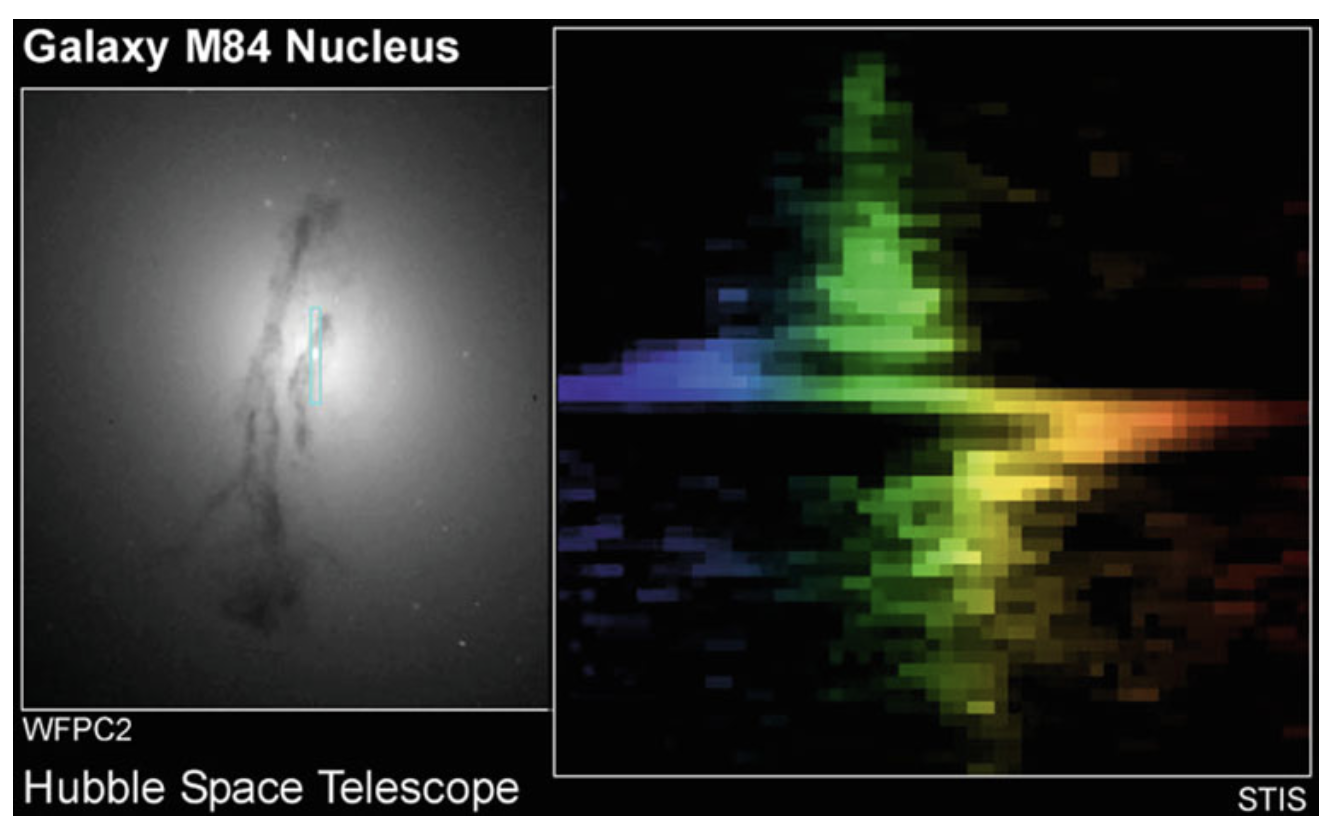
\includegraphics[width=10cm]{figures/M84HST.png}}
\end{figure}

{\noindent}The practical problems in observing a SMBH have already been mentioned above. One problem is the angular resolution. To measure an increase in the velocities for small radii, the angular resolution needs to be better than $\theta_\mathrm{BH}$. Furthermore, projection effects play a role because only the velocity dispersion of the projected stellar distribution, weighted by the luminosity of the stars, is measured. Added to this, the kinematics of stars can be rather complicated, so that the observed values for $\sigma_v$ and $v_\mathrm{rot}$ depend on the distribution of orbits and on the geometry of the distribution.

{\noindent}Despite these difficulties, the detection of SMBHs has been achieved in recent years, largely due to the much improved angular resolution of optical telescopes (like the HST) and to improved kinematic models. Black hole masses were determined for more than $70$ nearby galaxies, and upper limits on $M_\bullet$ were obtained for about $30$ galaxies.

{\noindent}Figure \ref{fig:m84hst} shows an example for the kinematical method discussed in the previous section. A long-slit spectrum across the nucleus of the galaxy M84 clearly shows that, near the nucleus, both the rotational velocity (seen by the mean wavelength of the emission line) and the velocity dispersion (given by the width of the line) change; both increase dramatically towards the center.

{\noindent}Currently, strong indications for SMBHs have been found in the kinematics of stars or gas, resolving the sphere of influence of the black hole, in more than $70$ nearby galaxies, and their masses have been estimated. This permits us to examine whether, and in what way, $M_\bullet$ is related to the properties of the host galaxy. In this way, a remarkable correlation was discovered: one finds that $M_\bullet$ is correlated with the absolute magnitude of the bulge component (or the spheroidal component) of the galaxy in which the SMBH is located (see Figure \ref{fig:bhcorrelations}, upper left panel). Here, the bulge component is either the bulge of a spiral or $S0$ galaxy or an elliptical galaxy as a whole. This correlation is described by

\begin{align*}
    M_\bullet = 1.7\times10^9\left(\frac{L_\mathrm{V}}{10^{11}\,{\rm L_{V_\odot}}}\right)^{1.11} ~ [{\rm M_\odot}],
\end{align*}

{\noindent}and indicated by the dotted line in the upper left panel of Figure \ref{fig:bhcorrelations}. The correlation is statistically highly significant, but the deviations of the data points from this power law are considerably larger than their error bars, with a scatter of about a factor $3$ at high luminosities, increasing towards fainter galaxies. Instead of the bulge luminosity, one can also study the correlation of $M_\bullet$ with the mass of the bulge, which is plotted in the upper right panel of Figure \ref{fig:bhcorrelations}, and for which the best power-law fit

\begin{align*}
    M_\bullet = 2.9\times10^8\left(\frac{M_\mathrm{bulge}}{10^11\,{\rm M_\odot}}\right)^{1.05} ~ [{\rm M_\odot}]
\end{align*}

{\noindent}is obtained. For the $M_\bullet(M_\mathrm{bulge})$ relation, the scatter is slightly smaller than around the $M_\bullet(L_\mathrm{V})$ relation. Given that the power-law index in the latter is almost unity, we can rewrite this relation in the form

\begin{align*}
    M_\bullet \approx 3\times10^{-3}M_\mathrm{bulge}.
\end{align*}

{\noindent}Thus we find that the BH mass is strongly correlated with the stellar properties of the host galaxy, and that the ratio of black hole mass and bulge mass is approximately $1/300$. In other words, 0.3\% of the baryon mass that was used to make the stellar population in the bulge of these galaxies was transformed into a central black hole.

{\noindent}An even tighter correlation exists between $M_\bullet$ and the velocity dispersion in the bulge component, as can be seen in the lower panel of Figure \ref{fig:bhcorrelations}. This relation is best described by

\begin{align*}
    M_\bullet = 2.1\times 10^8\left(\frac{\sigma_v}{200\,{\rm km\,s^{-1}}}\right)^{5.64} ~ [{\rm M_\odot}].
\end{align*}

\begin{figure}[t!]
    \centering
    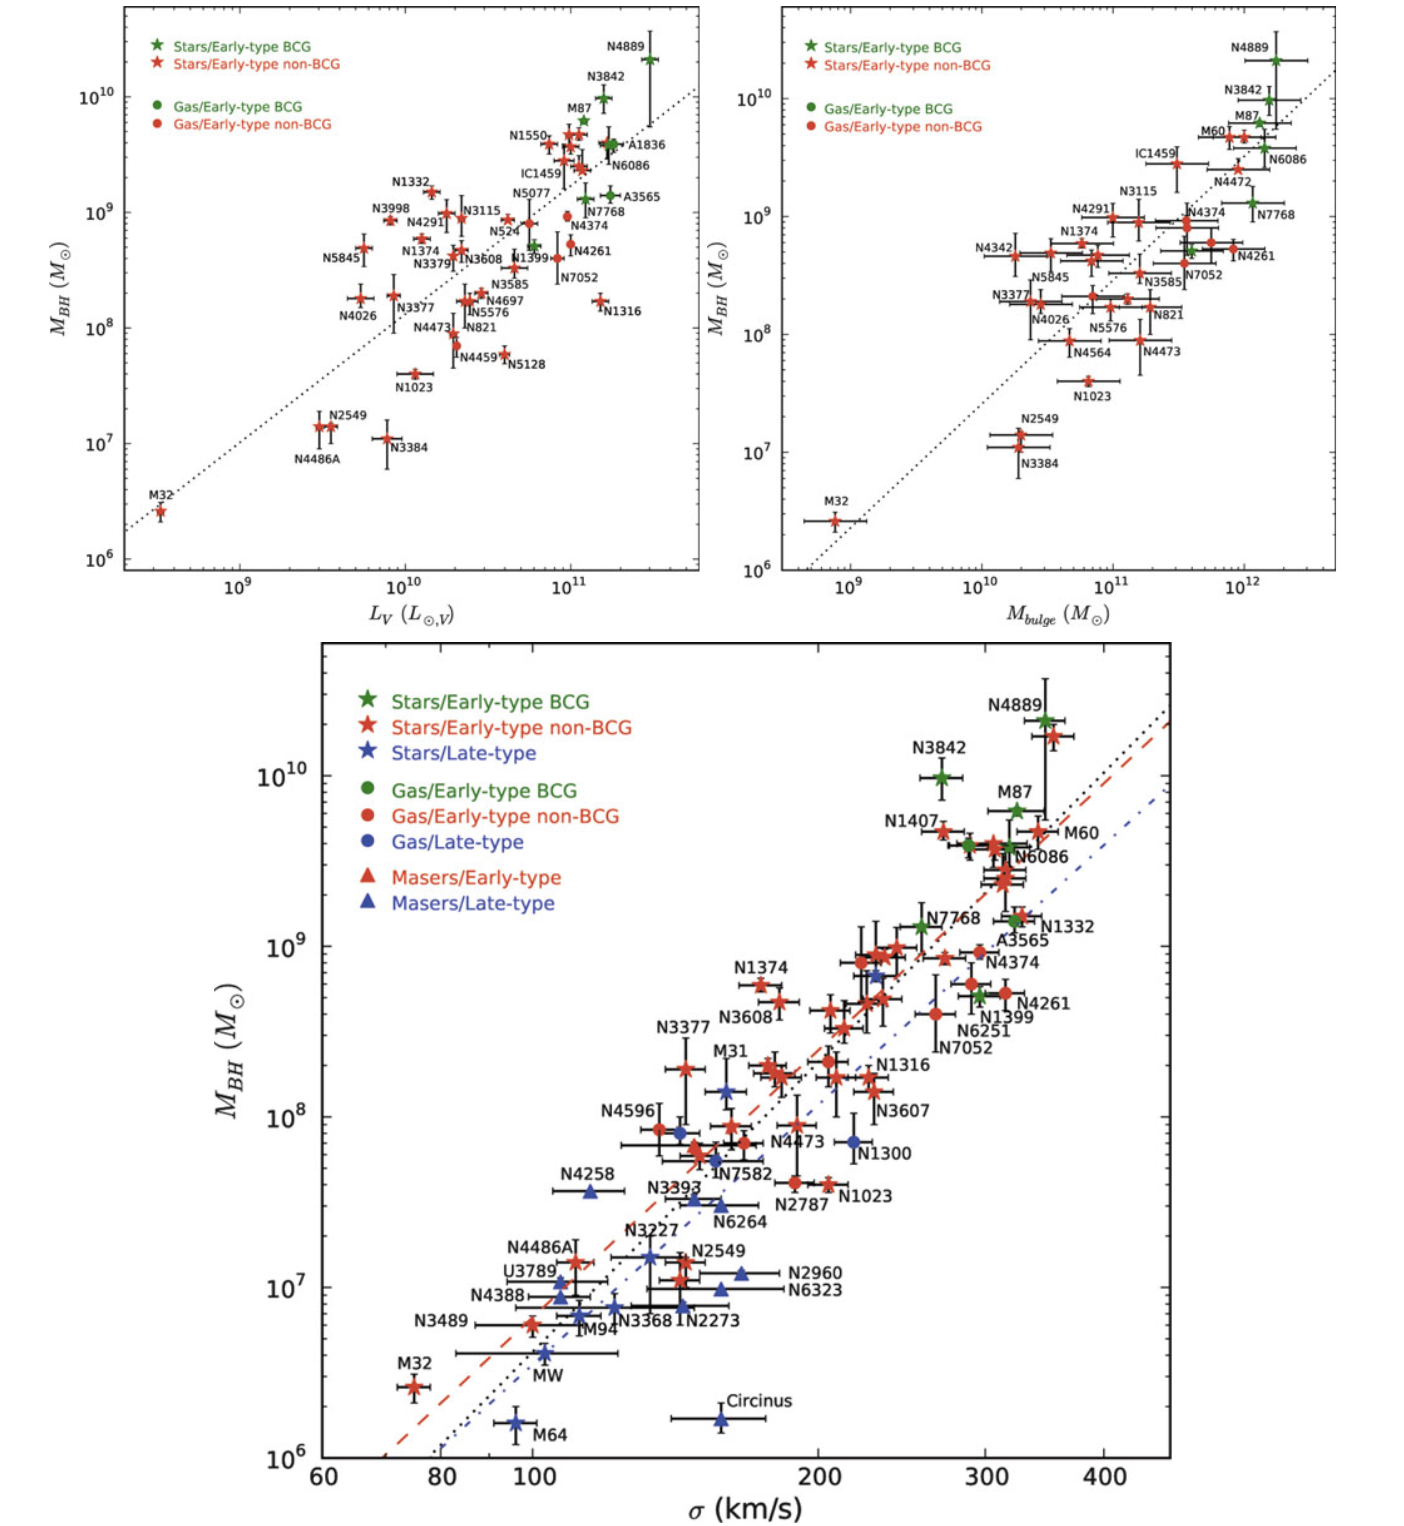
\includegraphics[width=15cm]{figures/BHcorrelations.png}
    \caption{\footnotesize{Black hole mass scaling relations, based on measurements of $M_\bullet$ in $72$ nearby galaxies. The upper left panel shows $M_\bullet$ as a function of the optical luminosity of the bulge component for early-type galaxies with reliable photometry. In the upper right panel, $M_\bullet$ is plotted as a function of the bulge stellar mass, as obtained from dynamical measurements. Finally, the lower panel shows $M_\bullet$ versus the velocity dispersion of the spheroidal component for the full sample of $72$ galaxies. Symbols indicate the methods with which $M_\bullet$ was determined : star-like symbols—stellar dynamics; circles—gas dynamics; triangles—masers. The color of the symbols indicate the galaxy type: green -- early type brightest cluster galaxy (BCG); red -- other early-type galaxies; blue -- late-type galaxies. The lines in the different panels correspond to power-law fits of the various scaling relations. Source: N.J. McConnell \& C.-P. Ma 2013, Revisiting the Scaling Relations of Black Hole Masses and Host Galaxy Properties, ApJ 764, 184, Figs. 1, 2 \& 3. AAS. Image taken from Schneider (2006).}}
    \label{fig:bhcorrelations}
\end{figure}

{\noindent}Fitting early- and late-type galaxies separately (shown by the red and blue lines in the bottom panel of Figure \ref{fig:bhcorrelations}), the slope of the scaling relation becomes slightly flatter ($5.2$ and $5.06$, respectively), with a normalization for the early-type galaxies being larger by about a factor $2$ than that for late-type galaxies. Since the velocity dispersion in late-type galaxies is smaller than that for early-types, the difference in the normalization of the $M_\bullet(\sigma_v)$ relation between these two galaxy populations is responsible for the steeper slope of the combined power-law fit. The scatter of the $M_\bullet(\sigma_v)$ relation is smaller than those of the scaling relations with mass and luminosity, about a factor of $2.5$, and the scatter decreases slightly with increasing  $\sigma_v$.

{\noindent}Hence we conclude that galaxies with a bulge component host a SMBH, whose mass is tightly correlated with the properties of the stellar component; in particular, the BH mass amounts to about 0.3\% of the stellar mass in the bulge component.

{\noindent}There have been claims in the literature that even globular clusters contain a BH; however, these claims are not undisputed. In addition, there may be objects that appear like globular clusters, but are in fact the stripped nucleus of a former dwarf galaxy. In this case, the presence of a central BH is not unexpected, provided the scaling relations holds down to very low velocity dispersion.

{\noindent}To date, the physical origin of this very close relation has not been understood in detail. The most obvious apparent explanation (that in the vicinity of a SMBH with a very large mass the stars are moving faster than around a smaller-mass SMBH) is not correct: the mass of the SMBH is significantly less than one percent of the mass of the bulge component. This is in contrast to the previously discussed case where the kinematics of the stars and gas were measured within the sphere of influence -- but the size of this is much smaller than the bulge component itself. We can therefore disregard the contribution of the SMBH to the gravitational field in which the stars are orbiting, except in the very inner region. Instead, this correlation has to be linked to the fact that the spheroidal component of a galaxy evolves together with the SMBH. A better understanding of this relation can only be found from models of galaxy evolution.

{\noindent}For very massive halos, the suppression of cooling flows in galaxy clusters is due to AGN activity of the central galaxy in the cluster. Since (almost) all massive galaxies contain a SMBH, this kind of feedback may be operational not only in groups and clusters, but actually in individual massive galaxies as well. In particular, there is a great deal of evidence for a relation between nuclear starbursts in galaxies and AGN activity. The gas needed for a starburst in the center of a galaxy is also potential fuel for the central BH. The details of this process are quite uncertain, but with plausible prescriptions, the cut-off of the luminosity function at $L\gtrsim L^*$ can be successfully modeled.

{\noindent}Feedback by an AGN can occur in several ways. In the case of galaxy clusters, the major effect of the AGN is the insertion of hot bubbles into the ICM through radio jets. The AGNs in most central cluster galaxies are not very luminous, and seem to be in the `radio mode' of low accretion rate. Thus, for low accretion rates, the main channel of feedback is the injection of mechanical energy into the surrounding gas. At high accretion rates, in the `quasar mode', the main source of feedback is presumably heating of the gas. Furthermore, the strong radiation field from quasars changes the ionization structure of the surrounding gas, which affects its cooling curve and at low temperatures actually leads to radiative heating.

\subsubsection{Follow-up Questions}

\begin{itemize}
    \item Does heating from AGN affect star formation in the outer parts of the disk?
    \item How are SMBHs formed?
    \item How are properties of SMBHs and their host galaxies related?
\end{itemize}

% --------------------------------------------------------------
%               5. 
% --------------------------------------------------------------

\clearpage
\subsection{Question 5}

Define and describe globular clusters. Where are they located? What are their typical ages, and how is this determined?

\subsubsection{Short answer}

Globular clusters are much more massive stellar systems, containing $10^4-10^6$ stars in a nearly spherical distribution located within the galactic halo. Globular clusters do not contain gas, dust, or young stars. The stellar density in the center of a globular cluster is extremely high: a typical value is $10^4\,{\rm M_\odot pc^{-3}}$, compared with $0.05\,{\rm M_\odot pc^{-3}}$ in the solar neighborhood. Most globular clusters are at a distance of $r\lesssim35\,{\rm kpc}$ (with $r=\sqrt{R^2+z^2}$) from the Galactic center, but some are also found at $r>60\,{\rm kpc}$. At these distances it is hard to judge whether these objects are part of the Galaxy or whether they have been captured from a neighboring galaxy, such as the Magellanic Clouds. Their typical ages are $\sim10\,{\rm Gyrs}$ which is determined using their main sequence turnoff point.

\subsubsection{Additional context}

Our Galaxy contains about $150$ globular clusters, but large elliptical galaxies such as M87 can contain as many as $10,000$. It is a mystery why young globular clusters are largely absent in our Galaxy but common in many others, such as M31, the Large Magellanic Cloud, and galaxies that have undergone recent mergers. Unlike open clusters, the Galaxy's globular clusters are old, and are believed to be relics of the formation of the Galaxy itself. The metallicity appears to be the same for all the stars in a given cluster (presumably because the cluster formed from a well-mixed gas cloud) but different clusters have a wide range of metallicity, from only $0.005\,{\rm Z_\odot}$ to nearly solar. The spatial distribution and the kinematics of a group of clusters are correlated with the metallicity, and for many purposes the clusters in our Galaxy can be divided into two groups: a roughly spherical population that contains 80\% of the clusters, shows little or no rotation and has metallicity $Z<0.1\,{\rm Z_\odot}$, and is associated with the stellar halo; and a flattened population that contains the remaining 20\%, has $Z>0.1\,{\rm Z_\odot}$, exhibits rapid rotation, and is associated with the disk and bulge. This bimodal distribution of metallicities is present in the globular cluster systems of other galaxies as well.

{\noindent}Because globular clusters have strong or high central concentration (the central density is much larger than the mean density) three different measures of the radius are usually quoted for globular clusters: the core radius, where the surface brightness has fallen to half its central value; the median or half-light radius, the radius of a sphere that contains half of all the luminosity; and the limiting or tidal radius, the outer limit of the cluster where the density drops to zero. Typical values of these and other cluster parameters are given in Table \ref{table:globularclusterstable}.

\begin{table}[h!]
    \centering
    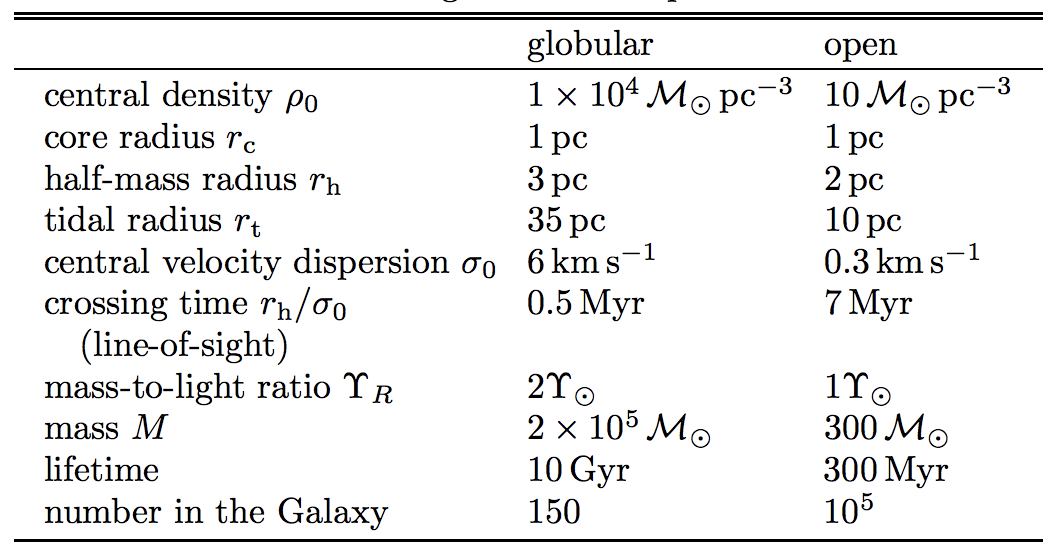
\includegraphics[width=10cm]{figures/GlobularClustersTable.png}
    \caption{\footnotesize{Parameters of globular and open clusters. Values for globular clusters are medians from the compilation of Harris (1996). Values for open clusters are from Figure 8.5, Piskunov et al. (2007), and other sources. Table taken from Binney \& Tremaine (2008).}}
    \label{table:globularclusterstable}
\end{table}

{\noindent}The visible halo of our Galaxy consists of about 150 globular clusters and field stars with a high velocity component perpendicular to the Galactic plane. Even at about 150, the number of known globular clusters is relatively small. A globular cluster is a collection of typically several hundred thousand stars, contained within a spherical region of radius $\sim20\,{\rm pc}$. The stars in the cluster are gravitationally bound and orbit in the common gravitational field. The old globular clusters with $[Fe/H]<-0.8$ have an approximately spherical distribution around the Galactic center. A second population of globular clusters exists that contains younger stars with a higher metallicity, $[Fe/H]>-0.8$. They have a more oblate geometrical distribution and are possibly part of the thick disk because they show roughly the same scale-height.

{\noindent}The density distribution of metal-poor globular clusters and field stars in the halo is described by

\begin{align*}
    n(r)\propto r^{-\gamma} ~ [{\rm Mpc^3}],
\end{align*}

{\noindent}with a slope $\gamma$ in the range $3-3.5$.

\begin{figure}[t]
    \floatbox[{\capbeside\thisfloatsetup{capbesideposition={right,top},capbesidewidth=4cm}}]{figure}[\FBwidth]
    {\caption{\footnotesize{A schematic side view of the Milky Way. Figure taken from Sparke (2007)}}
    \label{fig:mwgschematic}}
    {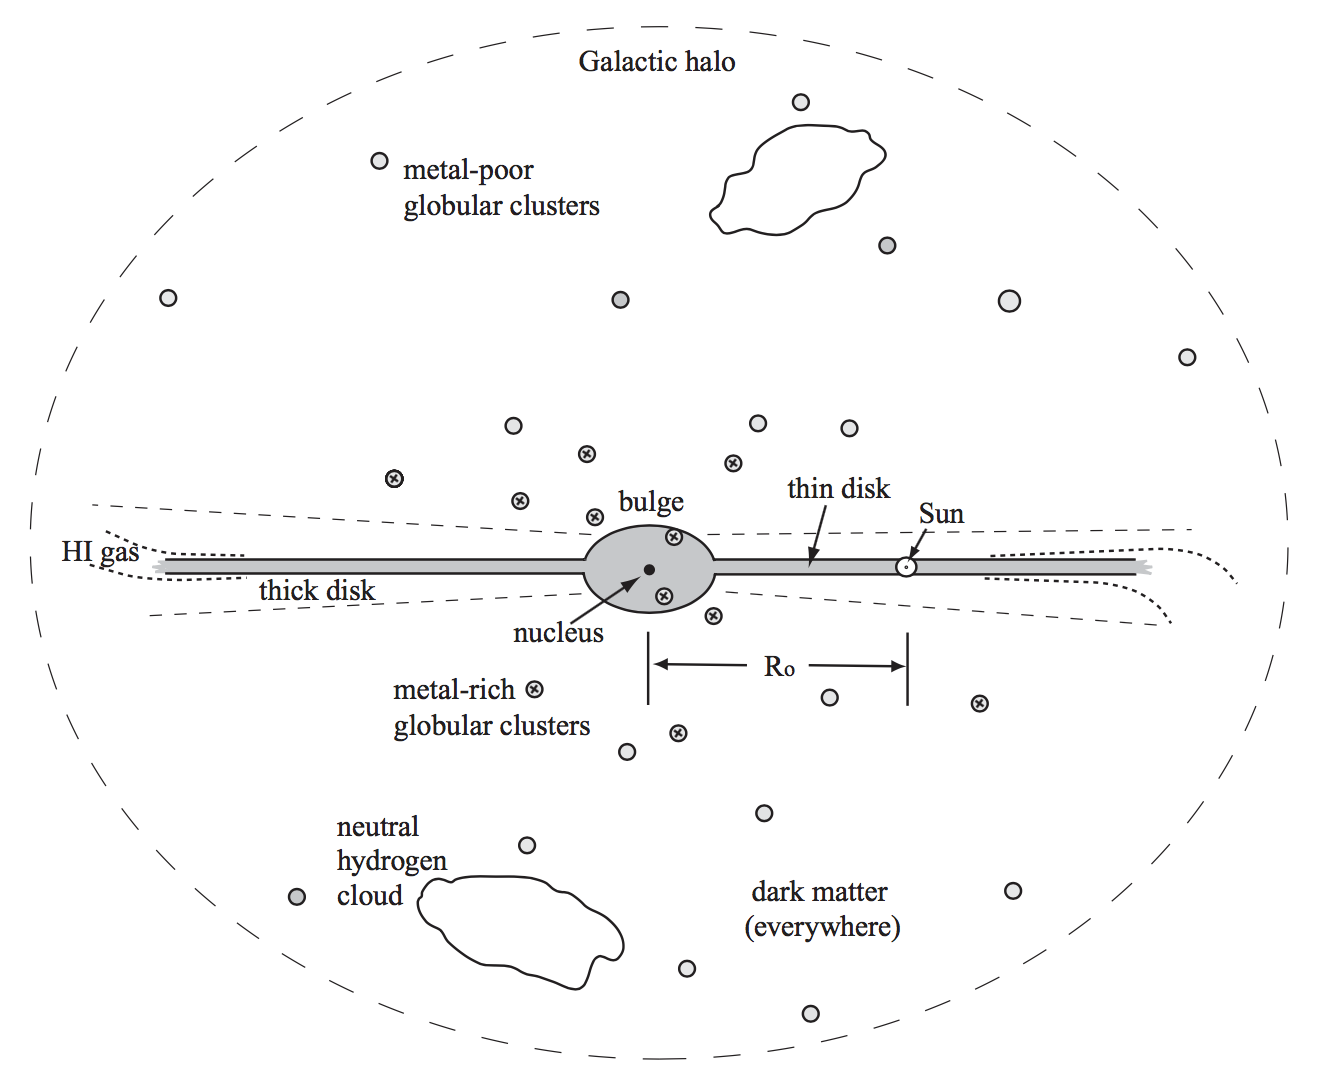
\includegraphics[width=10cm]{figures/MWGschematic.png}}
\end{figure}

{\noindent}The number of globular clusters is higher in early types and in more luminous galaxies. The specific abundance of globular clusters in a galaxy is defined as their number, normalized to a galaxy of absolute magnitude $M_V=-15$. This can be done by scaling the observed number $N_t$ of globular clusters in a galaxy of visual luminosity $L_V$ or absolute magnitude $M_V$, respectively, to that of a fiducial galaxy with $M_V$ corresponding to a luminosity of $L_V=L_{15}$:

\begin{align*}
    S_N = N_t\frac{L_{15}}{L_V} = N_t10^{0.4(M_V+15)} ~ [{\rm dimensionless}].
\end{align*}

{\noindent}If the number of globular clusters were proportional to the luminosity (and thus roughly to the stellar mass) of a galaxy, then this would imply a constant $S_N$ . However, this is not the case: For Sa's and Sb's we find $S_N\sim1.2$, whereas $S_N\sim0.5$ for Sc's. $S_N$ is larger for ellipticals and largest for cD galaxies.

{\noindent}There have been claims in the literature that even globular clusters contain a black hole; however, these claims are not undisputed. In addition, there may be objects that appear like globular clusters, but are in fact the stripped nucleus of a former dwarf galaxy. In this case, the presence of a central black hole is not unexpected.

{\noindent}Historically, measuring globular cluster (GC) ages has been a major driver to refine stellar evolution models and bring them to the best possible state of the art. The same applies to GC observations, both photometrically (especially with HST) and spectroscopically, thus submitting stellar models to more and more stringent observational checks. Indeed, with GC ages a strict lower limit on the age of the Universe was at stake, and for quite some time in the 1980s they have been an embarrassment for the young, matter dominated Universe many were advocating at the time. Indeed, GC ages contributed to keeping open the door to a cosmological constant (or some equivalent to it) prior to the unambiguous discovery of the universal acceleration. Now, at the time of the precision/concordance cosmology, the age of the Universe issue appears to be solved, and as a side benefit we can be quite confident on the reliability of stellar evolution models, that never indicated GC ages significantly below 12 Gyr.

{\noindent}The mainstream method to measure absolute globular cluster ages relies of the relation between the luminosity of the main sequence turnoff of theoretical isochrones, the age, and chemical composition. In turn, the absolute visual magnitude of the turnoff is given by $m_\mathrm{TO} - M_\mathrm{TO} = 5\log(d)-5$, where $m_\mathrm{TO}$ (the turnoff apparent magnitude corrected for extinction) is the directly observable quantity.


\subsubsection{Follow-up Questions}

\begin{itemize}
    \item Can you say something about collisional behavior in clusters?
    \item Why do or don't we think globular clusters have dark matter? How would we determine this? 
\end{itemize}

% --------------------------------------------------------------
%               6. 
% --------------------------------------------------------------

\newpage
\subsection{Question 6}

Describe three different methods used in the determination of the mass of a galaxy cluster.

\subsubsection{Short answer}

{\noindent}\textbf{Virial equilibrium}: Assuming the number of galaxies is large and are in virial equilibrium, the mass can be estimated via the virial mass.

{\noindent}\textbf{X-ray gas}: This gas temperature is a measure for the depth of the cluster's potential well, since the hotter the gas is, the deeper the potential well has to be to prevent the gas from escaping via evaporation.

{\noindent}\textbf{Gravitational lensing}: Utilizes the fact that light is deflected in a gravitational field. The angle through which light rays are bent due to the presence of a massive object depends on the mass of that object.

\subsubsection{Additional context}

{\noindent}\textbf{Virial equilibrium}: The time-averaged kinetic and potential energies are related by

\begin{align*}
    \frac{1}{2} \left\langle\frac{{\rm d^2}I}{{\rm d}t^2}\right\rangle - 2\langle K\rangle = \langle U\rangle,
\end{align*}

{\noindent}where $I$ is the region's moment of inertia. If the galaxy cluster is in equilibrium, then $\langle{\rm d}^2I/{\rm d}t^2\rangle$=0, resulting in the usual statement of the virial theorem:

\begin{align*}
    -2\langle K\rangle = \langle U\rangle.
\end{align*}

{\noindent}Furthermore, for a large number of galaxies, the galaxy cluster will look the same (in a statistical sense) at any time, and the time-averaging can be dropped. So for $N$ galaxies, 

\begin{align*}
    -2\sum_{i=1}^N \frac{1}{2}m_iv_i^2 = U,
\end{align*}

{\noindent}where $U$ is the total potential energy given by

\begin{align*}
    \sum_i \vec{F}_i\cdot\vec{r}_i = -\frac{1}{2}\sum_i\sum_{j\neq i} G\frac{m_im_j}{r_{ij}} = \frac{1}{2}\sum_i\sum_{j\neq i}U_{ij} = U.
\end{align*}

{\noindent}For simplicity, we restrict our attention to a spherical cluster of radius $R$ with $N$ galaxies, each of mass $m$, so the total mass of the galaxy cluster is $M=Nm$. Dividing the above expression by $N$ produces

\begin{align*}
    -\frac{m}{N}\sum_{i=1}^Nv_i^2 = \frac{U}{N}.
\end{align*}

{\noindent}Of course, astronomers actually measure the radial component of the velocity vector (galaxies are too far away to allow for detection of proper motions). Moreover, an astronomer is just as likely to see a star moving in the radial direction as in either of the two other perpendicular directions. With the brackets denoting an average value,

\begin{align*}
    \langle v^2\rangle = \langle v_r^2\rangle + \langle v_\theta^2\rangle + \langle v_\phi^2\rangle = 3\langle v_2^2\rangle,
\end{align*}

{\noindent}so,

\begin{align*}
    \frac{1}{N}\sum_{i=1}^Nv_i^2 = \langle v^2\rangle = 3\langle v_r^2\rangle = 3\sigma_r^2,
\end{align*}

{\noindent}where $\sigma_r$ is the dispersion in the radial velocity. Inserting this result into our equation for $U/N$, and using

\begin{align*}
    U \sim -\frac{16\pi^2}{15}G\bar{\rho}^2R^5 \sim -\frac{3}{5}\frac{GM^2}{R}
\end{align*}

for the approximate potential energy of a spherical distribution of total mass $M$ and radius $R$, leads to

\begin{align*}
    -3m\sigma_r^2 \approx -\frac{3}{5}\frac{GM^2}{NR}.
\end{align*}

{\noindent}Using $M=Nm$ and solving for mass gives

\begin{align*}
    M_{\rm vir} \approx \frac{5R\sigma_r^2}{G},
\end{align*}

{\noindent}where the mass obtained in this way is called the virial mass.

{\noindent}\textbf{Hot intracluster X-ray gas}: A portion of Zwicky's ``missing mass'' was discovered with the High Energy Astronomical Observatory (HEAO) series of satellites that were first launched in 1977. They revealed that many clusters of galaxies emit X-rays from much of the cluster's volume. These satellites, together with optical observations, indicated that clusters of galaxies contain an intracluster medium. The intracluster medium has two components. One is a diffuse, irregular distribution of stars. The other component is a hot intracluster gas that is distributed more or less homogeneously, occupying the space between the galaxies and filling the cluster's gravitational well. This gas temperature is a measure for the depth of the cluster's potential well, since the hotter the gas is, the deeper the potential well has to be to prevent the gas from escaping via evaporation. The X-ray luminosities lie in the range of $10^{36}$ to $10^{38}\,{\rm W}$, with richer clusters shining more brightly in X-rays. Typically, the mass of the gas is several times greater than the combined mass of all stars in the cluster's galaxies.

{\noindent}Thermal bremsstrahlung, the same mechanism that produces X-rays from the hot gas within individual galaxies, is at work here as well. For fully ionized hydrogen gas, the energy emitted per unit volume per unit time between frequencies $\nu$ and $\nu+{\rm d}\nu$ is given by

\begin{align*}
    \ell_\nu{\rm d}\nu = 5.44\times10^{-52}(4\pi n_e^2) T^{-1/2} e^{-h\nu/k_BT}{\rm d}\nu ~ [{\rm W\,m^{-3}}],
\end{align*}

{\noindent}where $T$ is the gas temperature and $n_e$ is the number density of free electrons. The total amount of energy emitted per second per unit volume at all frequencies (i.e., the luminosity density) is obtained by integrating $\ell_\nu$ over frequency. This results in

\begin{align*}
    \mathcal{L}_{\rm vol} = 1.42\times10^{-40}n_e^2T^{1/2} ~ [{\rm W\,m^{-3}}].
\end{align*}

{\noindent}This equation can be used to estimate the mass of a galaxy cluster's intracluster gas -- let's take the Coma cluster as an example. For simplicity, we will assume that the cluster can be modeled as an isothermal sphere of hot ionized hydrogen gas. Since the central core radiates most strongly, we will take the radius to be $R=1.5\,{\rm Mpc}$ (one-half of the cluster's actual radius). The gas is optically thing, meaning that any photon emitted along the line of sight can be observed. The gas temperature comes from the X-ray spectrum of the gas, which is approximately $8.8\times10^7\,{\rm K}$.

{\noindent}We can write the X-ray luminosity of the gas $L_x$ as

\begin{align*}
    L_x = \frac{4}{3}\pi R^3\mathcal{L}_{\rm vol}.
\end{align*}

{\noindent}Since the X-ray luminosity of the gas is $L_x=5\times10^{37}\,{\rm W}$, the value of $n_e$, the number density of free electrons per ${\rm m^{-3}}$ is

\begin{align*}
    n_e = \left[ \frac{3L_x}{4\pi R^3T^{1/2}(1.42\times10^{-40}\,{\rm W\,m^{-3}})} \right]^{1/2} = 300 ~ [{\rm m^{-3}}].
\end{align*}

{\noindent}The intracluster gas is several million times less dense that the gas in molecular clouds, for which $n_{\rm H_2}\sim10^8$ to $10^9\,{\rm m^{-3}}$.

{\noindent}For ionized hydrogen, there is one proton for every electron, so the total mass of the intracluster gas is

\begin{align*}
    M = \frac{4}{3}\pi R^3n_em_{\rm H} = 1.05\times10^{14} ~ [{\rm M_\odot}],
\end{align*}

{\noindent}a slight overestimate of the actual value which is $3\times10^{13}\,{\rm M_\odot}$.

{\noindent}\textbf{Gravitational lensing}: Gravitational lensing results when light follows the straightest possible worldline (ie., a \textbf{geodesic}) as it travels though the curved spacetime around a massive object. It is analogous to the normal refraction of light by a glass lens that occurs as the light crosses the lens surface, passing from one index of refraction $n$ to another, where $n\equiv c/v$ is just the ratio of the speed of light in a vacuum to its speed $v$ in the medium. 

\begin{figure}[t]
    \centering
    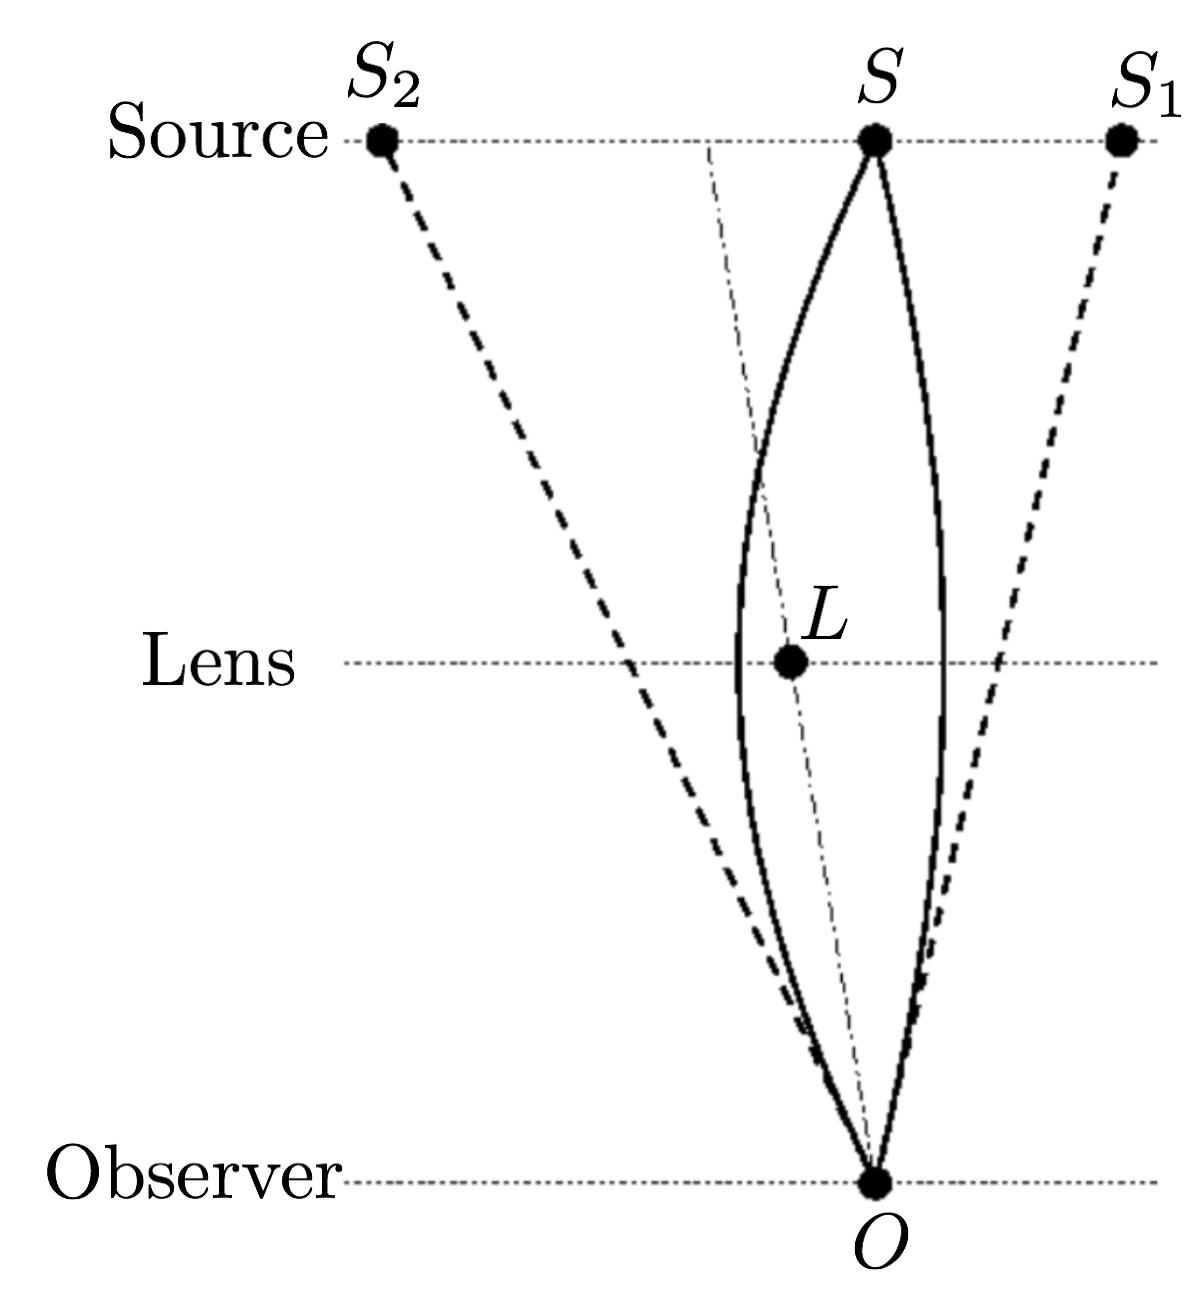
\includegraphics[width=7cm]{figures/GravitationalLens.png}
    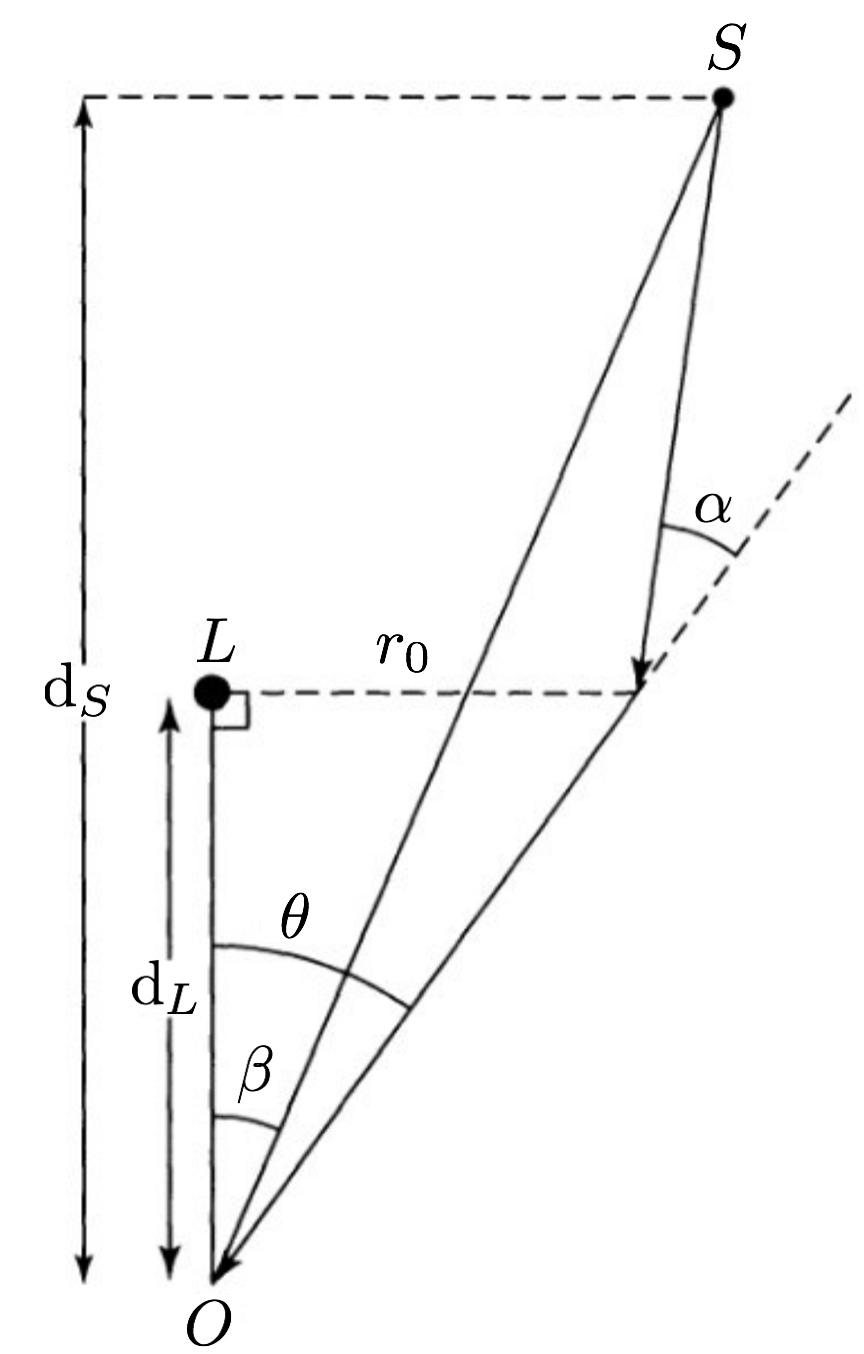
\includegraphics[width=5cm]{figures/GravitationalLensAngles.png}
    \caption{\footnotesize{\textbf{(Left)}: Setup of a gravitational lens. Figure taken from Abdo. \textbf{(Right)}: The geometry for a gravitational lens. The path of light is taken from a source at point $S$, as it is deflected through an angle $\alpha$, by the gravitational lens due to a point mass $M$ at point $L$. Figures adapted from Carroll \& Ostlie (2007).}}
    \label{fig:gravitationallens}
\end{figure}

{\noindent}The apparent speed of light, the rate at which the spatial coordinates of a photon change, is called the \textbf{coordinate speed of light}. Starting with the Schwarzschild metric with ${\rm d}s=0$,

\begin{align*}
    0 = \left(c{\rm d}t \sqrt{1-\frac{2GM}{rc^2}}\right)^2 - \left(\frac{{\rm d}r}{\sqrt{1-\frac{2GM}{rc^2}}}\right)^2 - (r{\rm d}\theta)^2 - (2\sin\theta{\rm d}\alpha)^2,
\end{align*}

{\noindent}we can calculate the coordinate speed of a vertically travelling photon. Inserting ${\rm d}\theta={\rm d}\alpha=0$ shows that, in general, the coordinate speed of light in the radial direction is

\begin{align*}
    \frac{{\rm d}r}{{\rm d}t} = c\left(1-\frac{2GM}{rc^2}\right) = c\left(1-\frac{r_S}{r}\right) ~ [{\rm m\,s^{-1}}],
\end{align*}

{\noindent}When $r\gg r_S$, ${\rm d}r/{\rm d}t\simeq c$, as expected in flat spacetime. However, at $r=r_S$, ${\rm d}r/{\rm d}t=0$.

{\noindent}Thus, the effective ``index of refraction'' is

\begin{align*}
    n = \frac{c}{{\rm d}r/{\rm d}t} = \left(1-\frac{2GM}{rc^2}\right)^{-1} \simeq 1+ \frac{2GM}{rc^2} ~ [{\rm dimensionless}]
\end{align*}

{\noindent}for radially travelling light, assuming that $r_S/r\ll1$. At a distance of $10^4\,{\rm pc}$ from a galaxy with a mass of $10^{11}\,{\rm M_\odot}$, the effective index of refraction is $n=1+9.6\times10^{-7}$. (Of course, the light passing by the point mass will never be travelling exactly radially. This was merely used to estimate the magnitude of the effect of gravity in a gravitational lens.) Obviously, the deviation of the light from a straight line will be extremely small. 

{\noindent}Figure \ref{fig:gravitationallens} shows the setup of a gravitational lens (left) as well as its detailed geometry (right). The path of light is taken from a source at point $S$, as it is deflected through an angle $\alpha$, by the gravitational lens due to a point mass $M$ at point $L$.

{\noindent}The angular deviation of a photon passing a distance $r_0$ (very nearly the distance of closest approach) from a mass $M$ is

\begin{align*}
    \alpha = \frac{4GM}{r_0c^2} ~ [{\rm rad}],
\end{align*}

{\noindent}which includes the factor of $2$ as a correction from the ``Newtonian'' value. The distance to the source is $d_S/\cos\beta\simeq d_S$ where $\beta\ll1$, and $d_L$ is the distance to the lensing mass. It is then a matter of simple trigonometry to show that the angle $\theta$ between between the lensing mass and the image of the source must satisfy the equation

\begin{align*}
    \theta^2 - \beta\theta - \frac{4GM}{c^2} \left(\frac{d_S-d_L}{d_Sd_L}\right) = 0
\end{align*}

{\noindent}where $\theta$ and $\beta$ are measured in radians.

{\noindent}This quadratic equation indicates that for the geometry shown in Figure \ref{fig:gravitationallens} (left) there will be two solutions for $\theta$, and so two images will be formed by the gravitational lens. Designating these solutions as $\theta_1$ and $\theta_2$, these angles can be measured observationally and then used to find the values of $\beta$ and $M$. The results are

\begin{align*}
    \beta = \theta_1 + \theta_2 ~ [{\rm rad}]
\end{align*}

{\noindent}and

\begin{align*}
    M = -\frac{\theta_1\theta_2c^2}{4G} \left(\frac{d_S-d_L}{d_Sd_L}\right) ~ [{\rm M_\odot}].
\end{align*}

{\noindent}Referring back to Figure \ref{fig:gravitationallens} (left) note that $\beta=\theta_1+\theta_2$ implies $\theta_1$ and $\theta_2$ have opposite signs. As a result, two images are formed on opposite sides of the gravitational lens, so $M$ will be positive.

% --------------------------------------------------------------
%               7. 
% --------------------------------------------------------------

\newpage
\subsection{Question 7}

What is the density-morphology relation for galaxies? How is that related to what we know about the relationship between galaxy density and star formation rates in galaxies?

\subsubsection{Short answer}

The density-morphology relation for galaxies is the relation between the density of galaxies and the likelihood of a particular galaxy morphology. In galaxy clusters, for example, elliptical galaxies are more commonly found in the high-density cluster centers whereas spirals are more commonly found at the lower density galaxy outskirts.

\subsubsection{Additional context}

The mixture of galaxy types in clusters seems to differ from that of isolated (field) galaxies. Whereas about 70\% of luminous field galaxies are spirals, clusters are dominated by early-type galaxies, in particular in their inner regions. Furthermore, the fraction of spirals in a cluster depends on the distance from the center and increases for larger $r$. Obviously, the local density has an effect on the morphological mix of galaxies. As in clusters, the fraction of group members which are spirals is lower than the fraction of spirals among field (i.e., isolated) galaxies, and the relative abundance of spiral galaxies decreases with increasing $\sigma_v$ of the group.

{\noindent}More generally, one may ask whether the mixture of the galaxy population depends on the local galaxy density. While earlier studies of this effect were frequently confined to galaxies within and around clusters, extensive redshift surveys like the 2dFGRS and the SDSS allow us to systematically investigate this question with very large and carefully selected samples of galaxies. The morphological classification of such large samples is performed by automated software tools, which basically measure the light concentration in the galaxies, or, alternatively, the best-fitting S\'ersic-index $n$. A comparison of galaxies classified this way with visual classifications shows very good agreement.

{\noindent}As an example of such an investigation, results from the Sloan Digital Sky Survey are shown in Figure \ref{fig:densitymorphology}. Galaxies were morphologically classified, based on SDSS photometry, and separated into four classes, corresponding to elliptical galaxies, S0 galaxies, and early (Sa) and late (Sc) types of spiral. In this analysis, only galaxies were included for which the redshift was spectroscopically measured. Therefore, the spatial galaxy density can be estimated. However, one needs to take into account the fact that the measured redshift is a superposition of the cosmic expansion and the peculiar velocity of a galaxy. The peculiar velocity may have rather large values ($1,000\,{\rm km\,s^{-1}}$), in particular in clusters of galaxies. For this reason, for each galaxy in the sample the surface number density of galaxies which have a redshift within $1,000\,{\rm km\,s^{-1}}$ of the target galaxy was determined. The left panel in Figure \ref{fig:densitymorphology} shows the fraction of the different galaxy classes as a function of this local galaxy density. A very clear dependence, in particular of the fraction of late-type spirals, on the local density can be seen: in regions of higher galaxy density Sc-spirals contribute less than 10\% of the galaxies, whereas their fraction is about 30\% in low-density regions. Combined, the fraction of spirals decreases from 65\% in the field to about 35\% in regions of high galaxy density. In contrast, the fraction of ellipticals and S0 galaxies increases towards higher densities, with the increase being strongest for ellipticals.

\begin{figure}[t!]
    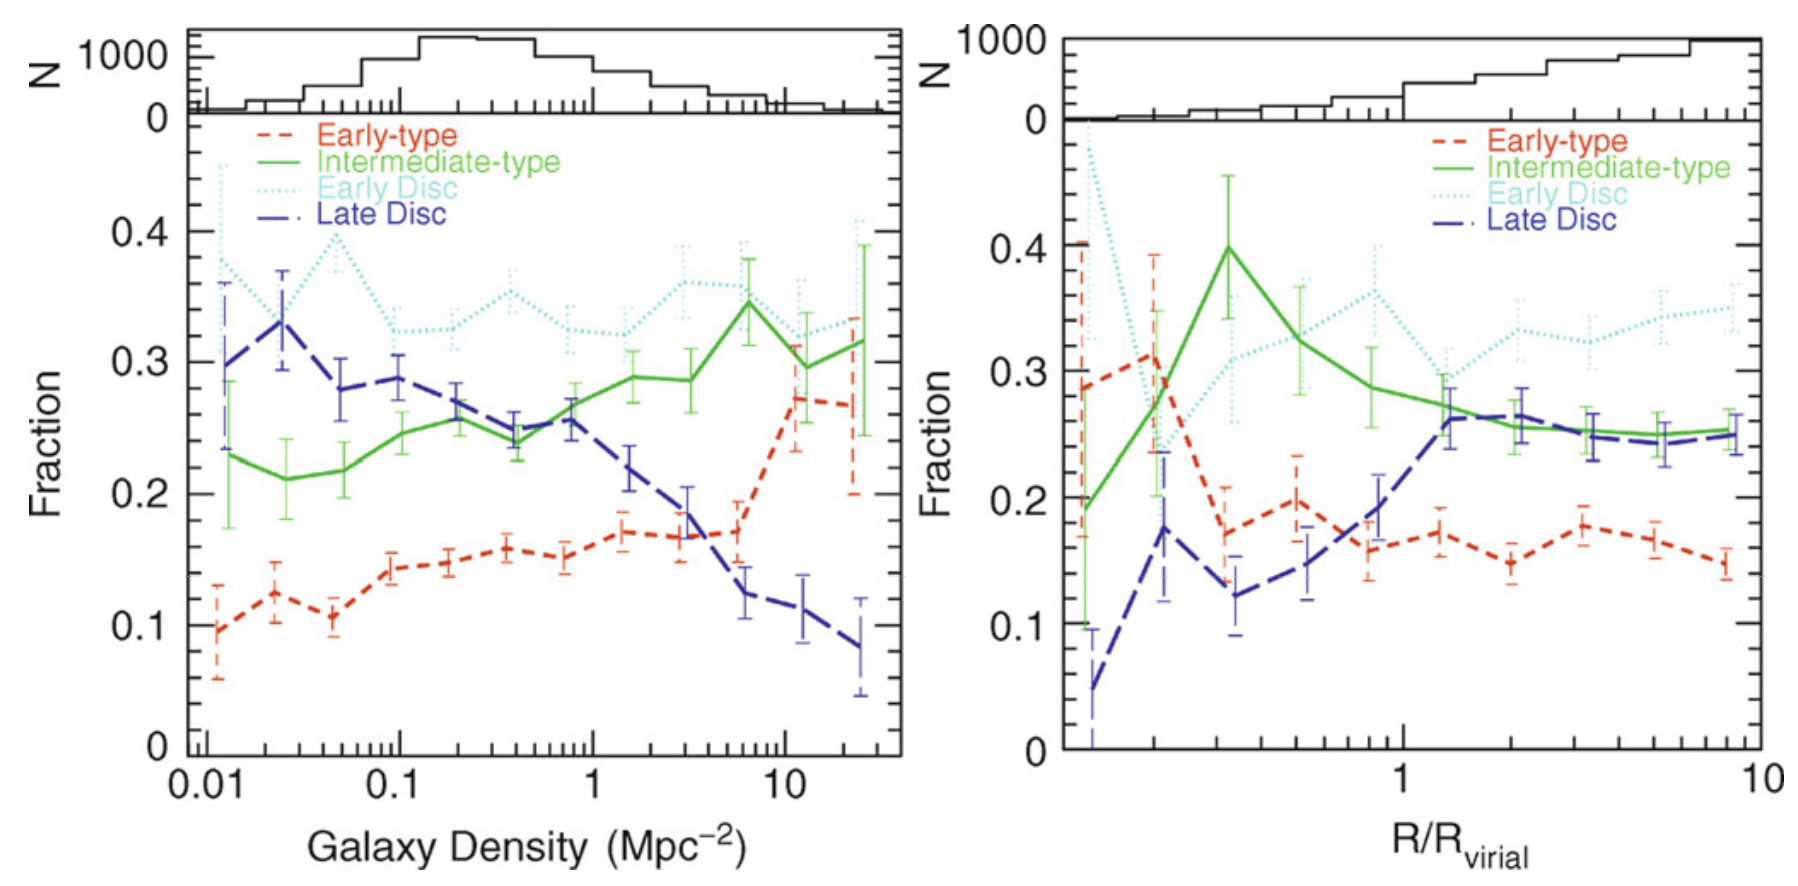
\includegraphics[width=16cm]{figures/DensityMorphology.png}
    \centering
    \caption{\footnotesize{The number fraction of galaxies of different morphologies is plotted as a function of the local galaxy density (left panel), and for galaxies in clusters as a function of the distance from the cluster center, scaled by the corresponding virial radius (right panel). Galaxies are divided into four different classes. `Early-types' contain mainly ellipticals, `intermediates' are mainly S0 galaxies, `early and late discs' are predominantly Sa and Sc spirals, respectively. In both representations, a clear dependence of the galaxy mix on the density or on the distance from the cluster center, respectively, is visible. In the histograms at the top of each panel, the number of galaxies in the various bins is plotted. Source: T. Goto et al. 2003, The morphology-density relation in the Sloan Digital Sky Survey, MNRAS 346, 601, p. 607, 608, Figs. 12, 15. Figure taken from Schneider (2006).}}
    \label{fig:densitymorphology}
\end{figure}

{\noindent}In the right-hand panel of Figure \ref{fig:densitymorphology}, the mixture of galaxy morphologies is plotted as a function of the distance to the center of the nearest cluster, where the distance is scaled by the virial radius of the corresponding cluster. As expected, a very strong dependence of the fraction of ellipticals and spirals on this distance is seen. Sc spirals contribute a mere 5\% of galaxies in the vicinity of cluster centers, whereas the fraction of ellipticals and S0-galaxies strongly increases inwards.

{\noindent}The two diagrams in Figure \ref{fig:densitymorphology} are of course not mutually independent: a region of high galaxy density is very likely to be located in the vicinity of a cluster center, and the opposite is valid accordingly. Therefore, it is not immediately clear whether the mix of galaxy morphologies depends primarily on the respective density of the environment of the galaxies, or whether it is caused by morphological transformations in the inner regions of galaxy clusters.

{\noindent}The density-morphology relation is also seen in galaxy groups. The fraction of late-type galaxies decreases, and the fraction of early-type galaxies increases with decreasing distance from the group center, as is also the case in clusters. When considering the morphological mix of visually classified early- and late-type galaxies, averaged over the whole group or cluster (i.e., up to the virial radius) then it seems to be constant for group/cluster halo masses in excess of $\sim10^{13}\,{\rm M_\odot}$.

{\noindent}A closer examination of Figure \ref{fig:densitymorphology} may provide a clue as to what physical processes are responsible for the dependence of the morphological mix on the local number density. We consider first the right-hand panel of Figure \ref{fig:densitymorphology}. Three different regimes in radius can be identified: for $R\gtrsim R_\mathrm{vir}$, the fraction of the different galaxy types remains basically constant. In the intermediate regime, $0.3\lesssim R/R_\mathrm{vir}\lesssim1$, the fraction of S0 galaxies strongly increases inwards, whereas the fraction of late-type spirals decreases accordingly. This result is compatible with the interpretation that in the outer regions of galaxy clusters spirals lose gas, for instance by their motion through the intergalactic medium (IGM), and these galaxies then transform into passive S0 galaxies. Below $R\lesssim0.3\,R_\mathrm{vir}$, the fraction of S0 galaxies decreases strongly, and the fraction of ellipticals increases substantially.

{\noindent}In fact, the ratio of the number densities of S0 galaxies and ellipticals, for $R\lesssim0.3\,R_\mathrm{vir}$, strongly decreases as $R$ decreases. This may hint at a morphological transformation in which S0 galaxies are turned into ellipticals, probably by collisions or mergers. Such gas-free mergers, also called `dry mergers', may be the preferred explanation for the generation of elliptical galaxies. One of the essential properties of dry mergers is that such a merging process would not be accompanied by a burst of star formation, unlike the case of gas-rich collisions of galaxies. The existence of a population of newly born stars in ellipticals would be difficult to reconcile with the generally old stellar population actually observed in these galaxies.

{\noindent}Considering now the dependence on local galaxy density (the left-hand panel of Figure \ref{fig:densitymorphology}), a similar behavior of the morphological mix of galaxies is observed: there seems to exist two characteristic values for the galaxy density where the relative fractions of galaxy morphologies change noticeably. Interestingly, the relation between morphology and density seems to evolve only marginally between $z=0.5$ and the local Universe.

{\noindent}One clue as to the origin of the morphological transformation of galaxies in clusters, as a function of distance from the cluster center, comes from the observation that the velocity dispersion of very bright cluster galaxies seems to be significantly smaller than that of less luminous ones. Assuming that the mass-to-light ratio does not vary substantially among cluster members, this then indicates that the most massive galaxies have smaller velocity dispersions. One way to achieve this trend in the course of cluster evolution is by dynamical interactions between cluster galaxies. Such interactions tend to `thermalize' the velocity distribution of galaxies, so that the mean kinetic energy of galaxies tends to become similar. This then causes more massive galaxies to become slower on average. If this interpretation holds, then the morphology-density relation may be attributed to these dynamical interactions, rather than to the (so-called ram-pressure) stripping of the ISM as the galaxies move through the ICM. However, ram-pressure stripping of the ISM has been clearly observed in clusters. This effect mostly acts on the atomic gas of spirals, whereas the molecular gas seems to be less affected; we recall that the molecular gas is more densely concentrated towards the galactic disk, and thus more strongly bound. In fact, it has been known for a long time that there are spiral galaxies in groups and clusters which are deficient in neutral hydrogen, relative to field galaxies of the same stellar luminosity. If ram-pressure stripping, or other effects in the dense cluster environment, removes the ISM from spirals, then the result could be a disk galaxy without ongoing star formation -- something that may resemble an S0 galaxy. If that were the case, than S0s would be passively fading former spirals. Whereas the original spirals satisfied the Tully-Fisher relation, the S0s would then be expected to be considerably fainter than spirals, at fixed rotational velocity; this indeed is the case.

\subsubsection{Follow-up Questions}

\begin{itemize}
    \item What processes in a cluster convert galaxies?
    \item Where is galaxy harassment most effective (due to relative speeds)?
\end{itemize}


% --------------------------------------------------------------
%               8. 
% --------------------------------------------------------------

\newpage
\subsection{Question 8}

Draw the spectral energy distribution (SED) of a galaxy formed by a single burst of star formation at the ages of $10\,\mathrm{Myrs}$, $2\,\mathrm{Gyrs}$, and $10\,\mathrm{Gyr}$. Please highlight the change over time in the $4000$ Angstrom break.

\subsubsection{Short answer}

\begin{figure}[h]
    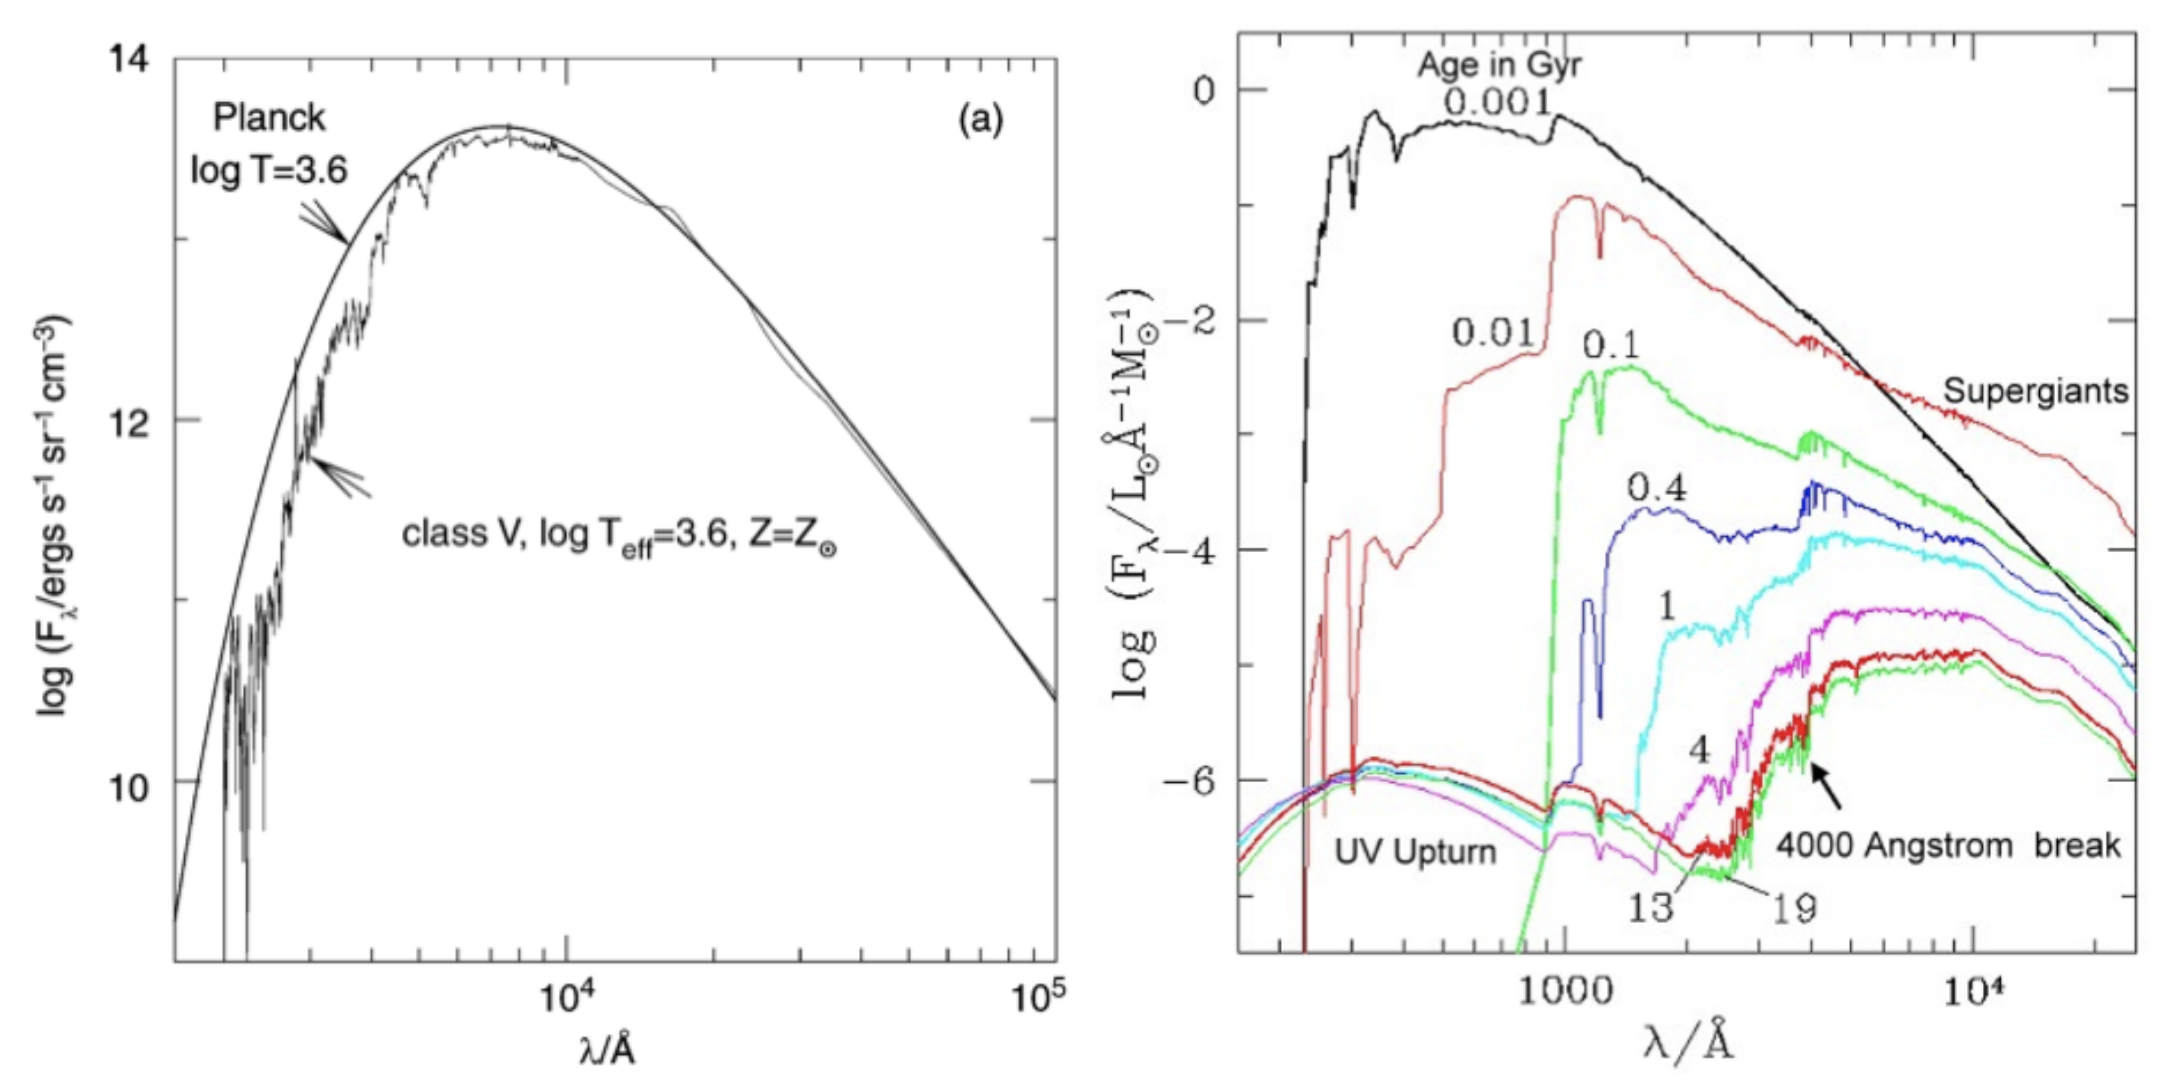
\includegraphics[width=16cm]{figures/SED_SF.png}
    \centering
    \caption{\footnotesize{(a) Comparison of the spectrum of a MS star with a black body spectrum of equal effective temperature. The opacity of the stellar atmosphere causes clear deviations from the Planck spectrum in the UV/optical. (b) Spectrum of a stellar population with Solar metallicity that was instantaneously born a time $t$ ago; t is given in units of $10^9\,{\rm yr}$. Source: S. Charlot 1996, Spectral Evolution of Galaxies, Lecture Notes in Physics 470, Springer-Verlag, p. 53. Figure taken from Schneider (2006).}}
    \label{fig:sedsf}
\end{figure}

\subsubsection{Additional context}

{\noindent}The light of normal galaxies originates from stars. Stellar evolution is largely understood, and the spectral radiation of stars can be calculated from the theory of stellar atmospheres. If the distribution of the number density of stars is known as a function of their mass, chemical composition, and evolutionary stage, we can compute the light emitted by them. The theory of population synthesis aims at interpreting the spectrum of galaxies as a superposition of stellar spectra. We have to take into account the fact that the distribution of stars changes over time; e.g., massive stars leave the main sequence after several $10^6\,{\rm yr}$, the number of luminous blue stars thus decreases, which means that the spectral distribution of the population also changes in time. The spectral energy distribution (SED) of a galaxy thus reflects its history of star formation (SF) and stellar evolution. For this reason, simulating different SF histories and comparing them with observed galaxy spectra provides important clues for understanding the evolution of galaxies. Let's discuss some aspects of the theory of population synthesis; this subject is of tremendous importance for our understanding of galaxy spectra.

{\noindent}The processes of SF are not understood in detail; for instance, it is currently impossible to compute the mass spectrum of a group of stars that jointly formed in a molecular cloud. Obviously, high-mass and low-mass stars are born together and form young (open) star clusters. The mass spectra of these stars are determined empirically from observations.

{\noindent}The initial mass function (IMF) is defined as the initial mass distribution at the time of birth of the stars, such that $\xi(m)\mathrm{d}m$ specifies the fraction of stars in the mass interval of width $\mathrm{d}m$ around $m$, where the distribution is normalized,

\begin{align*}
    \int\limits_{m_L}^{m_U} m\xi(m)\,\mathrm{d}m = 1\,{\rm M}_\odot.
\end{align*}

{\noindent}The integration limits are not well defined. Typically, one uses $m_L=0.1\,{\rm M_\odot}$ because stars less massive than $\approx0.08\,{\rm M_\odot}$ do not ignite their hydrogen (and are thus brown dwarfs), and $m_U\sim100\,{\rm M_\odot}$ because considerably more massive stars are not observed. Whereas such very massive stars would in any case be difficult to observe because of their very short lifetime, the theory of stellar structure tells us that more massive stars can probably not form a stable configuration due to excessive radiation pressure. The shape of the IMF is also subject to uncertainties; in most cases, the Salpeter-IMF is used,

\begin{align*}
    \xi(m) \propto m^{-2.35} ~ [{\rm dimensionless}],
\end{align*}

{\noindent}as obtained from investigating the stellar mass spectrum in young star clusters. It is by no means clear whether a universal IMF exists, or whether it depends on specific conditions like metallicity, the mass of the galaxy, cosmic epoch, or other parameters. Given the difficulties of determining the shape of the IMF, apparent variations of the IMF with epoch or environment may be attributed to other effect, such as the specifics of the star-formation history in galaxies. Therefore, there seems to be no clear direct indication that the IMF varies with environment. However, some properties of high-redshift galaxies are very difficult to understand if their IMF was the same as in our neighborhood. It has therefore been suggested that the IMF in starbursts is different from that of quiescent star formation such as we are experiencing in the Milky Way.

{\noindent}The Salpeter-IMF seems to be a good description for stars with $M\gtrsim1\,{\rm M_\odot}$, whereas the IMF for less massive stars is flatter. Note that, due to the steep slope of the IMF, most of the stellar mass is contained in low-mass stars. However, since the luminosity of main-sequence stars depends strongly on mass, approximately as $L\propto M^3$, most of the luminosity comes from high-mass stars.

{\noindent}The star-formation rate (SFR) is the gas mass that is converted into stars per unit time,

\begin{align*}
    \mathrm{SFR} = -\frac{\mathrm{d}M_\mathrm{gas}}{\mathrm{d}t} ~ [{\rm M_\odot\,yr^{-1}}].
\end{align*}

{\noindent}The metallicity $Z$ of the ISM defines the metallicity of the newborn stars, and the stellar properties in turn depend on $Z$. During stellar evolution, metal-enriched matter is ejected into the ISM by stellar winds, planetary nebulae, and SNe, so that $Z(t)$ is an increasing function of time. This chemical enrichment must be taken into account in population synthesis studies in a self-consistent form.

\begin{figure}[t]
    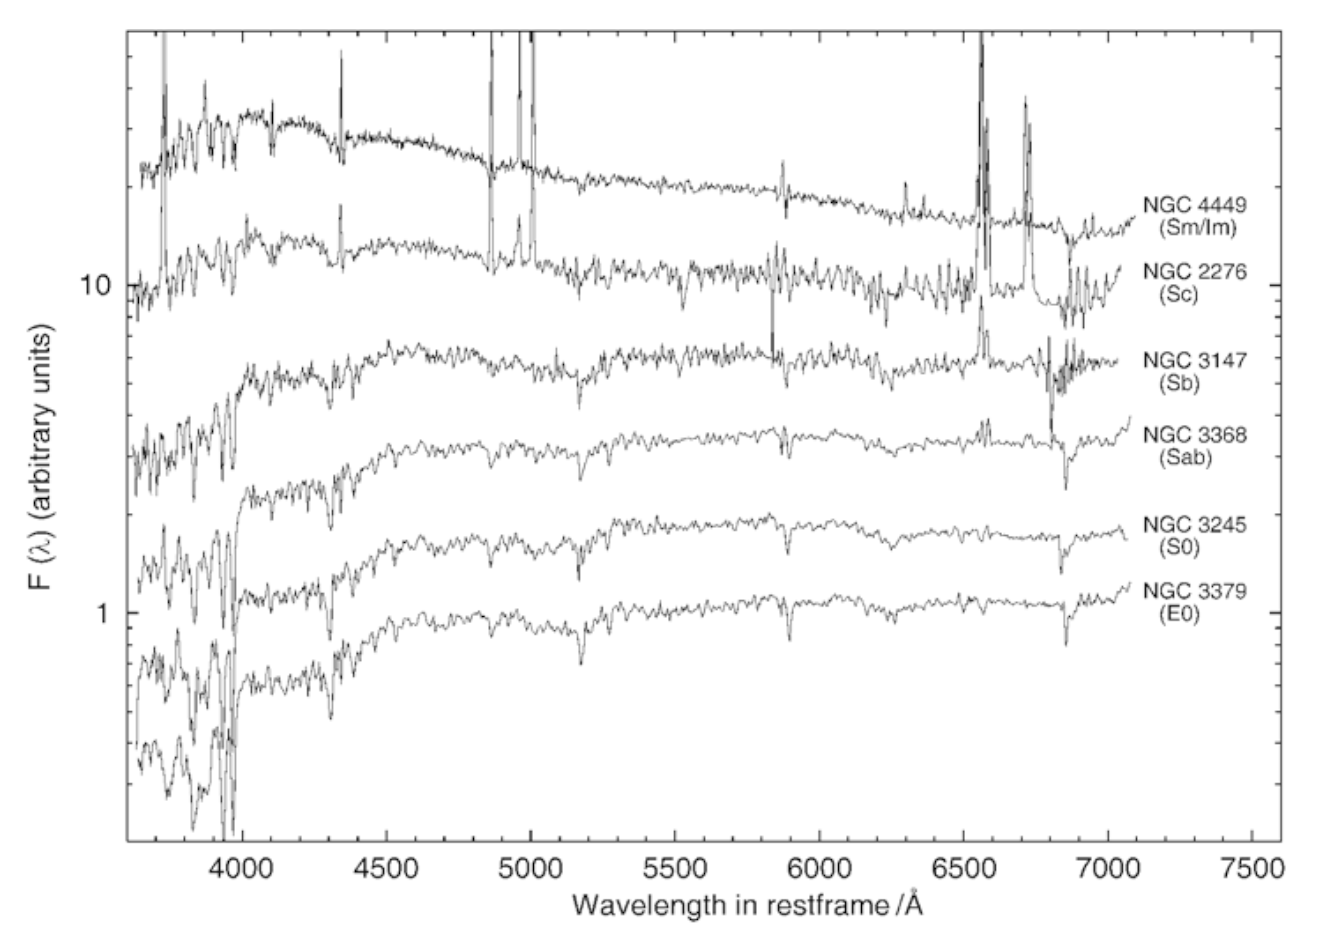
\includegraphics[width=16cm]{figures/StellarSpectra.png}
    \centering
    \caption{\footnotesize{Spectra of galaxies of different types, where the spectral flux is plotted logarithmically in arbitrary units. The spectra are ordered according to the Hubble sequence, with early types at the bottom and late-type spectra at the top. Data from R. Kennicutt 1992, ApJS 79, 255. Figure taken from Schneider (2006).}}
    \label{fig:stellarspectra}
\end{figure}

{\noindent}Let $S_{\lambda,Z}(t')$ be the emitted energy per wavelength and time interval, normalized to an initial total mass of $1\,{\rm M_\odot}$, emitted by a group of stars of initial metallicity $Z$ and age $t_0$. The function $S_{\lambda,Z(t-t_0)}(t')$, which describes this emission at any point $t$ in time, accounts for the different evolutionary tracks of the stars in the (HRD). It also accounts for their initial metallicity (i.e., at time $t-t'$), where the latter follows from the chemical evolution of the ISM of the corresponding galaxy. Then the total spectral luminosity of this galaxy at a time $t$ is given by

\begin{align*}
    F_\lambda(t) = \int\limits_0^t \mathrm{SFR}(t-t')S_{\lambda,Z(t-t')}(t')\,\mathrm{d}t' ~ [{\rm erg\,s^{-1}\,cm^{-2}\,Hz^{-1}}],
\end{align*}

{\noindent}thus by the convolution of the star formation rate with the spectral energy distribution of the stellar population. In particular, $F_\lambda(t)$ depends on the star formation history.

{\noindent}In the beginning, the spectrum and luminosity of a stellar population are dominated by the most massive stars, which emit intense UV radiation. But after $\sim10^7\,{\rm yr}$, the flux below $1,000$\,\AA\,is diminished significantly, and after $\sim10^8\,{\rm yr}$, it hardly exists any more. At the same time, the flux in the NIR increases because the massive stars evolve into red supergiants.

{\noindent}For $10^8\,{\rm yr}\gtrsim t\gtrsim10^9\,{\rm yr}$, the emission in the NIR remains high, whereas short-wavelength radiation is more and more diminished. After $\sim10^9\,{\rm yr}$, red giant stars (RGB stars) account for most of the NIR production. After $\sim3\times10^9\,{\rm yr}$, the UV radiation increases again slightly, due to blue stars on the horizontal branch into which stars evolve after the AGB phase, and due to white dwarfs which are hot when they are born. Between an age of $4$ and $13$ billion years, the spectrum of a stellar population evolves fairly little. 

{\noindent}Of particular importance is the spectral break located at about $4,000$\,\AA~(see Figure \ref{fig:sedsf}) which becomes visible in the spectrum after a few $10^7\,{\rm yr}$. This break is caused by a strongly changing opacity of stellar atmospheres at this wavelength, mainly due to strong transitions of singly ionized calcium and the Balmer lines of hydrogen. Hence, the radiation from a stellar population at $<4,000$\,\AA~is less intense than at $>4,000$\,\AA; this is the case particularly for early-type galaxies, as can be seen in Figure \ref{fig:stellarspectra}, due to their old stellar population. This $4,000$\,\AA break is one of the most important spectral properties of the continuum stellar emission in galaxies; it allows us to estimate the redshifts of early-type galaxies from their photometric properties -- so-called photometric redshift estimates.

\subsubsection{Follow-up Questions}

\begin{itemize}
    \item Why do we only consider a single burst of SF? (Want to hear about population synthesis.)
    \item If you looked at an actual SED, what else would you see besides the mostly smooth continuum and spectral breaks?
    \item What's a typical emission line you would see in the optical part of the spectrum?
    \item Why is the y-axis is $\lambda\mathrm{F}_\lambda$, what does that mean?
\end{itemize}


% --------------------------------------------------------------
%               9. 
% --------------------------------------------------------------

\newpage
\subsection{Question 9}

How are galaxy redshifts estimated by photometric techniques?

\subsubsection{Short answer}

Well-defined spectral features are typically used for photometric redshift measurements since the location of these breaks in wavelength depends directly on the redshift. The most common breaks include the $4000$\,\AA~break (from ionized metals in stellar photospheres) and the $1216$\,\AA~Lyman break (from neutral hydrogen in the IGM along the line-of-sight).

\subsubsection{Additional context}

The Lyman-break technique is a special case of a method for estimating the redshift of galaxies (and QSOs) by multi-color photometry. This technique can be employed due to the spectral breaks at $912\,$\AA and $1216\,$\AA, respectively. Spectra of galaxies also show other characteristic features. The broadband energy distribution is basically a superposition of stellar radiation (if we ignore for a moment the presence of dust, which can yield a substantial infrared emission from galaxies). A stellar population of age $\gtrsim10^8\,{\rm yr}$ features a $4,000$\,\AA~break because, due to a sudden change in the opacity at this wavelength, the spectra of most stars show such a break at about $4,000$\,\AA~(see Figure \ref{fig:sedsf}). Hence, the radiation from a stellar population at $<4,000$\,\AA~is less intense than at $>4,000$\,\AA; this is the case particularly for early-type galaxies, as can be seen in Figure \ref{fig:stellarspectra}, due to their old stellar population.

{\noindent}If we assume that the star-formation histories of galaxies are not too diversified, the spectral energy distributions of these galaxies are expected to follow certain patterns. For example, if all galaxies had a single episode of star formation, starting at their formation redshift $z_f$ and lasting for a time $t$, then the spectra of these galaxies, for a given initial mass function, would be characterized by these two parameters, as well as the total stellar mass formed; this latter quantity then yields the amplitude of the spectrum, but does not affect the spectral shape. When measuring the magnitude of these galaxies in $n$ broad-band filters, we can form $n-1$ independent colors. Next suppose we form a multidimensional CCD, in which every galaxy is represented by a point in this ($n-1$)-dimensional color space. Considering only galaxies at the present epoch, all these points will lie on a two-dimensional surface in this multi-dimensional space, instead of being more or less randomly distributed.

{\noindent}Next, instead of plotting $z=0$ galaxies, we consider the distribution of galaxies at some higher redshift $z<z_f$. This distribution of points will be different, mainly due to two different effects. First, a given photometric filter corresponds to a different rest-frame spectral range of the galaxy, due to redshift. Second, the ages of the stellar populations are younger at an earlier cosmic epoch, and thus the spectral energy distributions are different. Both of these effects will cause these redshift $z$ galaxies to occupy a different two-dimensional surface in multi-color space.

{\noindent}Generalizing this argument further, we see that in this idealized consideration, galaxies will occupy a three-dimensional subspace in ($n-1$)-dimensional color space, parametrized by formation redshift $z_f$, time-scale $t$, and the galaxy’s redshift $z$. Hence, from the measurement of the broad-band energy distribution of a galaxy, we might expect to be able to determine, or at least estimate, its redshift, as well as other properties such as the age of its stellar population; this is the principle of the method of photometric redshifts.

\begin{figure}[h]
    \floatbox[{\capbeside\thisfloatsetup{capbesideposition={right,top},capbesidewidth=4cm}}]{figure}[\FBwidth]
    {\caption{\footnotesize{The bottom panel illustrates again the principle of the drop-out method, for a galaxy at $z\sim3.2$. Whereas the Lyman-$\alpha$ forest absorbs part of the spectral flux between (rest-frame wavelength) $912$ and $1216$\,\AA, the flux below $912$\,\AA~vanishes almost completely. By using different combinations of filters (top panel), an efficient selection of galaxies at other redshifts is also possible. The example shows a galaxy at $z=1$ whose $4,000$\,\AA~break is located between the two redder filters. The $4,000$\,\AA~break occurs in stellar populations after several $10^7\,{\rm yr}$ (see Figure \ref{fig:sedsf}) and is one of the most important features for the method of photometric redshift. Source: K.L. Adelberger 1999, Star Formation and Structure Formation at Redshifts $1<z<4$, astro-ph/9912153, Fig. 1. Figure taken from Schneider (2006).}}
    \label{fig:photredshifts}}
    {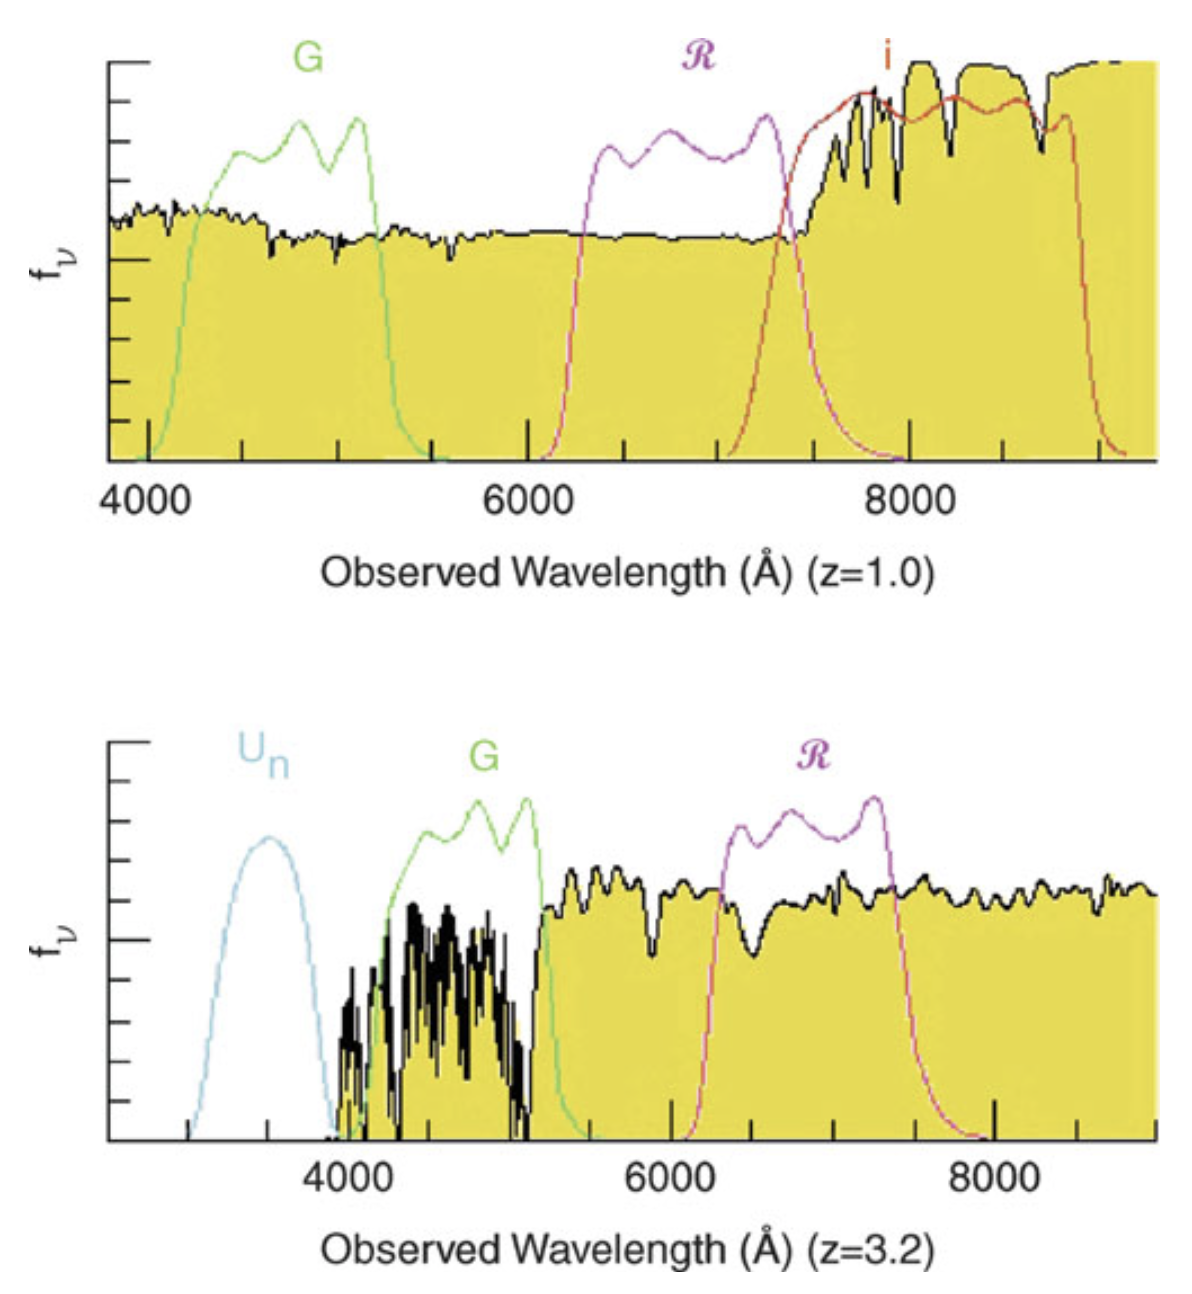
\includegraphics[width=11cm]{figures/PhotRedshifts.png}}
\end{figure}

{\noindent}Of course, the situation is considerably more complicated in reality. Galaxies most likely have a more complicated SF history than assumed here, and hence they will not be confined to a two-dimensional surface at fixed redshift, but instead will be spread around this surface. The spectrum of a stellar population also depends on its metallicity, as well as absorption, either by gas and dust in the ISM or hydrogen in intergalactic space (of which the Lyman-break method makes proper use). On the other hand, the colors of current-day galaxies are remarkably similar, best indicated by the red sequence. Therefore, the method of photometric redshifts may be expected to work, even if more complications are accounted for than in the idealized example considered above.

{\noindent}The method is strongly aided if the galaxies have characteristic spectral features, which shift in wavelength as the redshift is changed. If, for example, the spectrum of a galaxy was a power law in wavelength, then the redshifted spectrum would as well be a power law, with the same spectral slope -- if we ignore the different age of the stellar population. Therefore, for such an SED is would be impossible to estimate a redshift. However, if the spectrum shows a clear spectral break, then the location of this break in wavelength depends directly on the redshift, thus yielding a particularly clean diagnostic. In this context the $4,000$\,\AA~break and the Ly$\alpha$-break play a central role, as is illustrated in Figure \ref{fig:photredshifts}.

{\noindent}In order to apply this method, one needs to find the characteristic domains in color space where (most of) the galaxies are situated. This can be done either empirically, using observed SEDs of galaxies, or by employing population synthesis models. More precisely, a number of standard spectra of galaxies (so-called templates) are used, which are either selected from observed galaxies or computed by population synthesis models. Each of these template spectra can then be redshifted in wavelength. For each template spectrum and any redshift, the expected galaxy colors are determined by integrating the spectral energy distribution, multiplied by the transmission functions of the applied filters, over wavelength. This set of colors can then be compared with the observed colors of galaxies, and the set best resembling the observation is taken as an estimate for not only the redshift but also the galaxy type.

{\noindent}The advantage of this method is that multi-color photometry is much less time-consuming than spectroscopy of galaxies. Whereas some modern spectrographs allow one to take spectra of $\sim1,000$ objects simultaneously, images taken with wide-field cameras of $1\,\mathrm{deg}^2$ on $4\,{\rm m}$ class telescopes record the fluxes of $10^5$ galaxies in a one hour exposure. In addition, this method can be extended to much fainter magnitudes than are achievable for spectroscopic redshifts. The disadvantage of the method becomes obvious when an insufficient number of photometric bands are available, since then the photometric redshift estimates can yield a completely wrong $z$; these are often called catastrophic outliers. One example for the occurrence of extremely wrong redshift estimates is provided by a break in the spectral energy distribution. Depending of whether this break is identified as the Lyman-break or the $4,000$\,\AA~break, the resulting redshift estimates will be very different. To break the corresponding degeneracy, a sufficiently large number of filters spread over a broad spectral range must be available to probe the spectral energy distribution over a wide range in wavelengths. As a general rule, the more photometric bands are available and the smaller the uncertainties in the measured magnitudes, the more accurate the estimated redshift. Normally, data from four or five photometric bands are required to obtain useful redshift estimates. In particular, the reliability of the photometric redshift benefits from data over a large wavelength range, so that a combination of several optical and NIR filters is desirable.

{\noindent}The successful application of this method also depends on the type of the galaxies. Early-type galaxies form a relatively well-defined color-magnitude sequence at any redshift, due to their old stellar populations (manifested in clusters of galaxies in form of the red cluster sequence), so that the redshift of this type of galaxy can be estimated very accurately from multi-color information. However, this is only the case if the $4,000$\,\AA~break is located in between two of the applied filters. For $z\sim1$ this is no longer the case if only optical filters are used. Other types of galaxies show larger variations in their spectral energy distribution, depending, e.g., on the star formation history, as mentioned before.

{\noindent}Photometric redshifts are particularly useful for statistical purposes, for instance in situations in which the exact redshift of each individual galaxy in a sample is of little relevance. However, by using a sufficient number of optical and NIR filters, quite accurate redshift estimates for individual galaxies are achievable. For example, with eight optical and NIR bands and accurate photometry, a redshift accuracy of  $\Delta z\sim0.03(1+z)$ was obtained, as demonstrated in Figure \ref{fig:photvsspecredshift} by a comparison of photometric redshifts with redshifts determined spectroscopically for galaxies in the field of the HDF-North. If data in additional photometric bands are available, e.g., using filters of smaller transmission curves (`intermediate width filters'), the redshift accuracy can be increased even more, e.g., $\Delta z\sim0.01(1+z)$ was obtained using a total of 30 photometric bands.

\begin{figure}[t]
    \floatbox[{\capbeside\thisfloatsetup{capbesideposition={right,top},capbesidewidth=4cm}}]{figure}[\FBwidth]
    {\caption{\footnotesize{Photometric redshift versus the spectroscopic redshift for galaxies in the HDF-North. Photometric data in four optical and two NIR bands have been used here. We see how accurate photometric redshifts can be -- their quality depends on the photometric accuracy in the individual filters, the number of filters used, the redshift and the type of the galaxy, and also on details of the applied analysis method. Source: N. Benítez 2000, Bayesian Photometric Redshift Estimation, ApJ 536, 571, p. 579, Fig. 5. Figure taken from Schneider (2006).}}
    \label{fig:photvsspecredshift}}
    {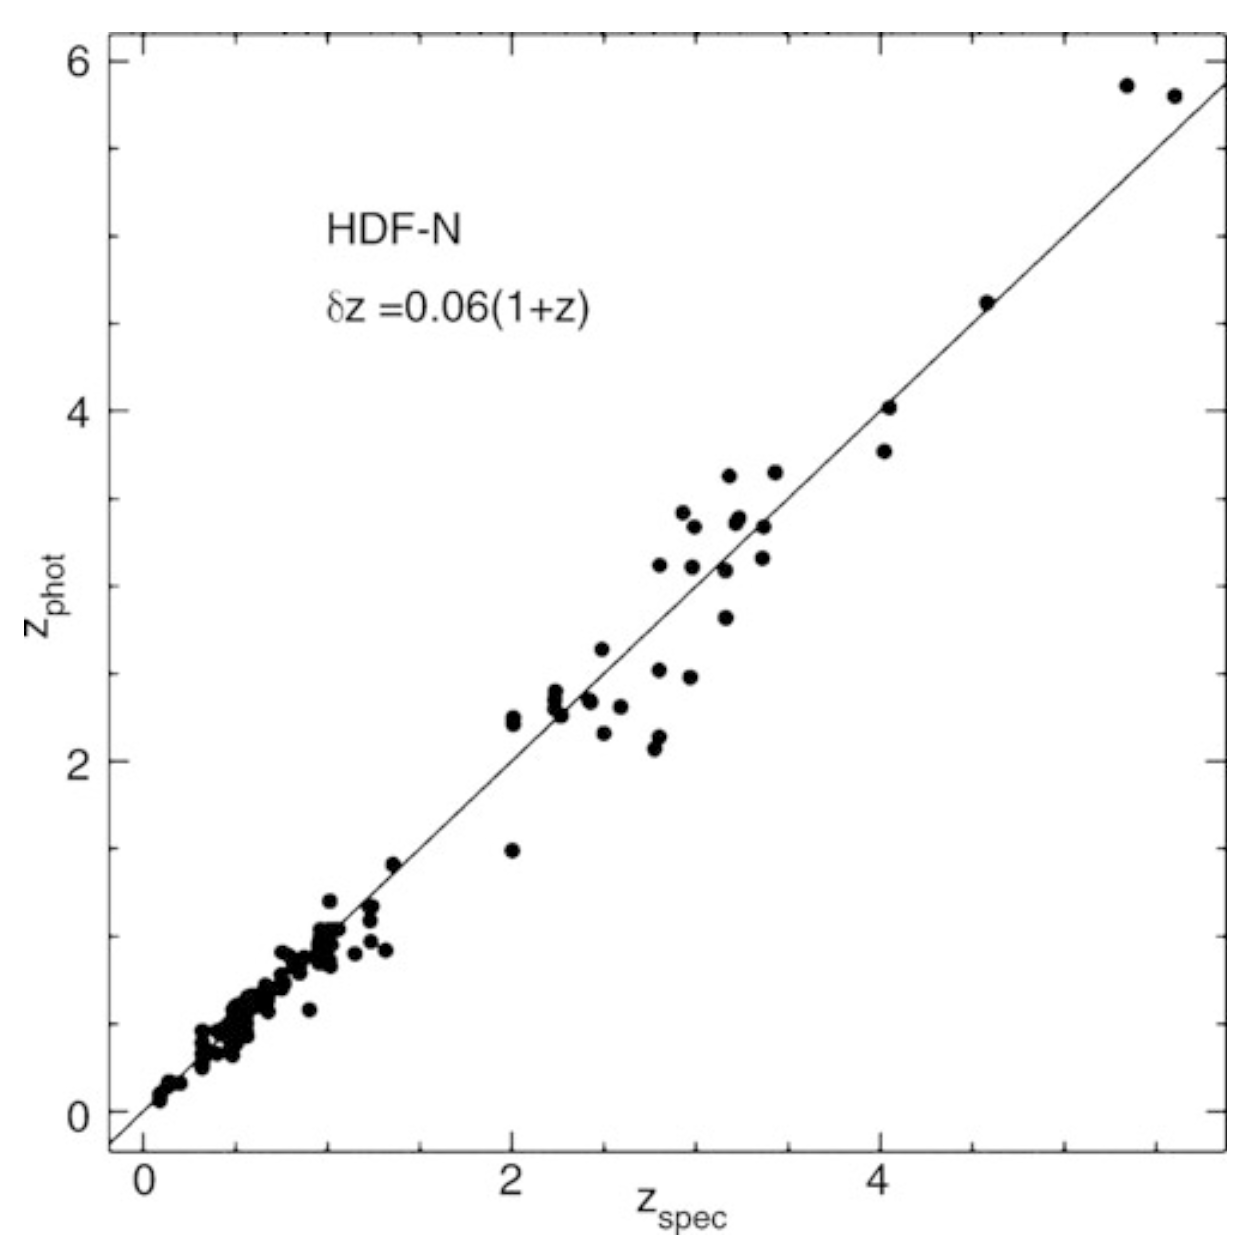
\includegraphics[width=8cm]{figures/PhotVsSpecRedshift.png}}
\end{figure}

\subsubsection{Follow-up Questions}

\begin{itemize}
    \item What problems are there with the photometric method?
    \item How do you account for different galaxy types, and what do you need to know about the stellar population? (i.e., IMF.)
    \item Can you use the $1216$\,\AA~break at high redshifts? (Wanted to hear about ionization.)
\end{itemize}


% --------------------------------------------------------------
%               10. 
% --------------------------------------------------------------

\newpage
\subsection{Question 10}

Draw a spectrum of a high-redshift quasar. What do quasar emission lines typically look like? Explain what we see in the spectrum at rest wavelengths bluer than $1216$ Angstroms.

\subsubsection{Short answer}

\begin{figure}[h]
    \centering
    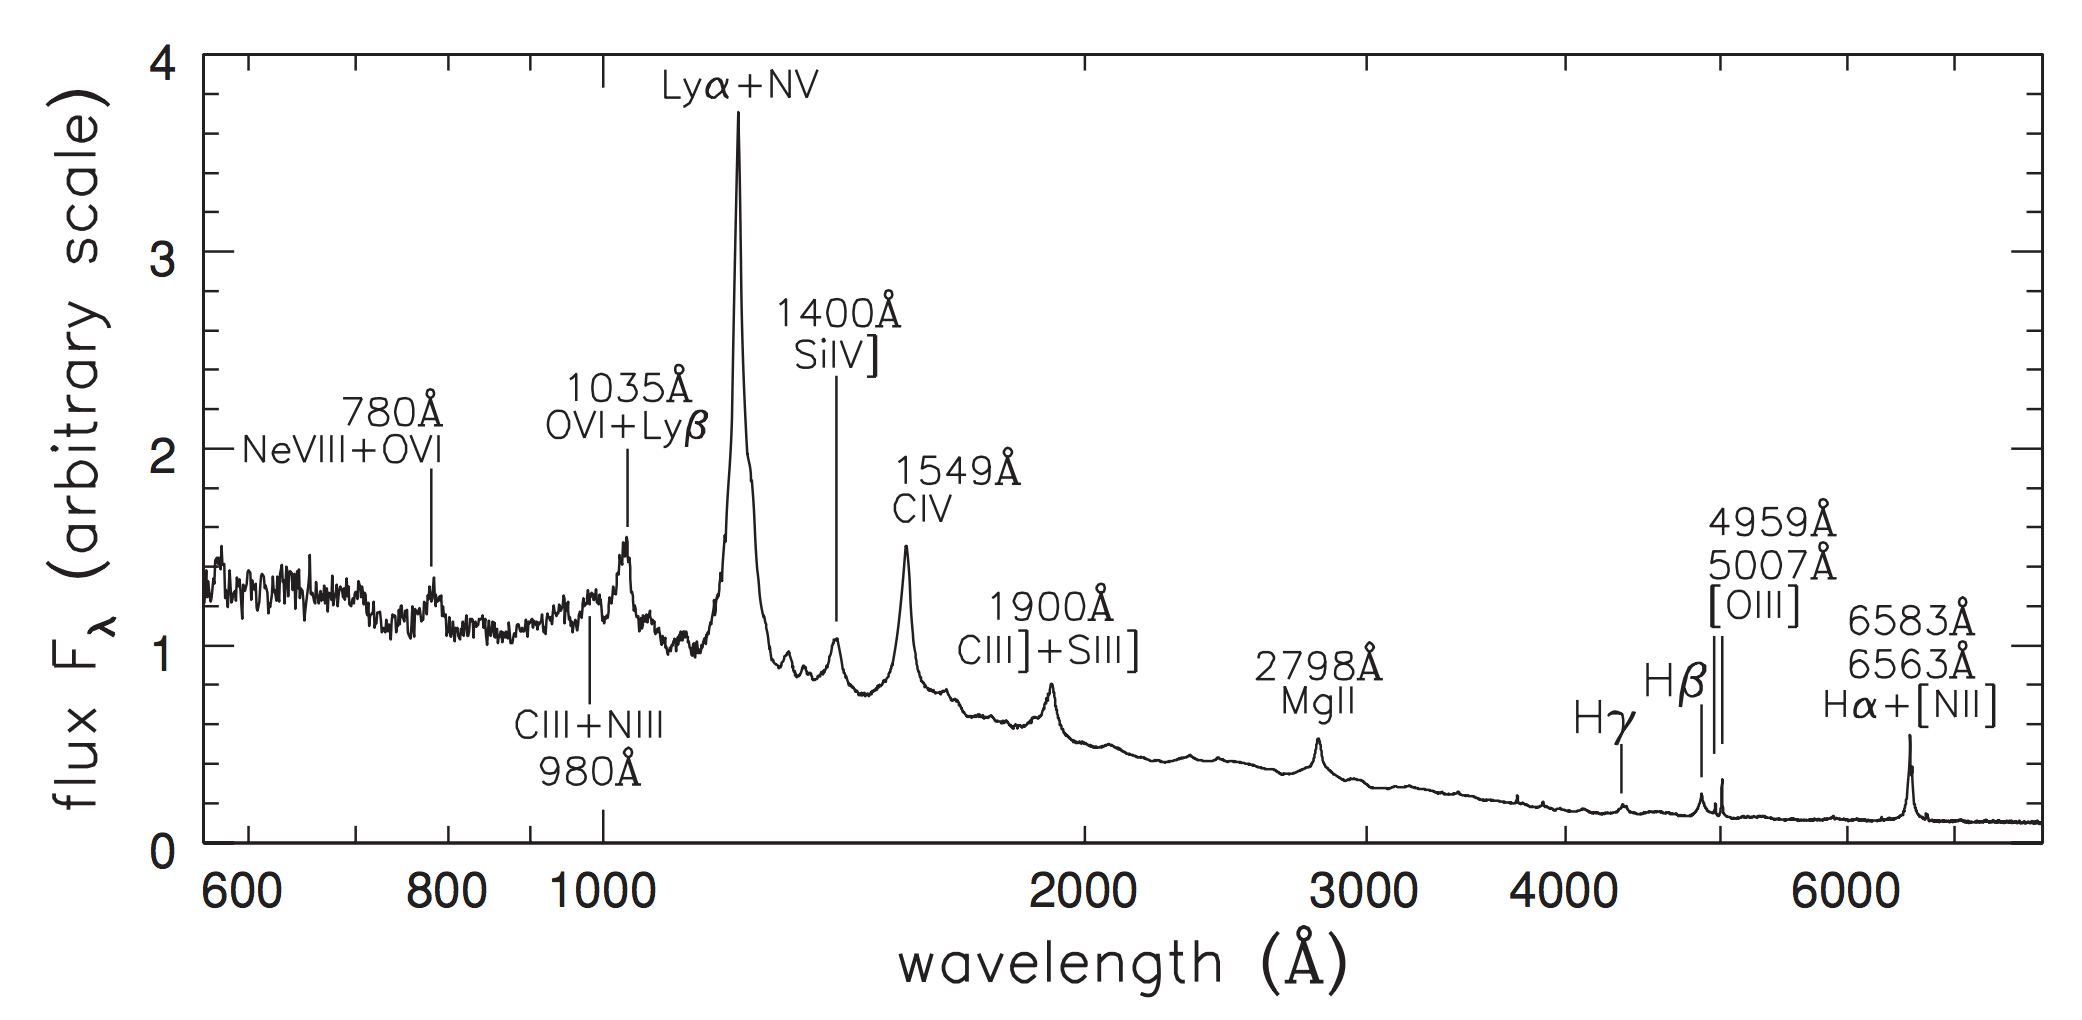
\includegraphics[width=16cm]{figures/QSO_radioquiet.png}
    \caption{\footnotesize{The ultraviolet and optical spectrum of an `average' radio-quiet quasar. Source: R.Telfer et al. 2002 Ap J 565, 773. Figure taken from Sparke \& Gallagher (2007).}}
    \label{fig:qsoradioquiet}
\end{figure}

{\noindent}Quasars contain narrow emission lines and, in most case, broad emission lines that are the result of photoionization by the continuum radiation. Narrow emission lines originate outside the opaque torus in the narrow-line region, whereas broad emission lines are formed in the broad-line region that is relatively close to the center. Typically, the spectrum of a high-redshift quasar contains a strong Lyman-$\alpha$ emission line produced by the quasar itself, and perhaps some $50$ Ly$\alpha$ absorption lines at shorter wavelengths (i.e., bluer than $1216$\AA); see Figure \ref{fig:lymanalphaforest}. Each one of these lines is from a different intergalactic cloud of hydrogen (and presumably helium) encountered by the quasar's continuum radiation on its journey to Earth.

\subsubsection{Additional context}

{\noindent}The first quasars (for `quasi-stellar radio source') were discovered as `radio galaxies with no galaxy'. They appeared point-like in optical photographs; only their enormous redshifts betrayed that they were not Galactic stars. Rather, they were gigaparsecs distant, and hence extremely luminous. Subsequently `radio-quiet' quasars, called quasi-stellar objects, or QSOs, were found by searching for objects that appeared stellar, but emitted too strongly at infrared or ultraviolet wavelengths relative to their brightness in visible light. Radio-quiet QSOs outnumber radio-loud quasars by at least a factor of 30; both are now believed to be variants of the same type of object, so we use the term `quasar' to include the QSOs. In the 1980s, deep images of nearby quasars showed us that they were in fact the bright nuclei of galaxies, so luminous as to outshine the surrounding stars. Most astronomers now regard quasars as more powerful versions of a Seyfert nucleus. Quasars cover a very wide range in luminosity; the most powerful are also the rarest.

{\noindent}Quasars are the most luminous members of the class of AGNs. The optical and ultraviolet spectrum of a quasar typically shows strong broad emission lines characteristic of moderately dense gas (Figure \ref{fig:qsoradioquiet}). The widths of the lines correspond to the Doppler shifts expected from emitting gas travelling at speeds $\sim10,000\,{\rm km\,s^{-1}}$. These emitting clouds are moving much faster than the galaxy's stars, which typically orbit at a few hundred kilometers per second. Many AGN are variable, changing their luminosity substantially within a few months, days, or even hours. The emission lines also strengthen and decline, within a few days or weeks. To allow such fast variability, both broad lines and continuum radiation must come from a region no more than a few light-weeks across.

{\noindent}Interestingly, the flux of the source varies at nearly all frequencies, where the variability time-scale differs among the objects and also depends on the wavelength. As a rule, it is found that the variability time-scale of the observed radiation is smaller, and its amplitude larger, at higher frequencies. The optical spectrum is very blue; most quasars at redshifts $z\lesssim2$ have $(U-B)<-0.3$ (for comparison, only hot white dwarfs have a similarly blue color index). Besides this blue continuum, very broad emission lines are characteristic of the optical and UV spectrum. Some of them correspond to transitions of very high ionization energy.

{\noindent}The continuum spectrum of a quasar can often be described, over a broad frequency range, by a power law of the form

\begin{align*}
    S_\nu \propto \nu^{-\alpha},
\end{align*}

{\noindent}where $\alpha$ is the spectral index. A spectral index of $\alpha-0$ corresponds to a flat spectrum, whereas $\alpha=1$ describes a spectrum in which the same energy is emitted in every logarithmic frequency interval. Incidentally, the energy distribution seen in Fig \ref{fig:qsoradioquiet} corresponds approximately to the latter case, over more than ten orders of magnitude in frequency, although over smaller frequency ranges, the spectral shape differs markedly from $\alpha=1$.

{\noindent}Quasars emit an excess of ultraviolet light relative to stars and so are quite blue in appearance. This UV excess is indicated by the big blue bump between roughly $10^{14}\,{\rm Hz}$ and $10^{16}\,{\rm Hz}$ which is a feature of most (but not all) quasar spectra. Absorption lines may also be present in some quasar spectra. In particular, Doppler broadened absorption lines, found in up to $10\%$ of quasar spectra, originate from sources with speeds exceeding $10^4\,{\rm km\,s^{-1}}$. These lines are believed to be associated with the quasar itself. Many additional narrow absorption lines are typically seen in the spectra with high redshifts ($z>2.2$) due to the Lyman series of hydrogen and metals such as C IV and Mg II. These lines would normally appear at ultraviolet wavelengths, but have been redshifted into the visible spectrum by the recessional velocity of the absorbing material. The absorption lines of a given quasar can be placed into different groups that share common redshifts. Furthermore, the redshifts of these narrow absorption lines are nearly always less than the redshift of the quasar's emission lines. The various groupings of lines are thought to arise from clouds of intervening material that lie between the quasar and Earth.

{\noindent}The spectra of high redshift quasars always displays a large number of narrow absorption lines superimposed on the quasar's continuous spectrum (these lines are in addition to any broad absorption lines that are associated with the quasar itself). These narrow lines are formed when the light from a quasar passes through material that happens to lie along the line of sight. If the absorbing material is far from Earth, its recessional motion will cause these absorption lines to be strongly redshifted. Furthermore, if the light passes through more than one cloud or galactic halo during its trip to Earth, different sets of absorption lines will be seen.

{\noindent}There are two classes of narrow absorption lines in quasar spectra:

\begin{itemize}
    \item The \textbf{Lyman-}$\boldsymbol{\alpha}$ \textbf{forest} is a dense thicket of hydrogen absorption lines. These lines are believed to be formed in intergalactic clouds and display a variety of redshifts. Absorption by primordial ionized helium (He II) has also been detected.
    \item Lines are also formed by \textbf{ionized metals}, primarily carbon (C IV) and magnesium (Mg II), together with silicon, iron, aluminum, nitrogen, and oxygen. The mix of elements is similar to that found in the ISM of the MW, indicating that the material has been processed through stars and enriched in heavy elements. These lines are thought to be formed in the extended halos or disks of galaxies found along the line of sight to the quasar.
\end{itemize}

{\noindent}Most of these lines are normally found at UV wavelengths, when the absorbing material is moving at a small fraction of the speed of light relative to Earth (i.e., has a small redshift). They are rarely seen from the ground because Earth's atmosphere absorbs most UV to visible wavelengths, where the atmosphere is transparent. For this reason, these absorption lines are seen from the ground only in the spectra of highly redshifted quasars.

{\noindent}Typically, the spectrum of a high-redshift quasar contains a strong Lyman-$\alpha$ emission line produced by the quasar itself, and perhaps some $50$ Ly$\alpha$ absorption lines at shorter wavelengths (i.e., smaller redshifts); see Figure \ref{fig:lymanalphaforest}. Each one of these lines is from a different intergalactic cloud of hydrogen (and presumably helium) encountered by the quasar's continuum radiation on its journey to Earth. The Ly$\alpha$ line profile can be used to calculate the column density of neutral hydrogen atoms in the cloud that produced each line, typically $10^{-18}\,{\rm m^{-2}}$. In other words, a hollow tube having a cross-sectional area of $1\,{\rm m^2}$ that crossed completely through the cloud would contain $10^{18}$ neutral hydrogen atoms. Such a could would be extremely transparent to the UV radiation that is normally present throughout space. As a result, this UV background can penetrate the cloud and keep it completely ionized. Calculations indicate that only one hydrogen atom in $10^5$ remains neutral in the cloud and is capable of absorbing a UV photon.

The comoving space density of intergalactic clouds appears to have been greater in the past than it is today, so the number of clouds has been decreasing as the Universe ages. A statistical analysis of the clouds' redshifts reveals little evidence that the clouds tend to be grouped in clusters. Instead, they appear to be distributed randomly throughout space. In particular, there do not appear to be large voids in the distribution of these intergalactic clouds similar to those seen in the distribution of galaxies. The distribution of He II is similarly uncertain.

\begin{figure}[t]
    \centering
    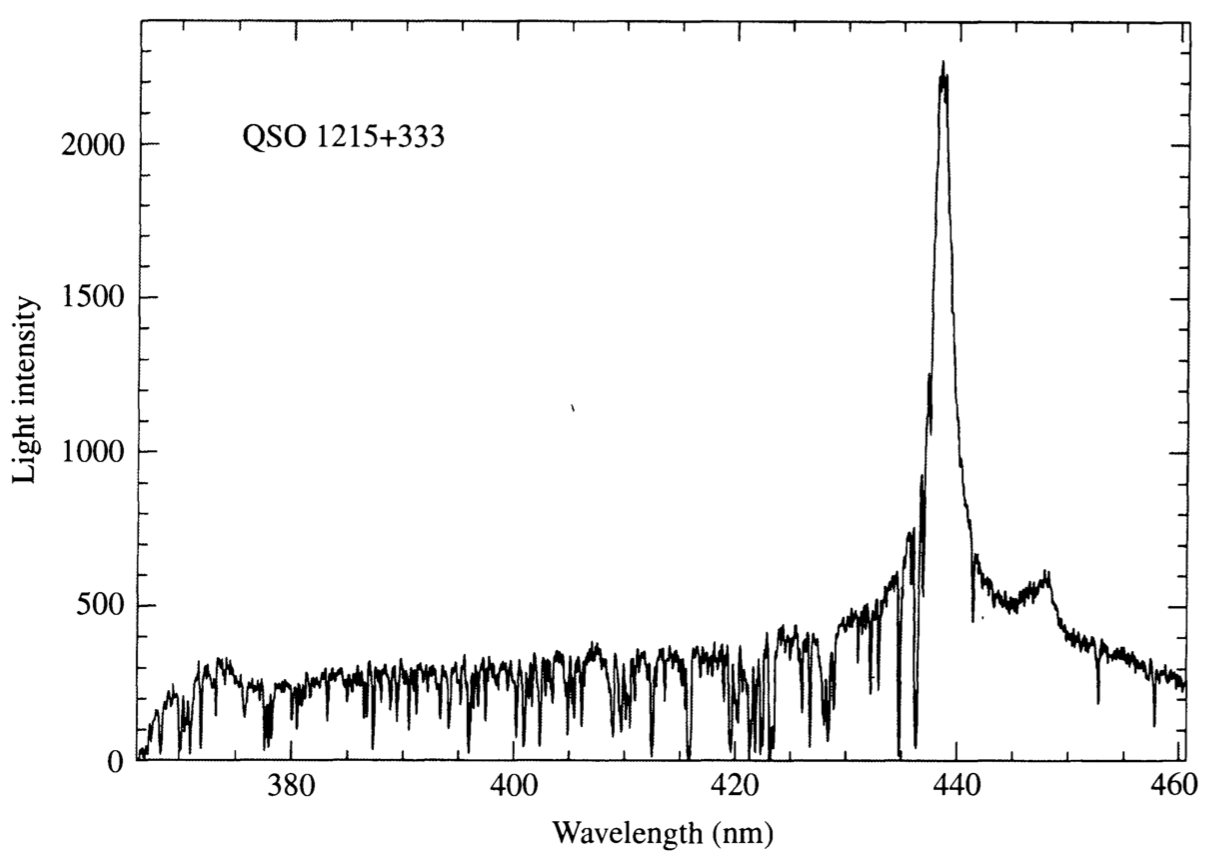
\includegraphics[width=14cm]{figures/LymanAlphaForest.png}
    \caption{\footnotesize{The strong Ly$\alpha$ emission line in the spectrum of QSO $1215+333$, with the Ly$\alpha$ forest of absorption lines at shorter wavelengths. Adapted from a figure courtesy of J. Bechtold, Steward Observatory, University of Arizona. Figure taken from Carroll \& Ostlie (2007).}}
    \label{fig:lymanalphaforest}
\end{figure}

% --------------------------------------------------------------
%               11. 
% --------------------------------------------------------------

\newpage
\subsection{Question 11}

Sketch the SED from the radio to gamma of extragalactic radiation on large angular scales. Describe the source and emission mechanism for each feature.

\subsubsection{Short answer}

\begin{figure}[h]
    \centering
    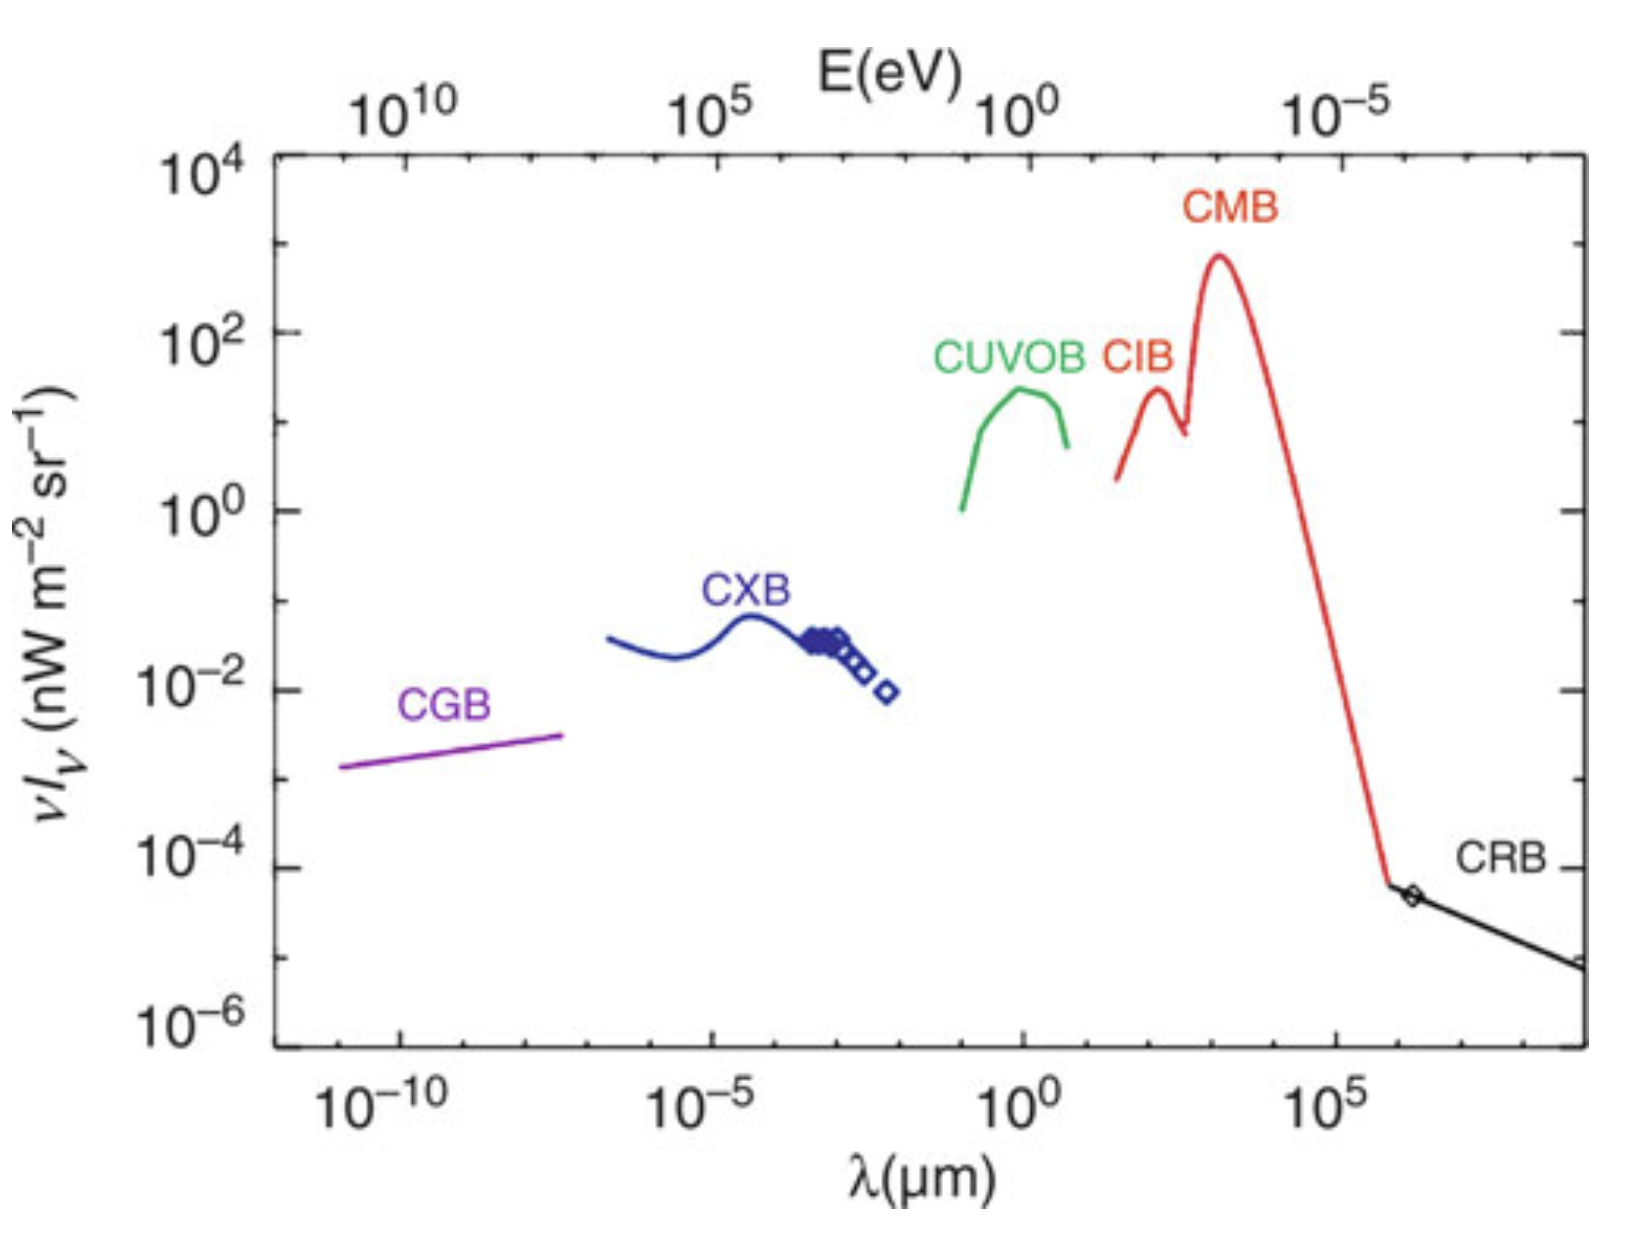
\includegraphics[width=14cm]{figures/DiffuseBackground.png}
    \caption{\footnotesize{Spectrum of cosmic background radiation, plotted as $\nu I_\nu$ versus wavelength so that the curve shows the intensity per logarithmic frequency interval. Besides the CMB, background radiation exists in the radio domain (cosmic radio background, CRB), in the infrared (CIB), in the optical/UV (CUVOB), in the X-ray (CXB), and at gamma-ray energies (CGB). With the exception of the CMB, all of these backgrounds can be understood as a superposition of the emission from discrete sources. Source: M.G. Hauser \& E. Dwek 2001, ARA\&A 39, 249, Fig.1. Figure taken from Schneider (2006).}}
    \label{fig:diffusebackground}
\end{figure}

\subsubsection{Additional context}

Figure \ref{fig:diffusebackground} shows the spectrum of cosmic background radiation, plotted as $\nu I_\nu$ versus wavelength so that the curve shows the intensity per logarithmic frequency interval. Following the terminology of the CMB, these are called background radiation as well. However, the name should not imply that it is a background radiation of cosmological origin, in the same sense as the CMB. The neutrino background that should be present as a relic from the early epochs of the Universe, in the form of a thermal distribution of all three neutrino families with $T\approx1.9\,{\rm K}$, is likely to remain undiscovered for quite some time due to the very small cross section of these low energy neutrinos.

{\noindent}In the present context, we simply denote the flux in a specific frequency domain, averaged over sky position at high Galactic latitudes, as background radiation. Thus, when talking about e.g., the optical background, we refer to the sum of the radiation of all galaxies and AGNs per solid angle. The interpretation of such a background radiation depends on the sensitivity and the angular resolution of the telescopes used. Imagine, for instance, observing the sky with an optical camera that has an angular resolution of only one arcminute. A relatively isotropic radiation would then be visible at most positions in the sky, featuring only some very bright or very large sources. Thus, the background can be decomposed into a `resolved' component, which can be attributed to individually identified sources, and the unresolved component. On improving the angular resolution, more and more individual sources become visible, so that a larger fraction of the background radiation is resolved. At optical wavebands, the Hubble Deep Fields have resolved essentially all of the background into individual sources. In analogy to this, one may wonder whether the CXB or the CIB can likewise be understood as a superposition of radiation from discrete sources.

{\noindent}\textbf{Cosmic gamma-ray background (CGB)}: Mostly from blazars (beamed synchrotron radiation.).

{\noindent}\textbf{Cosmic x-ray background (CXB)}: The first X-ray experiment in astronomy, a balloon flight in 1962, discovered a diffuse X-ray emission across the sky, confirmed by the first X-ray satellites which discovered not only a number of extragalactic X-ray sources (such as AGNs and clusters of galaxies), but also an apparently isotropic radiation component. The spectrum of the cosmic X-ray background (CXB) is a very hard (i.e., flat) power law, cut off at an energy above $40\,{\rm keV}$, which can roughly be described by

\begin{align*}
    I_\nu \propto E^{-0.3}\exp\left(-\frac{E}{E_0}\right),
\end{align*}

{\noindent}with $E_0\sim40\,{\rm keV}$. 

{\noindent}Initially, the origin of this radiation was unknown, since its spectral shape was different from the spectra of sources that were known at that time. For example, it was not possible to obtain this spectrum by a superposition of the spectra of known AGNs. ROSAT, with its substantially improved angular resolution compared to earlier satellites (such as the Einstein observatory), conducted source counts at much lower fluxes, based on some very deep images. From this, it was shown that at least 80\% of the CXB in the energy range between $0.5$ and $2\,{\rm keV}$ is emitted by discrete sources, of which the majority are AGNs. Hence it is natural to assume that the total CXB at these low X-ray energies originates from discrete sources, and observations by XMM-Newton and Chandra have confirmed this.

{\noindent}However, the X-ray spectrum of normal AGNs is different from that seen by the CXB, namely it is considerably steeper(about $S_\nu\propto\nu^{-S0.7}$). Therefore, if these AGNs contribute the major part of the CXB at low energies, the CXB at higher energies cannot possibly be produced by the same AGNs. Subtracting the spectral energy of the AGNs found by ROSAT from the CXB spectrum, one obtains an even harder spectrum, resembling very closely that of thermal bremsstrahlung. Therefore, it was supposed for a long time that the CXB is, at higher energies, produced by a hot intergalactic gas at temperatures of $k_BT\sim30\,{\rm keV}$. This model was excluded, however, by the precise measurement of the thermal spectrum of the CMB by COBE, showing that the CMB has a perfect blackbody spectrum. If a postulated hot intergalactic gas were able to produce the CXB, it would cause significant deviations of the CMB from the Planck spectrum, namely by the inverse Compton effect (the same effect that causes the SZ effect in clusters of galaxies). Thus, the COBE results clearly ruled out this possibility.

{\noindent}Deep observations with Chandra and XMM (e.g., in the CDFS) have finally resolved most of the CXB also at higher energies. From source counts performed in such fields, more than 75\% of the CXB in the energy range of $2\,{\rm keV}<E<10\,{\rm keV}$ could be resolved into discrete sources. Again, most of these sources are AGNs, but typically with a significantly harder (i.e., flatter) spectrum than the AGNs that are producing the low-energy CXB. Such a flat X-ray spectrum can be produced by photoelectric absorption of an intrinsically steep power law spectrum, where photons closer to the ionization energy are more efficiently absorbed than those at higher energy. According to the classification scheme of AGNs, these are Type 2 AGNs, thus Seyfert 2 galaxies and QSOs with strong intrinsic self-absorption. We should recall that Type 2 QSOs have only been detected by Chandra -- hence, it is no coincidence that the same satellite has also been able to resolve the high-energy CXB.

{\noindent}However, at even higher energies most of the CXB was still unaccounted for -- even the observed Type-2 AGNs could not account for it. It thus seems that there is a population of sources in the Universe which dominate the X-ray emission at high energies, still escape the observations at low X-ray frequencies. These could be heavily obscured AGNs, where only the hard X-rays manage to escape the emitting region. With the X-ray telescope onboard the Swift satellite, a significant number of such heavily obscured AGNs were found. Their estimated number density, together with their spectral energy distribution, make it plausible that they are the missing population of `hidden black holes' responsible for the hard CXB.

{\noindent}\textbf{Cosmic optical/ultraviolet background (CUVOB)}: Thermal emission from stars.

{\noindent}\textbf{Cosmic infrared background (CIB)}: The first point to note from Figure \ref{fig:diffusebackground} is the relatively flat energy distribution between the UV- and the mm-regime. Since both the UV-radiation and the far-IR radiation originate almost entirely from star-formation, the flat energy distribution implies that essentially half of the energetic photons emitted from newly-formed stars are absorbed by dust and reradiated in the FIR. Hence, estimates of the star formation activity from UV-flux alone will on average be biased low by 50\%. Observations of background radiation in the infrared are very difficult to accomplish, in particular due to the thermal radiation from the instruments and the zodiacal light. However, the DIRBE and FIRAS instruments onboard COBE provided a measurement of the CIB. The question now is whether the CIB can be understood as well as being due solely to individual sources.

{\noindent}Since mid- and far-IR observations are only possible from space, finding the answer to that question is challenging. Infrared observatories in space have a rather small aperture which, together with the long wavelength, yields a rather large point-spread function (PSF). This implies that when one observes to low flux limits, where the mean angular separation of sources on the sky becomes comparable to the size of the PSF, these sources can not be separated. This yields a lower flux limit for the detection of individual sources, called the confusion limit. The smaller the telescope, the shallower is the confusion limit reached. For example, the flux limit down to which individual sources could be identified with the Spitzer satellite at $160\,\mu{\rm m}$ corresponds to only 7\% of the CIB at this wavelength. The much larger mirror on the Herschel satellite lowered the confusion limit such that individual sources can be identified which account for about 52\% of the CIB. Going to larger wavelength, the confusion limit is even more severe.

{\noindent}However, one can dig deeper into the source counts with a technique called stacking. Taking the position of sources detected at some smaller wavelength (where the confusion limit is fainter), and adding up the flux in the longer wavelength band around all these positions, one obtains the mean long-wavelength flux of these sources. With this method, one will miss all fainter sources which do not have a detected counterpart in the short-wavelength input catalog, so that wavelength should be selected carefully. Given the characteristic spectrum of FIR-bright sources, one expects that most of the sources radiating in the FIR will have an appreciable flux at $24\,\mu{\rm m}$. Since Spitzer was particularly sensitive at this wavelength, the corresponding source catalog is best for a stacking analysis. Furthermore, if the redshifts of the sources selected at $24\,\mu{\rm m}$ is known, the stacking analysis can be used to determine the redshift distribution of the contributions to the CIB in the FIR. With stacking, the source counts can be followed to about three times lower flux than the confusion limit of individual sources permits.

{\noindent}\textbf{Cosmic microwave background (CMB)}: The cosmic microwave background (CMB) is a remnant of the early hot phase of the Universe, namely thermal radiation from the time before recombination. 

{\noindent}\textbf{Cosmic radio background (CRB)}: Synchrotron radiation, quasars, radio supernovae, and star forming galaxies.

% --------------------------------------------------------------
%               12. 
% --------------------------------------------------------------

\newpage
\subsection{Question 12}

What are AGNs? Describe different observational classes of them and how they may relate to each other.

\subsubsection{Short answer}

AGN are active galactic nuclei located at the center of active galaxies with very luminous non-thermal synchrotron emission. 


\begin{table}[h]
\caption{A summary of AGN classes. Table taken from Carroll \& Ostlie (2007).}
\begin{tabular}{lll}
\hline
Class & Sub-class & Description \\
\hline
Seyferts       & Type 1 & Broad and narrow emission lines; weak radio emission; X-ray \\
               & & emission; spiral galaxies; variable \\
               & Type 2 & Narrow emission lines only; weak radio emission; weak X-ray\\
               & & emission; spiral galaxies; not variable \\
QSOs           & Radio loud & Broad and narrow emission lies; strong radio emission; \\
               & (QSR) & some polarization; FR II; variable \\
               & Radio quiet & Broad and narrow emission lines; weak radio emission; \\
               & (QSO) & weak polarization; variable \\
Radio galaxies & Broad line & Broad and narrow emission lines; strong radio emission; \\
               & (BLRG) & FR II; weak polarization; elliptical galaxies; variable \\
               & Narrow line & Narrow emission lines only; strong radio emission; FR I \\
               & (NLRG) & and FR II; no polarization; elliptical galaxies; not variable \\
Blazars        & BL Lacs & Almost devoid of emission lines; strong radio emission; \\
               & & strong polarization; rapid variability; 90\% in ellipticals \\
               & OVV quasars & Broad and narrow emission lines; strong radio emission; \\
               & & strong polarization; rapid variability; much more luminous \\
               & & than BL Lacs \\
ULIRGs         &  & Possibly dust-enshrouded quasars, alternatively may be \\
               &  & starburst phenomena \\
LINERs         &  & Similar to low-luminosity Seyfert 2; low ionization emission \\
               &  & lines; in many (perhaps majority of) spiral galaxies; \\
LINERs         &  & alternatively may be starburst phenomena or HII region emission
\end{tabular}
\end{table}

\subsubsection{Additional context}

A wide range of objects are subsumed under the name AGN, all of which have in common strong non-thermal emission in the core of a galaxy (host galaxy). It is important to keep in mind that the frequency range in which sources are studied affects the source classification. The classification of AGNs is very confusing at first glance. Different classes refer to different appearances of AGNs but do not necessarily correspond to the physical nature of these sources. Similarly, the properties of the emission of AGNs in different wavebands (such as radio or gamma-rays) can differ most strongly. However, the large variety of appearances of AGNs can be understood, at least to a first approximation, by geometric considerations. The emission of an AGN is not isotropic; the flow of material which causes the energy release near the central black hole occurs in the form of a disk (the accretion disk), which defines a pair of preferred directions (i.e., those perpendicular to the plane in which the disk lies). In the context of unified models, the way an AGN appears to us depends strongly on the angle between this disk axis and the line-of-sight to the source.

{\noindent}In Figure \ref{fig:agn}, this geometric picture of an AGN is sketched. The different green arrows indicate different lines-of-sight to observers, and they are labeled with the characteristic AGN class the corresponding observer will see. In the upper half of the figure, it is assumed that the AGN produces strong jets, whereas in the lower part, weaker jets (or none at all) are assumed.\footnote{As is often the case with these figures, this schematic depicts two very different AGN cases -- one with a radio loud jet and one without. No such AGN can have one jet on one side and not the other!} With this picture in mind, we shall now describe the various types of AGNs. Surrounding the central supermassive black hole is an accretion disk which emits the bulk part of the optical and UV continuum emission. The central region around the accretion disk is the source of most of the X-ray radiation. Gas clouds above and below the accretion disk are responsible for the broad emission lines. In the plane of the disk, a distribution of gas and dust is present, which can absorb radiation from the inner region of the AGN; this obscuring material is sometimes depicted as a torus, though its geometry is probably more complicated. Nevertheless, the appearance of the AGN depends on whether the observer is located near the plane of the disk -- where radiation is partly absorbed by the material in the torus -- or placed in a direction closer to the axis of the disk. This concerns in particular the broad line emission, which may be fully obscured for an observer in the plane of the disk. In contrast, the gas responsible for the narrow emission lines is located at much larger distances from the black hole, so that it cannot be fully hidden by the obscuring torus. 

\begin{figure}[t]
    \floatbox[{\capbeside\thisfloatsetup{capbesideposition={right,top},capbesidewidth=4cm}}]{figure}[\FBwidth]
    {\caption{\footnotesize{Sketch of our current understanding of the unification of AGN types. The accretion disk is surrounded by a thick `torus' containing dust which thus obscures the view to the center of the AGN. When looking from a direction near the plane of the disk, a direct view of the continuum source and the BLR is blocked, whereas it is directly visible from directions closer to the symmetry axis of the disk. The difference between Seyfert 1 (and BLRG) and Seyfert 2 (and NLRG) is therefore merely a matter of orientation relative to the line-of-sight. If an AGN is seen exactly along the jet axis, it appears as a blazar. Credit: NASA. Figure taken from Schneider (2006).}}
    \label{fig:agn}}
    {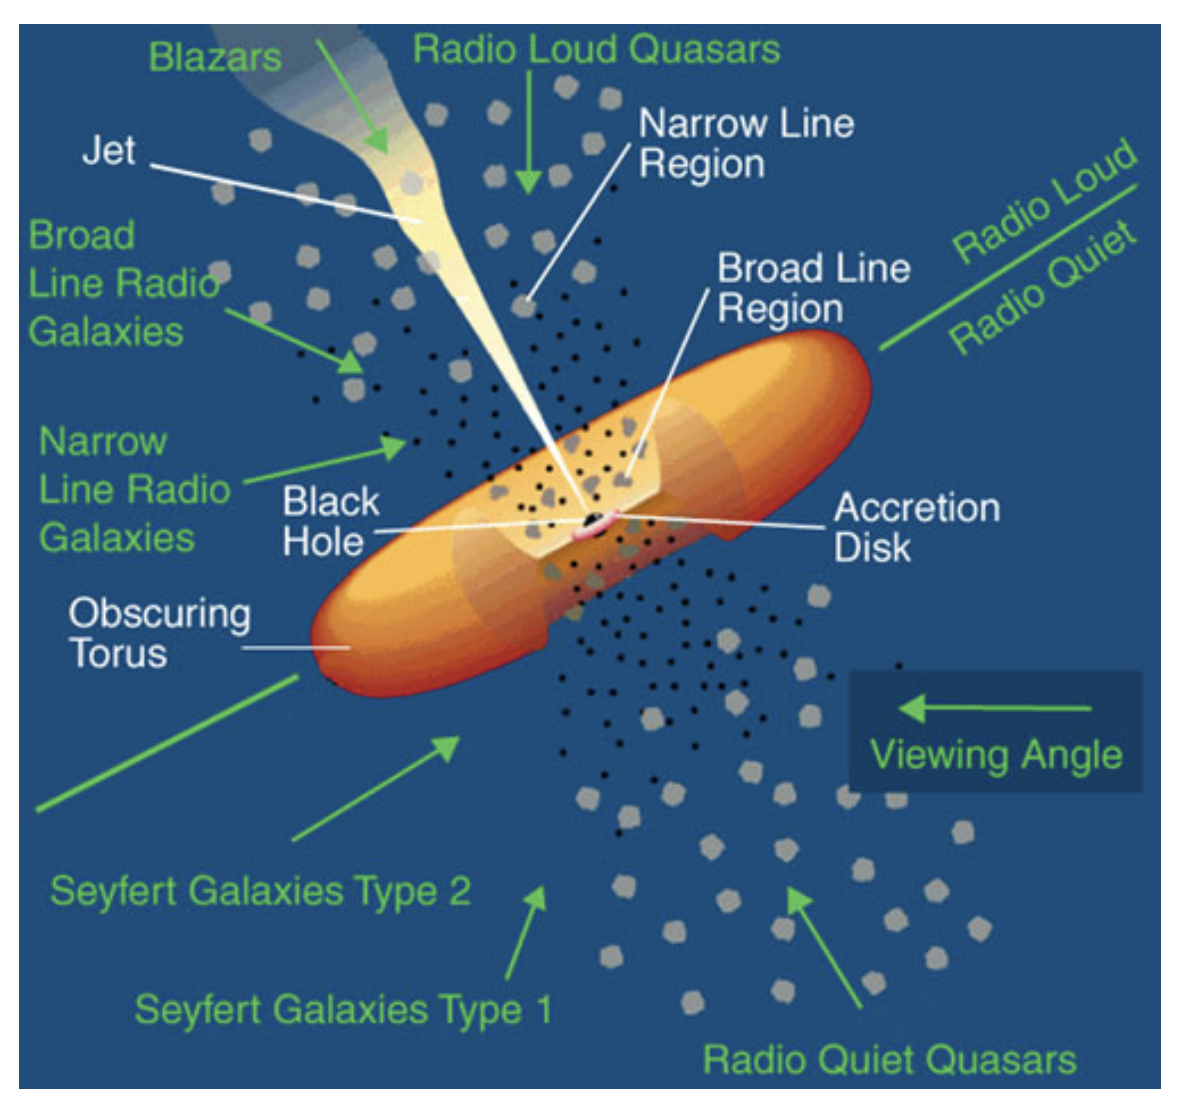
\includegraphics[width=10cm]{figures/AGN.png}}
\end{figure}

{\noindent}The radio jets are launched very close to the central black hole along the direction of the disk axis. The emission from these jets is highly anisotropic, because the velocity in the inner part of the jets is close to the speed of light; then, according to the theory of Special Relativity, the jet emission is strongly beamed in the direction of jet motion. This implies that the appearance of the jet depends on how close the line-of-sight to an observer is to the jet axis. If the jet points almost directly at the observer, the jet emission can outshine all the other radiation from the AGN. 

{\noindent}The QSOs are the most luminous AGNs. Their core luminosity can be as high as a thousand times that of an $L^*$  galaxy. Therefore they can outshine their host galaxy and appear point-like on optical images. For QSOs of lower $L$, their host galaxies were identified and spatially resolved with the HST. According to our current understanding, AGNs are the active cores of galaxies. These galaxies are supposed to be fairly normal galaxies, except for their intense nuclear activity.

{\noindent}The unusually blue color of quasars suggested the possibility of searching for them not only with radio observations but also at optical wavelengths, namely to look for point-like sources with a very blue $U-B$ color index. These photometric surveys were very successful. In fact, many more such sources were found than expected from radio counts. Most of these sources are (nearly) invisible in the radio domain of the spectrum; such sources are called radio-quiet. Their optical properties are virtually indistinguishable from those of quasars. In particular, they have a blue optical energy distribution (of course, since this was the search criterion!), strong and broad emission lines, and in general a high redshift.

{\noindent}Apart from their radio properties, these sources appear to be like quasars. Therefore they were called radio-quiet quasars, or quasi-stellar objects, QSOs. Today this terminology is no longer very common because the clear separation between sources with and without radio emission is not considered valid any more. Radio-quiet quasars also show radio emission if they are observed at sufficiently high sensitivity. In modern terminology, the expression QSO encompasses both the quasars and the radio-quiet QSOs. About 10 times more radio-quiet QSOs than quasars are thought to exist.

{\noindent}In fact, there is as yet not a clear consensus in whether QSOs show a bimodal distribution in their ratio of radio-to-optical luminosity. Figure \ref{fig:qsoradiovsoptical} shows several different samples of AGN; in particular, optically-selected QSOs from the Palomar-Green survey (filled stars) and radio-loud QSOs (open circles). It seems that the ratio between radio and optical luminosity falls into two broad ranges, with a clear gap in between. Therefore, diagrams like that argue in favor of a bimodal distribution. However, this apparent division into two classes can at least partly be attributed to selection effects: the distribution of the radio-to-optical flux ratio depends on the selection of the QSO sample. Obviously, selecting them by their radio emission will favor those with a large $L_\mathrm{radio}/L_\mathrm{opt}$ ratio. Furthermore, the fraction of QSOs for which this ratio is large (i.e., which would be termed as radio-loud QSOs) depends on optical luminosity and on redshift: One finds a significantly higher radio-loud fraction amongst more luminous, and lower-redshift QSOs.

\begin{figure}[h]
    \floatbox[{\capbeside\thisfloatsetup{capbesideposition={right,top},capbesidewidth=4cm}}]{figure}[\FBwidth]
    {\caption{\footnotesize{Radio vs. optical luminosity of AGN, as measured at $5\,{\rm GHz}$ and in the B-band. Different types of AGNs are shown with different symbols: FR I radio galaxies (open triangles), Broad-Line Radio Galaxies (filled circles), radio-loud QSOs (open circles), Seyfert galaxies and LINERs (crosses), and a sample a $(U-B)$ colour-selected bright QSOs, the Palomar-Green sample (filled stars). Source: M. Sikora et al. 2007, Radio Loudness of Active Galactic Nuclei: Observational Facts and Theoretical Implications, ApJ 658, 815, p. 823, Fig. 1. Figure taken from Schneider (2006).}}
    \label{fig:qsoradiovsoptical}}
    {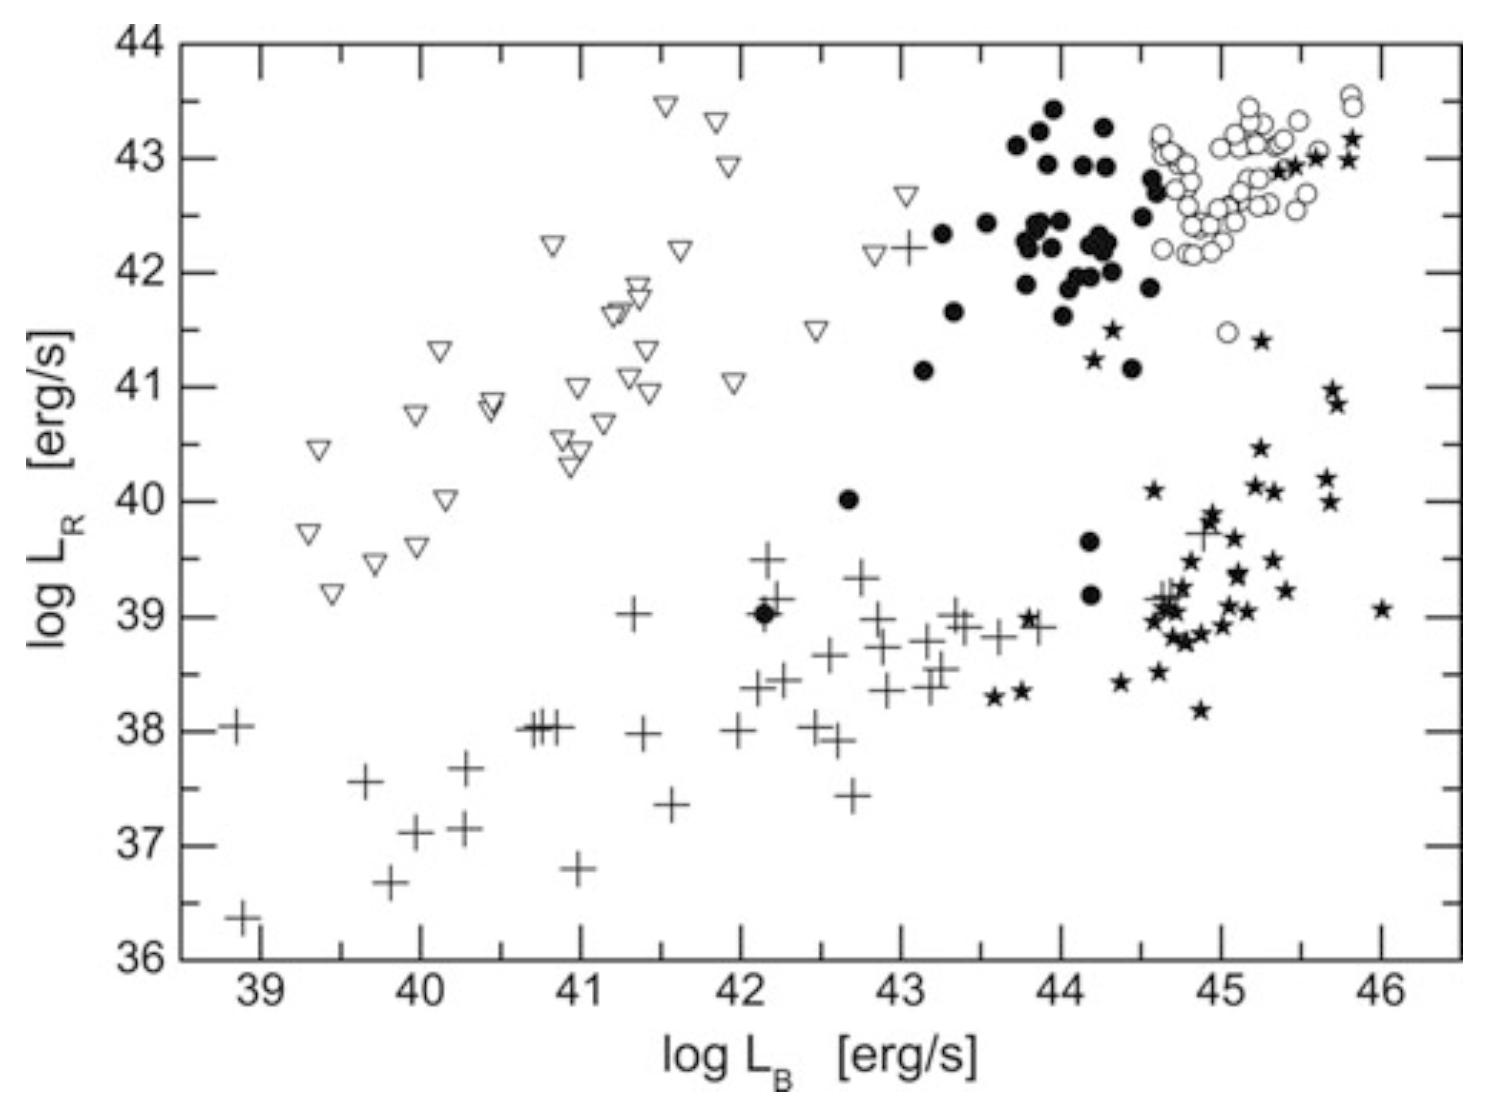
\includegraphics[width=12cm]{figures/QSO_radiovsoptical.png}}
\end{figure}

\subsubsection{Follow-up Questions}

\begin{itemize}
    \item What are the physical scales in this diagram? (Cross section of SMBH, accretion disk and jet.)
    \item How massive are SMBHs?
    \item Why is there a connection between bulge properties and SMBH mass?
    \item How do you determine over what range SMBH potential is important?
\end{itemize}


% --------------------------------------------------------------
%               13. 
% --------------------------------------------------------------

\newpage
\subsection{Question 13}

What are galaxy clusters? What are their basic properties (e.g., mass, size). List and explain three ways they can be detected.

\subsubsection{Short answer}

Clusters of galaxies are gravitationally bound systems of a hundred or more galaxies with diameters of $\sim\,{\rm Mpc}$ and masses of $\sim10^{13}-10^{14}\,{\rm M_\odot}$. Clusters predominantly contain early-type galaxies, so there is not much star formation taking place any more. Some clusters of galaxies seem to be rather circular in projection, others have a highly elliptical or irregular distribution of galaxies; some even have more than one center.

{\noindent}Detection methods include:

\begin{itemize}
    \item \textbf{X-ray emission}: Clusters of galaxies are strong sources of X-ray radiation. They contain hot gas, with temperatures ranging from $10^7$ up to $10^8\,{\rm K}$.
    \item \textbf{Sunyaev-Zeldovich effect}: The hot X-ray ICM gas inverse Compton scatters CMB photons which appears as a bright spot in the CMB and a deviation from a perfect $2.7\,{\rm K}$ CMB blackbody in that direction.
    \item \textbf{Weak gravitational lensing}: The angle of deflection of a background light source is directly proportional to the intervening mass of the galaxy cluster.
\end{itemize}

\subsubsection{Additional context}

The cluster of galaxies closest to us is the Virgo cluster, at a distance of $18\,{\rm Mpc}$; it is a cluster with an irregular galaxy distribution. The closest regular cluster is Coma, at a distance of $90\,{\rm Mpc}$. Coma contains about 1000 luminous galaxies, of which 85\% are early-type galaxies.

{\noindent}In 1933, Fritz Zwicky measured the radial velocities of the galaxies in Coma and found that their distribution around the mean has a dispersion of about $1000\,{\rm km\,s^{-1}}$. From the total luminosity of all its galaxies the mass of the cluster can be estimated. If the stars in the cluster galaxies have an average mass-to-light ratio ($M/L$) similar to that of our Sun, we would conclude $M=(M_\odot/L_\odot)L$. However, stars in early-type galaxies are on average slightly less massive than the Sun and thus have a slightly higher $M/L$. Thus, the above mass estimate needs to be increased by a factor of $\sim10$.

{\noindent}Zwicky then estimated the mass of the cluster by multiplying the luminosity of its member galaxies with the mass-to-light ratio. From this mass and the size of the cluster, he could then estimate the velocity that a galaxy needs to have in order to escape from the gravitational field of the cluster -- the escape velocity. He found that the characteristic peculiar velocity of cluster galaxies (i.e., the velocity relative to the mean velocity) is substantially larger than this escape velocity. In this case, the galaxies of the cluster would fly apart on a time-scale of about $10^9\,{\rm yr}$ (the time it takes a galaxy to cross through the cluster once) and, consequently, the cluster would dissolve. However, since Coma seems to be a relaxed cluster (i.e., it is in equilibrium and thus its age is definitely larger than the dynamical time scale of $10^9\,{\rm yr}$) Zwicky concluded that the Coma cluster contains significantly more mass than the sum of the masses of its galaxies. Using the virial theorem he was able to estimate the mass of the cluster from the velocity distribution of the galaxies. This was the first clear indicator of the existence of dark matter.

\begin{figure}[h]
    \centering
    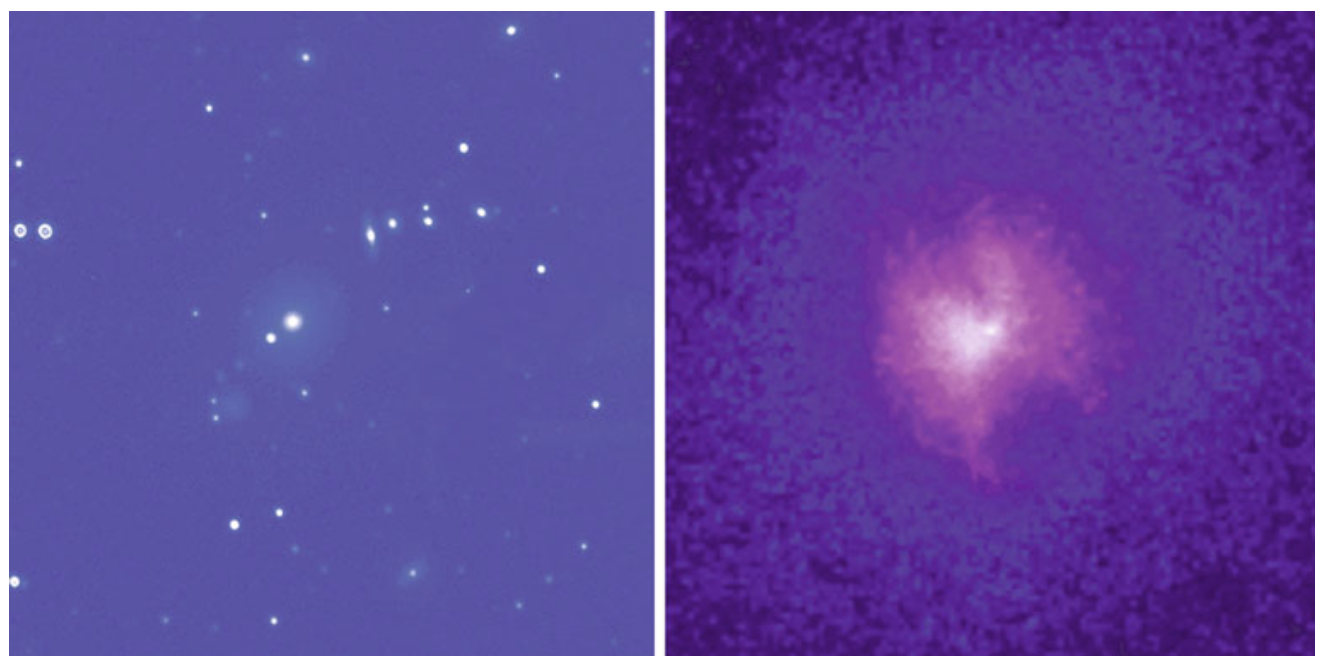
\includegraphics[width=14cm]{figures/HydraA.png}
    \caption{\footnotesize{The HydraA cluster of galaxies. The left-hand figure shows an optical image, the one on the right an image taken with the X-ray satellite Chandra. The cluster has a redshift of $z\approx0.054$ and is thus located at a distance of about $250\,{\rm Mpc}$. The X-ray emission originates from gas at a temperature of $40\times10^6\,{\rm K}$ which fills the space between the cluster galaxies. In the center of the cluster, the gas is cooler by about 15\%. Credit: Optical: B. McNamara, La Palma; X-ray: NASA/CXC/SAO. Figure taken from Schneider (2006).}}
    \label{fig:hydraa}
\end{figure}

{\noindent}X-ray satellites later revealed that clusters of galaxies are strong sources of X-ray radiation. They contain hot gas, with temperatures ranging from $10^7$ up to $10^8\,{\rm K}$ (Figure \ref{fig:hydraa}). This gas temperature is another measure for the depth of the cluster's potential well, since the hotter the gas is, the deeper the potential well has to be to prevent the gas from escaping via evaporation. Mass estimates based on the X-ray temperature result in values that are comparable to those from the velocity dispersion of the cluster galaxies. Whereas the X-ray emitting gas provides a further mass component of ordinary, baryonic matter (in fact, the X-ray emitting gas contains more mass than the stars in the cluster galaxies) the total mass of clusters exceeds that of stars and gas by a factor of about five, thus clearly confirming the hypothesis of the existence of dark matter in clusters (Figure \ref{fig:abell383}). A third method for determining cluster masses, the so-called gravitational lensing effect, utilizes the fact that light is deflected in a gravitational field. The angle through which light rays are bent due to the presence of a massive object depends on the mass of that object. From observation and analysis of the gravitational lensing effect in clusters of galaxies, cluster masses are derived that are in agreement with those from the two other methods. Therefore, clusters of galaxies are a second class of cosmic objects whose mass is dominated by dark matter.

\begin{figure}[h]
    \floatbox[{\capbeside\thisfloatsetup{capbesideposition={right,top},capbesidewidth=4cm}}]{figure}[\FBwidth]
    {\caption{\footnotesize{The cluster of galaxies Abell 383, as seen in optical light, superposed by an image taken at X-ray energies (purple) with the Chandra satellite observatory. The space between the galaxies is filled by a hot gas, with temperature of about 50 million degrees, which emits the energetic X-ray radiation. The cluster is at a redshift of $z=0.19$, corresponding to a distance of about $800\,{\rm Mpc}$, and has an estimated mass of $3\times10^{14}\,{\rm M_\odot}$. Credit: X-ray: NASA/CXC/Caltech/A. Newman et al./Tel Aviv/A. Morandi \& M. Limousin; Optical: NASA/STScI, ESO/VLT, SDSS. Figure taken from Schneider (2006).}}
    \label{fig:abell383}}
    {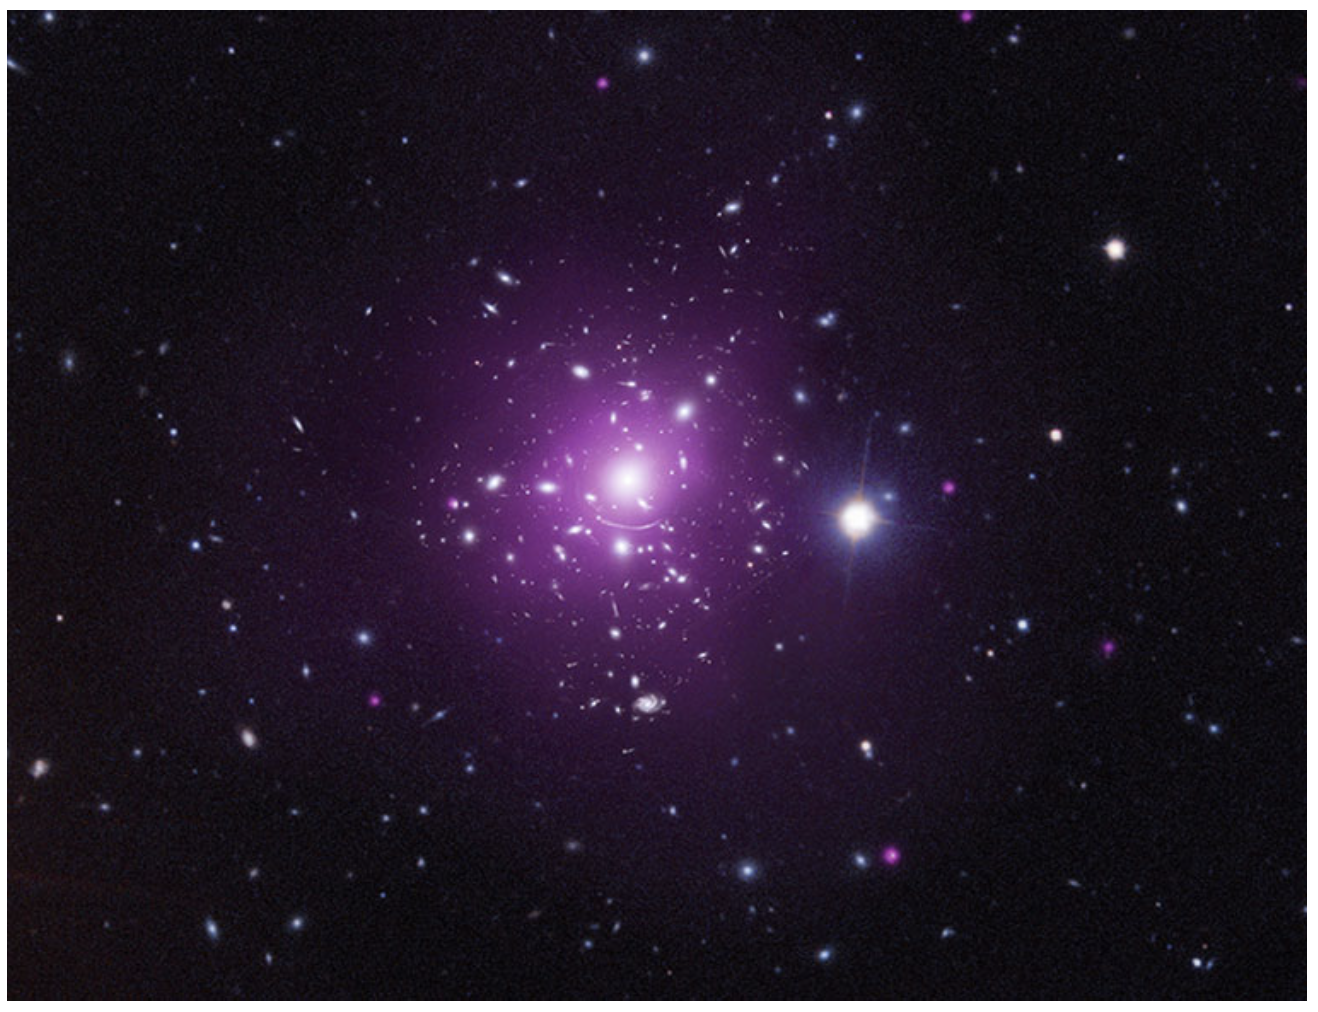
\includegraphics[width=10cm]{figures/Abell383.png}}
\end{figure}

{\noindent}Clusters of galaxies are cosmologically young structures. Their dynamical time-scale (i.e., the time in which the mass distribution in a cluster settles into an equilibrium state) is estimated as the time it takes a member galaxy to fully cross the cluster once. With a characteristic velocity of $v\sim1000\,{\rm km\,s^{-1}}$ and a diameter of $R\sim2\,{\rm Mpc}$ one thus finds

\begin{align*}
    t_\mathrm{dyn} \sim \frac{2R}{v} \sim 2\times10^9\,[{\rm yr}].
\end{align*}

{\noindent}the Universe is about $14\times10^9\,{\rm yr}$ old. During this time galaxies have not had a chance to cross the cluster many times. Therefore, clusters still contain, at least in principle, information about their initial state. Most clusters have not had the time to fully relax and evolve into a state of equilibrium that would be largely independent of their initial conditions. Comparing this with the time taken for the Sun to rotate around the center of the Milky Way (about $2\times10^8\,{\rm yr}$) galaxies thus have had plenty of time to reach their state of equilibrium.

{\noindent}Besides massive clusters of galaxies there are also galaxy groups, which sometimes contain only a few luminous galaxies. In fact, the number density of groups is far larger than that of clusters. Our Milky Way is part of such a group, the Local Group, which also contains M31 (Andromeda), a second luminous spiral galaxy besides the Milky Way, as well as some far less luminous galaxies such as the Magellanic Clouds. Some groups of galaxies are very compact (i.e., their galaxies are confined within a very small volume). Interactions between these galaxies cause the lifetimes of many such groups to be much smaller than the age of the Universe, and the galaxies in such groups will merge.

{\noindent}One of the most important discoveries of the UHURU X-ray satellite, launched in 1970, was the detection of X-ray radiation from massive clusters of galaxies. With the later Einstein X-ray satellite and more recently ROSAT, X-ray emission was also detected from lower-mass clusters and groups. Figure \ref{fig:comaxray} shows the Coma cluster of galaxies, observed with two different X-ray observatories. Although Coma was considered to be a fully relaxed cluster, distinct substructure is visible in its X-ray radiation. Clusters of galaxies are the brightest extragalactic X-ray sources besides AGNs. If an X-ray telescope is pointed away from the Galactic disk, about 85\% of the detected sources are AGNs, the remaining 15\% are clusters. In contrast to AGNs, for which the X-ray emission is essentially point-like, the X-ray emission of clusters is extended. Their characteristic luminosity is $L_X\sim10^{43}\,{\rm erg\,s^{-1}}$ up to $10^{45}\,{\rm erg\,s^{-1}}$ for the most massive systems. The fact that this X-ray emission is spatially extended implies that it does not originate from individual galaxies. The spatial region from which we can detect this radiation can have a size of $1\,{\rm Mpc}$ or even larger. In accordance with the extended nature of the X-ray source, no variability of its X-ray flux has been detected.

{\noindent}The assumption that the X-ray emission originates from a hot, diffuse gas (the ICM) was confirmed by the discovery of line emission in the X-ray spectrum of clusters. One of the most prominent lines in massive clusters is located at energies just below $7\,{\rm keV}$: it is the Lyman-$\alpha$ (``K$\alpha$'') line of 25-fold ionized iron (thus, of an iron nucleus with only a single electron). Slightly less ionized iron has a strong transition at somewhat lower energies of $E\sim6.4\,{\rm keV}$. Later, other lines were also discovered in the X-ray spectrum of clusters. As a rule, the hotter the gas is, thus the more completely ionized it is, the weaker the line emission. 

{\noindent}The spectral energy distribution of the X-rays leads to the conclusion that the emission process is optically thin thermal bremsstrahlung (free-free radiation) from a hot gas which is collisionally ionized. This radiation is produced by the acceleration of electrons in the Coulomb field of protons and atomic nuclei. Since an accelerated electrically charged particle emits radiation, such scattering processes between electrons and protons in an ionized gas yields emission of photons. From the spectral properties of this radiation, the gas temperature in galaxy clusters can be determined, which is, for clusters with mass between $\sim3\times10^{13}\,{\rm M_\odot}$ and $10^{15}\,{\rm M_\odot}$, in the range of $10^7\,{\rm K}$ to $10^8\,{\rm K}$, or $1$ to $10\,{\rm keV}$, respectively.

\begin{figure}[t]
    \centering
    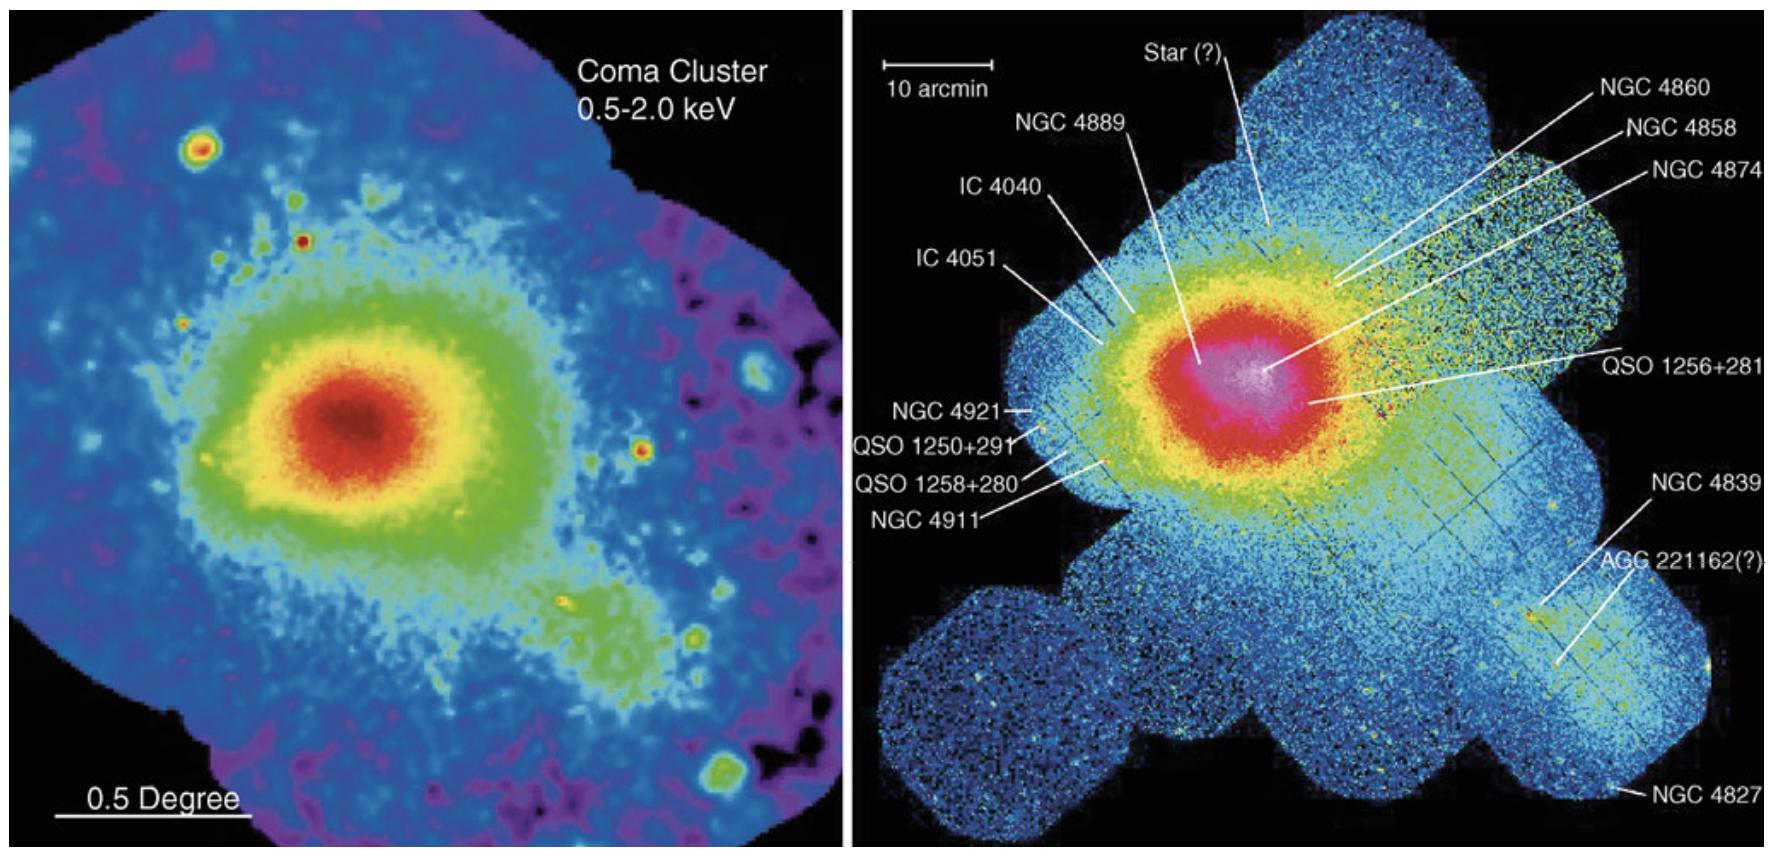
\includegraphics[width=14cm]{figures/ComaXray.png}
    \caption{\footnotesize{X-ray images of the Coma cluster, taken with the ROSAT-PSPC (left) and XMM-EPIC (right). The image size in the left panel is $2.7^\circ\times2.5^\circ$, much larger than what's seen in the optical. A remarkable feature is the secondary maximum in the X-ray emission at the lower right of the cluster center which shows that even Coma, long considered to be a regular cluster, is not completely in an equilibrium. Figure taken from Schneider (2006).}}
    \label{fig:comaxray}
\end{figure}

{\noindent}Typically, regular clusters have an X-ray luminosity $L_X$ and temperature that smoothly increases with cluster mass. In contrast, irregular clusters at a given mass can be either hotter or cooler than regular clusters. Irregular clusters are the result of a recent merging event, and their temperature depends on the stage of the merging process. In the initial phases of the merger, the kinetic energy is not yet thermalized, and thus the gas remains at approximately the same temperature it had before the merging event. Later on, the gas is heated by shock fronts in which the kinetic energy is transformed into internal energy of the gas (i.e., heat). In this phase, the gas temperature can be higher than that of a regular cluster of the same mass. Finally, the cluster settles into an equilibrium state. Indications of past merger events can be seen in substructures of the X-ray emitting gas; even for the Coma cluster, which is frequently considered a typical example of a relaxed cluster, signs of previous merger events can be detected.

{\noindent}The trend emerges that in clusters with a larger fraction of spiral galaxies, $L_X$ and $T$ are lower. Irregular clusters typically also have a lower central density of galaxies and gas compared to regular clusters. Clusters of galaxies with a dominant central galaxy often show a strong central peak in X-ray emission. The X-ray emission often deviates from axial symmetry, so that the assumption of clusters being roughly spherically symmetric is not well founded in these cases.

\subsubsection{Follow-up Questions}

\begin{itemize}
    \item (On the X-ray gas method of detection:) Where does it come from?
    \item (On the X-ray gas method of detection:) How do we see it / what is its emission mechanism?
    \item (On the X-ray gas method of detection:) How is the x-ray gas initially heated / why is it hot?
    \item Say more about galaxy interactions in clusters.
    \item Where is most of the mass in a galaxy cluster?
    \item What heats the IGM?
    \item Do optical surveys need redshift information to identify galaxy clusters?
    \item Describe how star formation changes throughout the cluster.
    \end{itemize}



% --------------------------------------------------------------
%               14. 
% --------------------------------------------------------------

\newpage
\subsection{Question 14}

What is star formation quenching? What is the evidence for it, and why is it thought to happen?

\subsubsection{Short answer}

Star formation quenching can either refer to the termination of SF activity or the process of maintaining a galaxy quiescent despite the presence of fresh fuel and inflows. Although feedback processes are often employed in theoretical studies, quenching does not necessarily mean feedback (i.e., there are quenching mechanisms that are not feedback mechanisms). Several mechanisms have been proposed to explain SF quenching, including but not limited to: `cosmological starvation', virial shock heating, AGN feedback, RAM pressure from satellite galaxies, stellar feedback, low SF efficiency, turbulence injection via AGN and magnetic fields, and cold gas being rapidly consumed.

\subsubsection{Additional context}

The term `quenching' has been used with two different meanings in the literature, to indicate either the termination of the star formation activity, or the process of maintaining a galaxy quiescent over its lifetime, despite the fresh fuel produced by stellar evolution and gas inflows. Given the substantially different timescales involved in the two processes, it remains under debate whether one single mechanism is responsible for both the onset and the maintenance of quenching. Archaeological evidence shows that the termination process must be particularly rapid for the most massive galaxies that would become present-day giant ellipticals, most of which were already quenched by a redshift of $z\approx2$. In theoretical studies, feedback by energetic sources is often used to quench star formation. Although closely related, quenching and feedback are not strictly equivalent: there are theoretical scenarios in which galaxies are quenched by processes that are not feedback mechanisms.

{\noindent}Over the years, numerous mechanisms have been proposed to explain the quenching of massive galaxies, including feedback from active galactic nuclei (AGNs), stellar feedback and gravitational effects. Given that these processes encompass several branches of astrophysics, it is not surprising that studies on the topic have suffered from inconsistent definitions and confusion in the literature.

{\noindent}Normally, stars form out of molecular gas of temperature $T<10^2\,{\rm K}$ that cooled and settled from warm and hot gas within the halo ($T=10^3-10^6\,{\rm K}$) previously accreted from cosmological filaments. Galaxy quenching can be understood as an interruption to any one of the necessary conditions for star formation, as illustrated in Figure \ref{fig:quenching}. Several of these processes may be in place simultaneously; it is the timescale that determines their relative importance. Following the illustration in Figure \ref{fig:quenching}, we identify five broad classes of quenching mechanisms.

\begin{figure}[t]
    \centering
    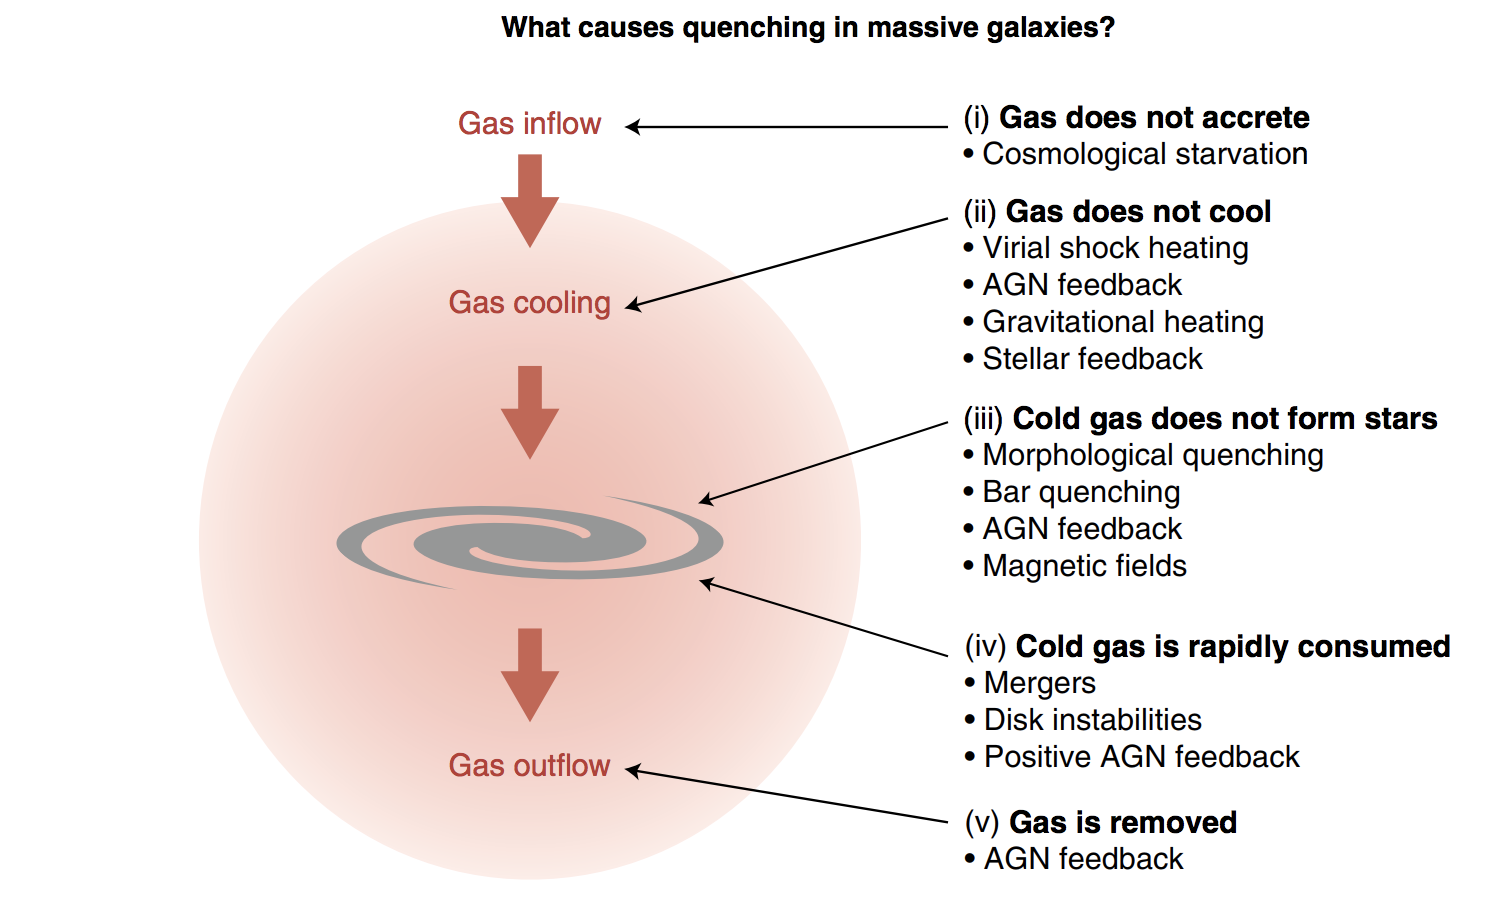
\includegraphics[width=16cm]{figures/quenching.png}
    \caption{\footnotesize{Schematic diagram listing the plausible quenching mechanisms. Image taken from Man \& Belli (2018).}}
    \label{fig:quenching}
\end{figure}

\begin{itemize}
    \item Gas does not accrete. Massive galaxies may quench because of reduced gas accretion onto their dark matter haloes. This condition has been termed cosmological starvation, and it stands as an example of quenching not driven by feedback. Even if accretion is completely shut of, the gas produced by stellar evolution could still fuel subsequent star formation. Therefore, an additional mechanism may be needed to maintain the galaxy quiescent.
    \item Gas does not cool. In the standard picture of galaxy formation, gas collapses in a dark matter halo and heats up because of virial shocks. Simulations show, however, that the shocks are formed only when the halo is more massive than about $10^{12}\,{\rm M_\odot}$. This mass scale is roughly the same as the scale above which galaxies are observed to be prevalently quiescent, suggesting that virial shock heating may account for the onset of star formation quenching. After the shock, however, the hot halo gas should cool and become available for star formation. To prevent further star formation, additional gas heating is necessary. The most accepted explanation is feedback from radiatively inefficient accretion onto SMBHs (radio-mode feedback), which is only effective in massive haloes with hot gas. Implementations of this feedback yielded the first successful mass-function predictions from semi-analytical models. In addition to BH accretion, other gas heating mechanisms have been proposed. For example, a gas clump or a satellite falling into a massive halo releases potential energy. If this energy can be efficiently used to heat the halo gas through ram pressure or dynamical friction, this could constitute a substantial source of gravitational heating. Evolved stellar populations may also contribute to the gas heating through stellar feedback from type Ia supernovae and from stars on the asymptotic giant branch. Regardless of the energy source, it is likely that only massive haloes, in which the gas is roughly at the virial temperature, can be kept hot efficiently. Heating processes are essential to solve a related problem. In galaxy clusters, the cooling time is short enough that the gas should quickly flow to the centre and trigger intense star formation; but central galaxies are typically quiescent. This ``cooling flow'' problem is fundamentally similar to galaxy quenching but takes place on larger scales.
    \item Cold gas does not form stars efficiently. Quenching may be due to a low star formation efficiency, rather than the absence of fuel. To form stars, cold gas must dissipate its kinetic energy (bulk motions and turbulence). Certain non-thermal processes may be capable of injecting considerable amounts of kinetic energy, such that the dissipation timescale is too long for the gas to settle. The stellar bulge could provide large-scale shear to inject turbulence, thereby stabilizing the gas disk from fragmentation. This process is called morphological quenching (or sometimes `gravitational quenching'), typically acts on timescales longer than a billion years and is only effective at low molecular gas fractions, below about 10\%. A similar mechanism can be caused by the stellar bar. This bar quenching may act on even shorter timescales if the stellar bar forms rapidly. Other potential sources of turbulence injection are low-power AGNs and magnetic fields. Such mechanisms may be responsible for maintaining low star formation rates but are unlikely to be the sole explanation for the abrupt termination of star formation in massive galaxies.
    \item Cold gas is rapidly consumed. If star formation consumes cold gas faster than it is replenished, the galaxy will run out of fuel and become quiescent. This can happen if star formation takes place in efficient bursts, potentially triggered by compressive gas motions and effective angular momentum loss. Major mergers of galaxies have first been invoked as a possible trigger, and more recently violent disk instabilities and positive AGN feedback have also been suggested. Clearly, gas consumption alone can quench star formation only temporarily. Additional mechanisms are required to maintain low star formation rates until the present day.
    \item Gas is removed. The accretion onto SMBHs could release sufficient energy and momentum to expel gas from galaxies. This quasar-mode feedback is most efficiently triggered by major mergers owing to high gas inflow rates. Although rare and short-lived, this process can quench star formation by removing the gas supply from massive galaxies.
\end{itemize}

{\noindent}Observational limitations have also motivated a number of phenomenological classifications proposed in the literature. The most common one is the distinction between mass quenching, which affects massive galaxies, and environmental quenching, which only acts on satellite galaxies and is omitted from the present discussion. Some studies instead use the term halo quenching to indicate a mechanism that relates to the halo mass rather than stellar mass. Another common division is that between internal and external quenching, but this division is ambiguously defined. Other studies distinguish between a slow quenching (also called strangulation or starvation), when some leftover cold gas is still available after the quenching event, and a fast quenching, which indicates an abrupt end of the star formation activity.

{\noindent}Semi-analytical models and, more recently, cosmological hydrodynamical simulations are capable of reproducing the basic properties of quiescent galaxies, such as number counts and colours. In all cases, this is made possible by some form of feedback, generally attributed to AGNs, that heats up the gas only in haloes above a mass threshold. Although this broad agreement is certainly encouraging, the fact that substantially different feedback implementations yield relatively similar galaxy populations is worrying, suggesting that they might have limited power in constraining the physical mechanisms in place. AGN feedback could affect galaxy star formation through different physical processes, and observational studies continue to challenge the validity of the crude feedback recipes applied in cosmological simulations. The intricate connection between galaxies and AGN is crucial to understand quenching. Observationally, the level of suppression of star formation seems to correlate not only with stellar mass, but even more strongly with the surface mass density and central velocity dispersion. However, because galaxy properties are interrelated in a complex way, it is not straightforward to establish causal connections given the observed correlations.

{\noindent} These challenging observations are particularly needed at high redshift, soon after the termination of star formation in massive galaxies. A pressing question is to determine whether recently quenched galaxies possess a significant amount of cold gas. If true, this would challenge the common assumption that galaxies stop forming stars because of a lack of gas, and it would require explanations for the suppression of star formation efficiency. Another priority is to measure the properties of the hot gas in quiescent galaxies. If shock heating is prevalent in massive halos as predicted, one should expect to detect its signature in the circumgalactic medium. Spatially resolved observations could further constrain the origin of gas heating and shocks. Lastly, more detailed observations of gas outflows are needed to determine the importance of ejective processes. Outflows are known to be multi-phase, but it remains debated which phase carries the most mass, and whether most of the gas can escape the deep potential well of massive galaxies.

{\noindent}The essential observation that has driven progress on this subject is summarized in Figure \ref{fig:sfquenching}. It shows that the ratio of stellar mass to total mass reaches a maximum at $V_\mathrm{circ}\sim300\,{\rm km\,s^{-1}}$ or at $M_{DM}\sim10^{12}\,{\rm M_\odot}$. This maximum is $\sim1/5$ of the cosmological baryon fraction, so most baryons in the Universe have not yet made stars. Lower-mass halos have smaller stellar fractions (left panel) and smaller baryon fractions (right panel) because (we believe) the baryons have increasingly been ejected from DM halos by star-formation and supernova feedback or never accreted after cosmological reionization. But the focus here is on higher DM masses. They, too, have smaller stellar mass fractions than at the ``sweet spot'' halo mass of $10^{12}\,{\rm M_\odot}$. But Figure \ref{fig:sfquenching} (right) shows that these baryons are not ``missing'' at $M_{DM}\gg10^{12}\,{\rm M_\odot}$. On the contrary, the total baryon fraction converges to essentially the cosmological value in the highest-mass halos, which are halos of rich clusters of galaxies. This is the by-now well known result that, as $M_{DM}$ grows above $10^{12}\,{\rm M_\odot}$ and $V_\mathrm{circ}$ grows above $300\,{\rm km\,s^{-1}}$, an increasingly large fraction of the baryons are indeed present but have not made stars. Rather, they are suspended in hot, X-ray-emitting gas, until in rich clusters of galaxies, that hot gas outmasses the stellar galaxies in the cluster by $1.0\pm0.3\,{\rm dex}$. This has led to the essential idea of ``$M_\mathrm{crit}$ quenching'' of star formation by X-ray-emitting gas, which can happen provided that the DM mass is larger than the critical mass, $M_{DM}\gtrsim M_\mathrm{crit}\simeq10^{12}\,{\rm M_\odot}$, that is required to support the formation and retention of hot gas halos.

\begin{figure}[h]
    \centering
    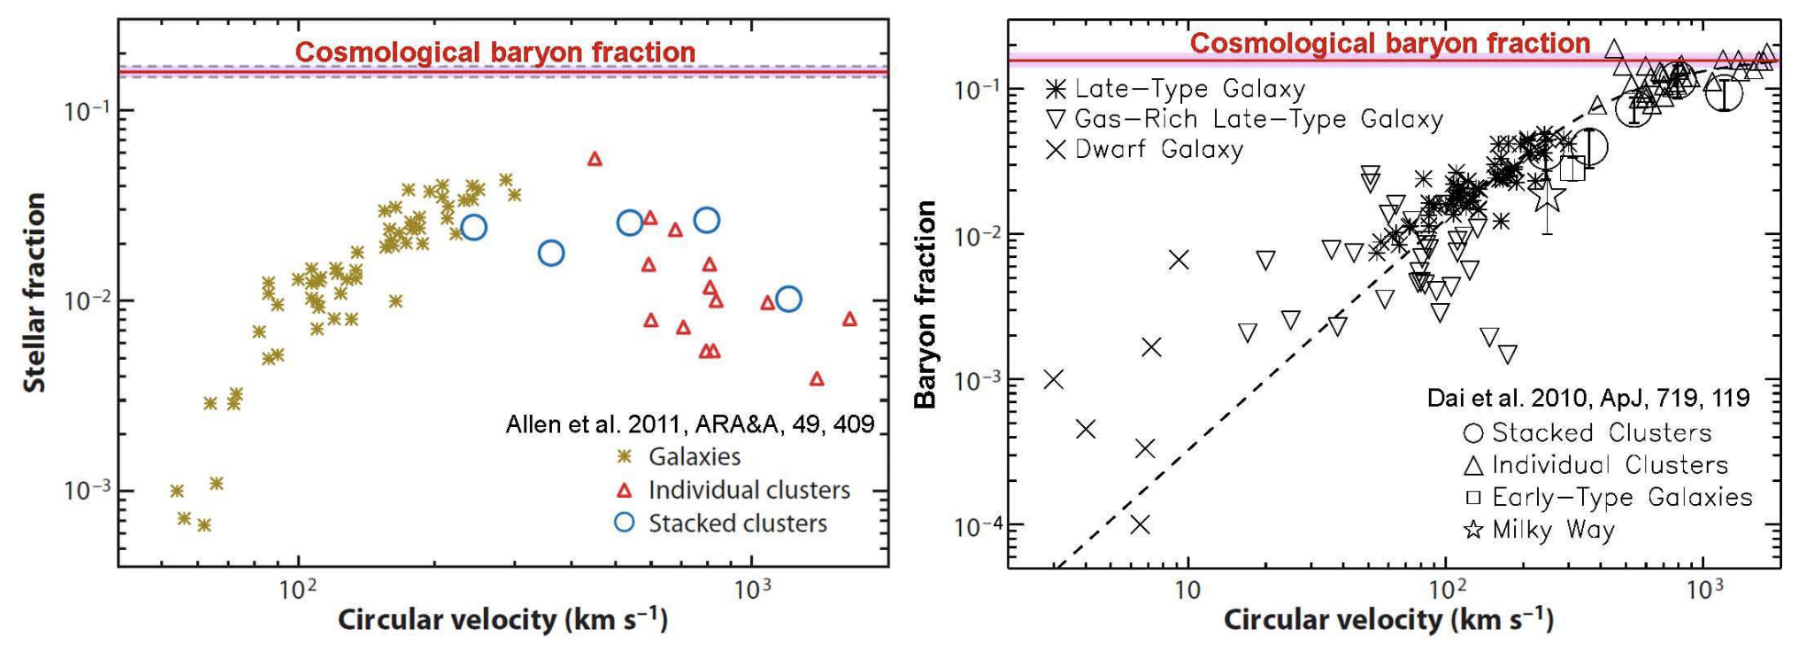
\includegraphics[width=16cm]{figures/SFquenching.png}
    \caption{\footnotesize{Stellar mass fraction $M_∗/(M_\mathrm{baryon}+M_{DM})$ (left) and total baryon mass fraction $M_\mathrm{baryon}/(M_\mathrm{baryon}+M_{DM})$ (right) versus a circular-orbit rotation velocity $V_\mathrm{circ}\sim \sqrt{GM_\mathrm{DM}/r}$ that approximately characterizes the total mass distribution. Here $M_∗$ is the stellar mass, $M_{DM}$ is the DM halo mass, $r$ is the radius of the halo, and $G$ is the gravitational constant. The cosmological baryon fraction has been adjusted very slightly to $0.16\pm0.01$, i.e., the mean of the WMAP and Planck measurements. Both figures originally come from Dai et al. (2010). Image taken from Kormendy (2015).}}
    \label{fig:sfquenching}
\end{figure}

{\noindent}The transition mass between galaxies that should contain X-ray gas and those that should not is consistently derived by a variety of theoretical arguments and is consistency checked via a variety of observational tests. It should occur at the DM mass at which the hot gas cooling time is comparable to the infall time. It has been shown from SPH simulations that gas that is accreted during hierarchical clustering falls gently into shallow potential wells and makes star-forming disks, whereas gas crashes violently onto giant galaxies and is shock-heated to the virial temperature. It is this hot gas that quenches star formation. Calculated hot-gas cooling times are short; this led to the well known ``cooling flow problem'' (Fabian 1994). But X-ray measurements of temperature profiles now show that they are much shallower than cooling-time calculations predict in the absence of heating. Debate continues about how the gas is kept hot; it has been suggested that the required heating is caused by continued accretion; AGN feedback is another candidate, and dying stars returning gas to the IGM at just the right kinetic temperature. The engineering details need to be sorted out. It is likely that all processes are important. The important point is that the galaxies and clusters tell us that they know how to keep the gas hot.

{\noindent}Hydrodynamical simulations of disk formation show that SF in the gas disks is far too efficient, consuming the available gas in too short a time, so that most of the stars would be formed at high redshift, with little current star formation left. Furthermore, the resulting disks are too concentrated and too small, leading to rotation curves which are declining outwards beyond the (small) half-light radius of the disk, in marked contrast with observed rotation curves. This together is known as the overcooling problem in galaxy evolution. Real disk galaxies have a slower conversion of gas into stars and their disks remain larger. And finally, the efficient conversion of gas into stars in our simple model would predict that the stellar mass density in the Universe is much higher than observed -- whereas $\omega_b\sim0.04$, the density parameter in stars is less than 1\%. Hence, most baryons in the Universe have not been converted to stars.

{\noindent}Since stars form out of gas, and the gas distribution is much more extended than the stellar distribution, stars can only form at places in the disk where the gas mass density exceeds a certain value. Marteen Schmidt discovered in 1959 a relation between the surface mass density of gas, $\Sigma_\mathrm{gas}$ (measured in units of ${\rm M_\odot\,pc^{-2}}$) and the star-formation rate per unit area, $\Sigma_\mathrm{SFR}$ (measured in units of ${\rm M_\odot\,year^{-1}\,pc^{-2}}$), of the form

\begin{align*}
    \Sigma_\mathrm{SFR} \propto \Sigma_\mathrm{gas}^\alpha ~ [{\rm M_\odot\,year^{-1}\,pc^{-2}}]
\end{align*}

{\noindent}with a power-law index of $\alpha\approx1.4$. The connection between the two quantities was later examined in detail by Rob Kennicutt, and the relation is known as Schmidt-Kennicutt law; including the normalization, one finds

\begin{align*}
    \frac{\Sigma_\mathrm{SFR}}{{\rm M_\odot\,year^{-1}\,kpc^{-2}}} = (2.5\pm0.7)\times10^{-4} \left(\frac{\Sigma_\mathrm{gas}}{{\rm M_\odot\,pc^{-2}}}\right)^{1.4\pm0.15}.
\end{align*}

\begin{figure}[h]
    \centering
    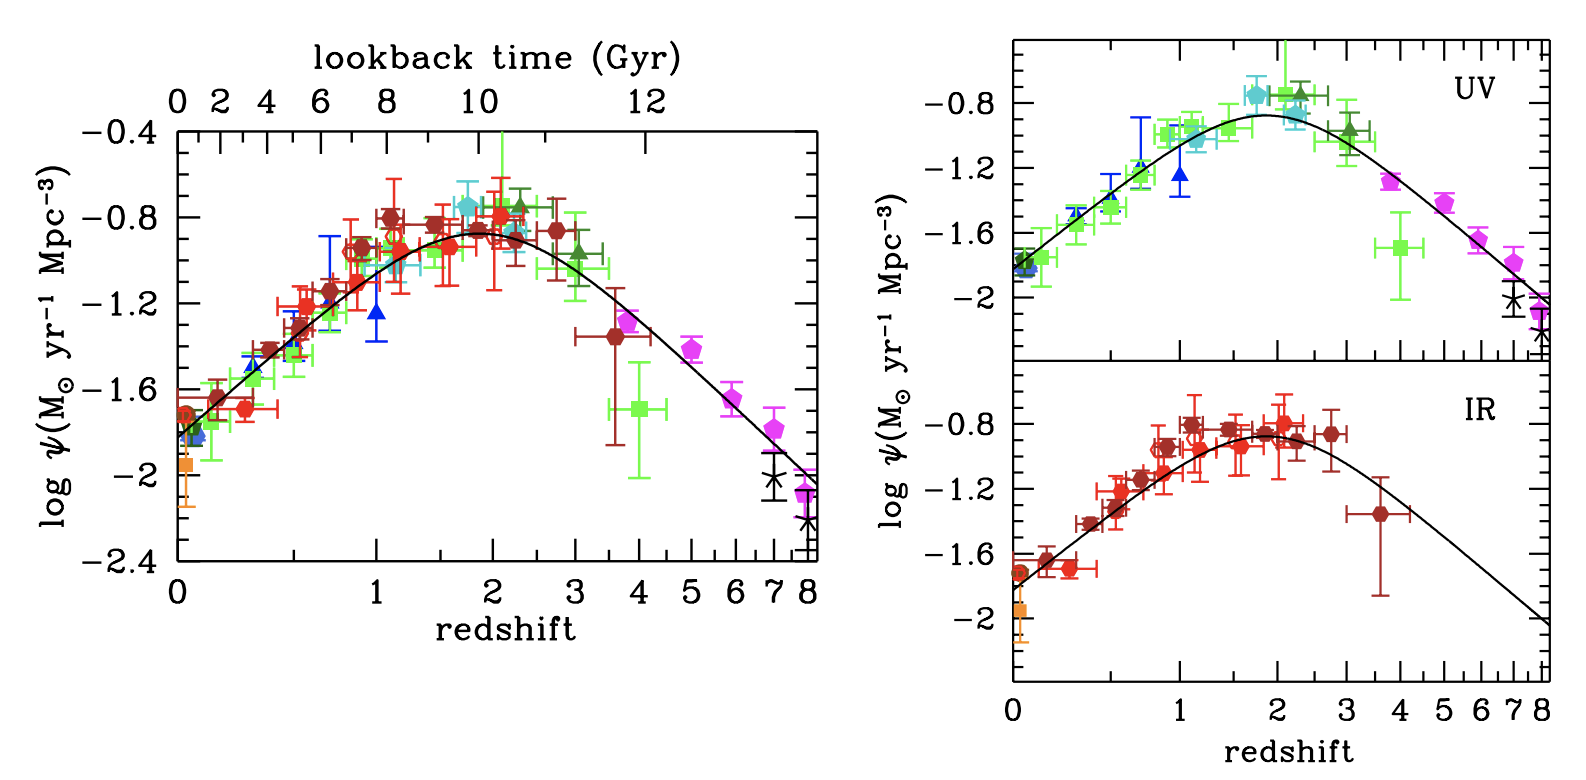
\includegraphics[width=16cm]{figures/SFhistory.png}
    \caption{\footnotesize{The history of cosmic star formation from (top right panel) FUV, (bottom right panel) IR, and (left panel) FUV+IR rest-frame measurements. The solid curve in the three panels plots the best-fit SFRD. Image taken from Madau \& Dickinson (2014).}}
    \label{fig:sfhistory}
\end{figure}

{\noindent}Figure \ref{fig:sfhistory} shows the cosmic SF history from UV and IR as well as the best fitting function

\begin{align*}
    \psi(z) = 0.015\frac{(1+z)^{2.7}}{1+[1+z/2.9]^{5.6}} ~ [{\rm M_\odot\,year^{-1}\,Mpc^{-3}}].
\end{align*}

{\noindent}These state-of-the-art surveys provide a remarkably consistent picture of the cosmic SF history: a rising phase, scaling as $\psi(z)\propto(1+z)^{-2.9}$ at $3\lesssim z\lesssim8$, slowing and peaking at some point probably between $z=2$ and $z=1.5$, when the Universe was $\sim3.5\,{\rm Gyr}$ old, followed by a gradual decline to the present day, roughly as $\psi(z)\propto(1+z)^{2.7}$. The increase in $\psi(z)$ from $z\sim8$ to $z\sim3$ appears to have been steady, with no sharp drop at the highest redshifts, although there is now active debate in the literature about whether that trend continues or breaks at redshifts $9$ and beyond. Although a fitting function was adopted that is a double power-law in $(1+z)$, the SFRD data at $z<1$ can also be fit quite well by an exponential decline with cosmic time and an e-folding timescale of $3.9\,{\rm Gyr}$.

\subsubsection{Follow-up Questions}

\begin{itemize}
    \item What is the SF history of the Universe, and how does it evolve with time? (i.e., Lilly-Madau plot.)
    \item At what redshift was the SF rate the highest?
    \item How does this relate to the population of stars we see today (i.e., how old the Sun is, which stars are most common etc.)?
\end{itemize}

% --------------------------------------------------------------
%               15. 
% --------------------------------------------------------------

\newpage
\subsection{Question 15}

Provide three examples of ways in which feedback processes are important on galactic and intergalactic scales.

\subsubsection{Short answer}

Examples include:

\begin{itemize}
    \item \textbf{Feedback by supernovae}. Very shortly after star formation sets in, the most massive stars of the stellar population undergo a core-collapse supernova which heats the gas and reduces its star formation efficiency.
    \item \textbf{AGN feedback}. In the case of galaxy clusters, the AGN can insert hot bubbles into the ICM through radio jets. Additionally, the strong radiation field from the quasar can change the ionization structure of the surrounding gas which in turn affects its cooling curve and therefore its efficiency of star formation.
    \item \textbf{Ram-pressure stripping and strangulation}. As a galaxy orbits a cluster, it moves relative to the hot ICM which creates a pressure force on the ISM of the galaxy which can remove the gas if it is greater than the gravitational force of the galaxy.
    \item \textbf{Cannibalism}. Galaxies in a cluster can can lose angular momentum and sink to the center where they can merge with other galaxies, becoming `cannibalized' by other cluster members.
\end{itemize}

\subsubsection{Additional context}

{\noindent}\textbf{Feedback by supernovae:} In order to balance the efficient gas cooling, heating sources need to be considered. An unavoidable source of heating is the energy injected into the ISM by supernovae. Very shortly after star formation sets in, the most massive stars of the stellar population undergo a core-collapse supernova. The mechanical energy of the explosion is partly transferred to the gas surrounding the exploding star. Thereby the gas is heated, causing it to expand, thus to decrease its density, which in turn reduces its cooling efficiency. Note that this is a feedback process -- the higher the star formation rate, the more energy is injected into the interstellar gas to prevent, or at least delay, further SF. Depending on the efficiency of this feedback, the local gas of the disk may be blown out of the disk into the halo (and produce a hot gas corona outside the disk), or, in particular for low-mass halos, be removed from the halo through outflowing gas.

{\noindent}In fact, there is direct observational evidence of the occurrence of outflows from star-forming galaxies. For example, the spectra of Lyman-break galaxies reveal substantial mass outflows, at a similar rate as their star-formation rate and with velocities of several hundreds of ${\rm km\,s^{-1}}$.

{\noindent}The details of this feedback process are somewhat uncertain -- how much of the supernova energy is converted into heat, and how much is transferred to the ISM in form of bulk kinetic energy, is not well determined. Furthermore, the feedback by supernovae depends on the assumed initial mass function of stars, which yields the fraction of newly formed stars which explode as core-collapse supernova. The flatter the IMF at the high-mass end, the more supernova energy per unit mass of newly formed stars is injected.

{\noindent}Assuming a universal IMF, the energy released by supernovae per unit mass of newly-formed stars is $\eta_\mathrm{SN}E_\mathrm{SN}$, where $\eta_\mathrm{SN}$ denotes the expected number of supernovae per unit mass of formed stars, and $E_\mathrm{SN}$ is the energy released per supernova. If we assume that this energy reheats some of the cold gas back to virial temperature of the halo, the amount of gas that is reheated after formation of a group of stars with mass $\Delta m_*$ is

\begin{align*}
    \Delta m_\mathrm{reheat} \sim \epsilon\frac{\eta_\mathrm{SN}E_\mathrm{SN}}{V_{200}^2}\Delta m_* ~ [{\rm M_\odot}],
\end{align*}

{\noindent}where $\epsilon$ parametrizes the efficiency of the reheating process. The reheated gas may be transferred back to the hot gaseous halo, whereas other models assume that the reheated gas is first ejected from the halo, and only later reincorporated into the hot halo on the dynamical time-scale of the halo. This ejection scenario effectively delays the time at which the reheated gas can cool and becomes available for star formation again.

{\noindent}As can be seen from the above equation, supernova feedback is more efficient at suppressing star formation in low-mass galaxies -- which is due to the fact that the binding energy per unit mass is an increasing function of halo mass. This simply expresses the fact that for low-mass halos it is easier to drive the gas outwards.

{\noindent}\textbf{AGN feedback:} Whereas supernova feedback explains a decreasing conversion of gas into stars with decreasing halo mass, and thus can account for the difference of the slopes between the galaxy luminosity function and the halo mass function at the low mass/luminosity end, it is less efficient for higher-mass halos, due to the larger $V_{200}$. The increase of the cooling time for higher-mass halos by itself cannot account for the abrupt exponential decrease of the galaxy luminosity function beyond $L^*$. One requires another process which delays the cooling of gas in high-mass halos.

{\noindent}For very massive halos, we have already encountered such a process: the suppression of cooling flows in galaxy clusters is due to AGN activity of the central galaxy in the cluster. Since (almost) all massive galaxies contain a supermassive black hole, this kind of feedback may be operational not only in groups and clusters, but actually in individual massive galaxies as well. In particular, there is a great deal of evidence for a relation between nuclear starbursts in galaxies and AGN activity. The gas needed for a starburst in the center of a galaxy is also potential fuel for the central black hole. Again, the details of this process are quite uncertain, but with plausible prescriptions, the cut-off of the luminosity function at $L\gtrsim L^*$ can be successfully modeled.

{\noindent}Feedback by an AGN can occur in several ways. In the case of galaxy clusters, the major effect of the AGN is the insertion of hot bubbles into the intracluster medium (ICM) through radio jets. The AGNs in most central cluster galaxies are not very luminous, and seem to be in the `radio mode' of low accretion rate. Thus, for low accretion rates, the main channel of feedback is the injection of mechanical energy into the surrounding gas. At high accretion rates, in the `quasar mode', the main source of feedback is presumably heating of the gas. Furthermore, the strong radiation field from quasars changes the ionization structure of the surrounding gas, which affects its cooling curve compared and at low temperatures actually leads to radiative heating. These various effects should be included in realistic models of the evolution of galaxies, at least in an approximate way.

{\noindent}\textbf{Ram-pressure stripping and strangulation:} As a galaxy orbits in a cluster, it moves relative to the hot ICM. In the rest frame of a galaxy, the ICM acts like a wind, with the wind speed equal to the orbital velocity of the galaxy. This wind causes a pressure force on the ISM of the galaxy; it is proportional to the density of the ICM and the square of the velocity. If this force is stronger than the gravitational force of the galaxy which hosts the interstellar gas, this gas can be removed from the galaxy. This ram-pressure stripping can thus over time turn a gas-rich disk galaxy into a disk galaxy without gas (i.e., a spiral galaxy into an S0 galaxy). This effect may be the origin of the larger abundance of S0 galaxies in clusters than in the field population. It also provides a natural explanation for the Butcher-Oemler effect, which states that clusters of galaxies at higher redshift contain a larger fraction of blue galaxies. The blue (spiral) galaxies that have existed at higher redshift may have turned into S0 galaxies in the meantime. The fact that the fraction of ellipticals in a cluster remains rather constant as a function of redshift, whereas the abundance of S0 galaxies increases with decreasing $z$, indicates the importance of the latter process as an explanation of the Butcher-Oemler effect.

{\noindent}Gas which is removed from the galaxies is chemically enriched. The metallicity of the ICM is believed to be due to the mixing of this enriched gas with the ICM. Hence, the metals of the ICM have been generated by earlier stellar populations in cluster galaxies. The efficiency of this effect, as well as that of harassment, depends on the orbit of the galaxy. If the orbit comes close to the inner part of the cluster where the gas and galaxy number density are large, all the gas may be removed, whereas otherwise, only the outer, more loosely bound gas is lost. In this case, the galaxy retains its gas in the inner part and may continue to form stars for a while; only when this gas supply is exhausted, it then turns into a red galaxy, since no new gas can be gained from cooling or accretion. This effect is called strangulation.

{\noindent}\textbf{Cannibalism:} The orbit of a galaxy in a cluster is affected by dynamical friction; it loses energy and angular momentum, and so its orbit will shrink in time. The efficiency of this effect again depends on the galaxy orbit; the closer it comes to the inner parts of the cluster, the stronger are the gravitational friction forces. Furthermore, it depends on the galaxy mass, with more massive galaxies being affected more strongly. Depending on the orbital parameters, a cluster galaxy can lose most of its angular momentum in a Hubble time, sink to the center, and there merge with the central galaxy. By this process, the central galaxy becomes more massive, as it `cannibalized' other cluster members. The aforementioned mass dependence may lead to an increase of the mass and luminosity difference between the brightest cluster galaxy and the second-brightest one.


\newpage
\subsubsection{Follow-up Questions}

\begin{itemize}
    \item What is the star formation rate in the galaxy (derive this)? 
    \item How fast would all the gas be eaten up if there was no feedback?
    \item How could you observationally constrain metal enrichment of the IGM?
    \item How do these processes affect a single galaxy (i.e., not a cluster)?
    \item If feedback sets an effective maximum mass for a galaxy, can you draw a cooling curve (i.e., density versus temperature)? 
\end{itemize}

% --------------------------------------------------------------
%               Resources 
% --------------------------------------------------------------

\newpage
\subsection{Resources}

\begin{itemize}
    \item Extragalactic Astronomy and Cosmology; Schneider (2006)
    \item High Energy Astrophysics; Longair (2011)
    \item An Introduction to Modern Astrophysics; Carroll \& Ostlie (2007)
    \item Gaseous Nebulae and Active Galactic Nuclei; Osterbrock \& Ferland (2005)
    \item Spectral Evolution of Galaxies; Charlot (1996)
    \item Galaxies in the Universe; Sparke \& Gallagher (2005)
    \item Elliptical Galaxies and Bulges of Disk Galaxies: Summary of Progress and Outstanding Issues; Kormendy (2015)
    \item Galactic Dynamics; Binney \& Tremaine (2008)
    \item Star Formation Quenching in Massive Galaxies; Man \& Belli (2018)
    \item Cosmic Star-Formation History; Madau \& Dickinson (2014)
    \item The Type Ia Supernova Width-Luminosity Relation; Pinto \& Eastman (2018)
\end{itemize}


\end{document}
